% !TEX TS-program = xelatex
% !TEX encoding = UTF-8 Unicode
\documentclass[a4paper, 12pt, oneside]{book}

\usepackage{threeparttable}

\usepackage{adjustbox}
\usepackage{longtable}
% \usepackage{subfigure}
\usepackage{subfig}
\usepackage{makecell}
\usepackage{cite}
\usepackage{notoccite}
%\usepackage{chapterbib}
%The chapterbib package facilitates multiple bibliographies in a LATEX document
\usepackage[hyphens]{url}
%Verbatim with URL-sensitive line breaks.
\usepackage[colorlinks=true,linkcolor=black,citecolor=black,filecolor=blue,urlcolor=black,unicode]{hyperref}
%The hyperref package is used to handle cross-referencing commands in LaTeX to produce hypertext links in the document. The package provides backends for the \special set defined for HyperTeX DVI processors; for embedded pdfmark commands for processing by Acrobat Distiller (dvips and Y&Y¡¦s dvipsone); for Y&Y¡¦s dviwindo; for PDF control within pdfTeX and dvipdfm; for TeX4ht; and for VTeX¡¦s pdf and HTML backends.

\usepackage{verbatim}
%The verbatim environment  simply reproduces every character you input, including all  s p a c e s!
\usepackage{color}
%you can set the color of the font of the text, and set the background color of the page.
\usepackage[dvipsnames]{xcolor}
%xecolor package is a simple package which defines about 140 different colors by XeTeX's font
\usepackage{graphicx}
%Standard LaTeX graphics.
% \usepackage{array}
%The array environment is used to make a table of information, with column alignment (left, center, or right) and optional vertical lines separating the columns.
%\usepackage{gensymb}
%Provides generic commands \degree, \celsius, \perthousand, \micro and \ohm which work both in text and maths mode.
\usepackage{indentfirst}
%Make the first line of all sections etc., be indented by the usual paragraph indentation. This should work with all the standard document classes. This minimalist package is part of the "tools" bundle in the LaTeX required distribution.
\usepackage[ruled,linesnumbered]{algorithm2e}
%\usepackage{algorithm}
%\usepackage{algpseudocode}
%A suite of tools for typesetting algorithms in pseudo-code. The algorithmicx package provides many possibilities to customize the layout of algorithms. You can use one of the predefined layouts (pseudocode, pascal and c and others), with or without modifications, or you can define a completely new layout for your specific needs.
\usepackage{enumitem}
%Control layout of itemize, enumerate, description.  It supersedes both enumerate and mdwlist (providing well- structured replacements for all their funtionality), and in addition provides functions to compute the layout of labels, and to 'clone' the standard environments, to create new environments with counters of their own.
\usepackage{mfirstuc}
%\makefirstuc{¡qstuff ¡r} This makes the first object of ¡qstuff ¡r uppercase unless ¡qstuff ¡r starts with a con- trol sequence followed by a non-empty group, in which case the first object in the group is converted to uppercase.
\usepackage{fancyvrb}
%This package provides very sophisticated facilities for reading and writing ver- batim TEX code.
\usepackage{amsfonts}
%TeX fonts from the American Mathematical Society.
\usepackage{ifmtarg}
%If-then-else command for processing potentially empty arguments.
\usepackage{amsmath}
%The amsmath package is a LATEX package that provides miscellaneous enhance- ments for improving the information structure and printed output of documents that contain mathematical formulas.
\usepackage{amssymb}
% Math symbols
\usepackage[mathcal]{euscript}
%This file sets up some font shape definitions to use the Euler script symbols in math mode.
\usepackage[notbib]{tocbibind}
%Add (or disable) bibliography/index/contents to Table of Contents.
\usepackage{rotating}
%Rotation tools, including rotated full-page floats.
%\usepackage{hhline}
%The command \hhline produces a line like \hline, or a double line like \hline\hline, except for its interaction with vertical lines. The command takes a preamble (rather like the preamble of a tabular environment), and this specifies whether there are to be one or two horizontal lines, and what happens when the horizontal line meets a vertical one. The package is part of the tools bundle in the LaTeX required distribution.
\usepackage{wallpaper}
%Easy addition of wallpapers (background images) to LaTeX documents, including tiling.
\usepackage{pdfpages}
%Include PDF documents in LaTeX.
\usepackage{pst-fractal,pst-exa}
% The package will draw the Julia and Mandelbrot sets, the Sierpinski triangle, Koch flake, and Apollonius Circle as well as fractal trees (which need not be balanced) with a variety of different parameters (including varying numbers of iterations).

%Define \XeTeX \XeLaTeX command
\def\reflect#1{{\setbox0=\hbox{#1}\rlap{\kern0.5\wd0
 \special{x:gsave}\special{x:scale -1 1}}\box0 \special{x:grestore}}}
\def\XeLaTeX{\leavevmode
 \setbox0=\hbox{X\lower.5ex\hbox{\kern-.15em\reflect{E}}\kern-.08em\LaTeX}%
 \dp0=0pt\ht0=0pt\box0}
 \def\XeTeX{\leavevmode
 \setbox0=\hbox{X\lower.5ex\hbox{\kern-.15em\reflect{E}}\kern-.08em\TeX}%
 \dp0=0pt\ht0=0pt\box0}

% \usepackage[none]{hyphenat}  %hyphenation package

% Start Declare physics symbols
\newcommand{\gv}[1]{\ensuremath{\mbox{\boldmath$ #1 $}}} 
\newcommand{\grad}[1]{\gv{\nabla} #1} % for gradient
\let\divsymb=\div % rename builtin command \div to \divsymb
\renewcommand{\div}[1]{\gv{\nabla} \cdot #1} % for divergence
\newcommand{\curl}[1]{\gv{\nabla} \times #1} % for curl
\let\baraccent=\= % rename builtin command \= to \baraccent
\renewcommand{\=}[1]{\stackrel{#1}{=}} % for putting numbers above =
%end Declare

\usepackage{booktabs}				% ªí®æ½u±ø
\usepackage{tabularx}
%tabularx, is defined, which takes the same arguments as tabular*, but modifies the widths of certain columns, rather than the inter column space, to set a table with the requested total width. The columns that may stretch are marked with the new token X in the preamble argument. This package requires the array package. The package is part of the tools bundle in the LaTeX required distribution.
%\usepackage{lmodern}
%The Latin Modern family of fonts consists of 72 text fonts and 20 mathematics fonts, and is based on the Computer Modern fonts released into public domain by AMS (copyright c 1997 AMS).
%\font\lmr="[lmroman10-regular]"

\usepackage{fix-cm}
% fix-cm which will allow you to use the fonts, within LaTeX, at any size you choose.

%\usepackage{listings}
%Typeset source code listings using LaTeX.
%\usepackage{textcomp}
%provide many text symbols (such as baht, bullet, copyright, musicalnote, onequarter, section, and yen)

\usepackage{amsthm}
%The package facilitates the kind of theorem setup typically needed in American Mathematical Society publications. The package offers the theorem setup of the AMS document classes (amsart, amsbook, etc.) encapsulated in LaTeX package form so that it can be used with other document classes. Amsthm is part of the (required) AMS-LaTeX distribution, so should be present in any LaTeX distribution.
\newtheorem{mydef-no-caption}{Definition}
\newenvironment{mydef}[1][]%
	{\begin{mydef-no-caption}{\ifnotmtarg{#1}{\textnormal{(\textbf{#1})}~}}}%
	{\end{mydef-no-caption}}

\usepackage{numprint}
%Print numbers with separators and exponent if necessary.
\npthousandsep{,}
\npthousandthpartsep{}
\npdecimalsign{.}

\usepackage{multirow}
%Create tabular cells spanning multiple rows.

\usepackage{ntu}
%NTU thesis style file
\hypersetup{
	pdfauthor={\theauthorEN{}},
	pdftitle={\thetitleEN{}},
	pdfsubject={NTU Thesis}
}

\usepackage{setspace}
%Set space between lines.

\usepackage[absolute]{textpos}
%Place boxes at arbitrary positions on the LaTeX page.
\lstdefinestyle{nonumbers}{numbers=none}
\textblockorigin{0mm}{0mm}

\setcounter{tocdepth}{2}

\pagestyle{plain}

\usepackage{url}
\usepackage{colortbl}
\usepackage{CJKnumb}
\usepackage{titletoc}					% 目錄修改套件
\usepackage{titlesec} 				% 美化章節標題套件

% === 圖表相關設定 ===

\graphicspath{{images/}} 			% 設定圖形路徑

\newcommand{\loflabel}{圖}
\newcommand{\lotlabel}{表}
\renewcommand\figurename{\loflabel}
\renewcommand\tablename{\lotlabel}
\setlength{\abovecaptionskip}{10pt} % 修改圖表標題和圖表內容的間距
\setlength{\belowcaptionskip}{10pt} % 修改圖表標題和圖表內容的間距

% === 自訂指令 ===
\renewcommand\contentsname{目次}
\renewcommand\listfigurename{圖次}
\renewcommand\listtablename{表次}
\renewcommand\bibname{參考文獻}

\setlength{\parindent}{22pt}  	% 設定縮排
% \setlength{\lineskip}{1.5em}	% 設定行間距
% \setlength{\parskip}{0.5em}	% 設定段落間距

\newboolean{isAppendix}
\setboolean{isAppendix}{false}


% === 目錄標題 (配合 titletoc) ===
\titlecontents{chapter}[0em]{\fontsize{12}{18}\selectfont}
  {\hspace{3.5em}\contentslabel[第\CJKnumber{\thecontentslabel}章]{3.5em}}
  {}{\hspace{0.5em}\titlerule*{.}\contentspage}

\titlecontents{section}
[3.5em]
{\fontsize{12}{18}\selectfont}
{\contentslabel{2em}}
{}{\hspace{0.5em}\titlerule*{.} \contentspage}

\titlecontents{subsection}
[6.5em]
{\fontsize{12}{18}\selectfont}
{\contentslabel{3em}}
{}{\hspace{0.5em}\titlerule*{.} \contentspage}

% === 章節標題 (配合 titlesec) ===
\titleformat{\chapter}[display]
	{\bf\Large}
	{\filleft 第\,\CJKnumber{\thechapter}\,章}
	{1ex}
	{\huge\titlerule
	 \vspace{2ex}%
	 \filright}
	[\vspace{2ex}%
	 \titlerule]
\begin{document}

%----------- hyphenation  -----------
%\righthyphenmin=10  % Best hyphenation parameter

%----------- watermark -----------
\CenterWallPaper{0.174}{figure/watermark.jpg}
\setlength{\wpXoffset}{6.1725cm}
\setlength{\wpYoffset}{10.5225cm}

%----------- cover page -----------
\maketitle

%----------- side page, used for printing on spline -----------
% \makeside

\frontmatter
%----------- generate the certification page by LaTeX -----------
% \makecertification

%----------- include pdf by using package pdfpages -----------
\addcontentsline{toc}{chapter}{口試委員會審定書}

\includepdf[pages={1}]{chenpc.pdf}

\onehalfspacing % 1.5 倍行距
\begin{acknowledgementsCH}
    \fontsize{12pt}{18pt}\selectfont
    整本論文僅剩誌謝需要撰寫是多麼奢侈的一件事。首先感謝百忙抽空來擔任考試委員的徐瑋勵老師與張秉純老師,
    針對研究與論文提出寶貴建議,使本論文更加完整。謝謝在碩士班期間指導我的詹魁元老師,
    老師總是希望我們能主動去尋找自己的研究方向,雖然有時會有些天馬行空的想法,
    從碩一的機械手臂、步態分析、IMU 動作量測、訊號處理,研究主題跟計劃助理的更換頻率一樣高,直到碩二才逐漸穩定,
    但正是在這飄搖不定的研究主題中探索,也才能真正體會到研究的五味雜陳,除了感謝老師的指導外,也謝謝老師適時的給予信心,
    還有能加入 SOLab 的機會,很開心也很榮幸地順利完成了碩士學位。

    長幼有序,首先感謝實驗室的大家長彥智學長,謝謝彥智在研究上的各種協助,像是回答一些在最佳化上的蠢問題,
    感謝一同共患難兩年的柏賢,不管是在運動領域上的常識補充,還是這兩年來的生活瑣碎,都給予了很大的協助,
    敬祝兩位博班學長在未來研究上一帆風順。謝謝詔東在修課與程式上的指導、昱凡在研究上的莫大大大幫助 (尤其是畢業後的學術騷擾)、
    冠成的好奇心使我在研究上的啟發,還有亭宜在研究上的鼓勵,撇除學術上的感謝外,從喝酒、打牌、開趴、出遊,再到電影、火鍋馬拉松,
    學長姊們帶來更多的是生活上的樂趣與動力來源。謝謝同屆一起奮鬥的夥伴們,啟瑞在日常中的閒聊與協助、
    怡萱在千奇百怪問題上的解惑、若瑄在修課期間的各種組隊、重叡都不講話 (但後期真.共患難了數次),以及冠賢在程式上的協助與日常討論,    
    雖每個人的研究領域都隔了一座山,或許不能相互給予實質幫助,但在心靈上絕對是大拇指的,同時也讓我見識到了何謂強者。
    最後也謝謝琮祐、鐘毅、敬亭、問蕖、珮甄、怡葶,協助處理實驗室大小事,祝順利畢業。

    感謝在碩士兩年相互扶持的朋友們,像是同為從成大上來臺大的啟玄、志霖、敬桓和立渝,歡樂的吃飯時光、
    羽球團和爬山都給予生活滿滿動力,雖然說了兩年的基隆行還沒成,另外也還有永和酒友會的名宇和冠丞。
    謝謝高中好麻吉兼吃飯好友振原,在剛來臺大時的協助與後期的職涯關心,謝謝嘉宏、餘之、晴立,
    以及其他仍保持聯繫的朋友們,分享日常瑣碎與相互關心都是菸酒生的生活調劑。此外研究生加入滑板社看似荒謬,
    但卻是我在研究最苦悶時的精神糧食,在此特別感謝佐庭、銘志和品竹。最要感謝的是我的家人,除了實質上的經濟援助外,
    還有心靈上的鼓舞,不僅僅是碩士兩年,而是從出生那刻到現在,沒有您們的栽培,我就不會有現在如此的成就。

    最後,感謝我自己願意相信自己、堅持到底,小時候對臺大的印象是遙不可及的,如今卻在此順利地完成了求學里程,
    期許自己在未來能找到屬於自己合適的位置並發光發熱,不管是在職場、社會,還是自己的人生當中。

    \begin{flushright}
        林易玄 謹誌於\\
        國立臺灣大學 機械工程學系\\
        中華民國一百一十二年七月
    \end{flushright}
 
\end{acknowledgementsCH}
\chapter{中文摘要}
\fontsize{12pt}{18pt}\selectfont

人體姿態量測、估計與重建技術經過多年的發展,已成為一個重要的研究領域。人體姿態量測與重建技術可將人體姿勢量化為關節角度、肢段長度、朝向及關節位置等數據,並應用於醫療診斷與復健、運動訓練指導,以及動畫及遊戲動作模擬等領域,有助於提升醫療水平、運動表現和娛樂體驗。

% 光標記動作捕捉系統因其量測精準的特性,廣受學者們喜愛,但其高昂的成本、複雜的設備架設及對環境光的要求,限制了其應用範圍。近年來,隨著機器學習技術的快速發展,無需光標記及特定實驗服裝的影像辨識技術逐漸成為人體姿態量測的新趨勢,大幅簡化實驗準備工作,但容易受到物體遮擋的影響。為了解決這個問題,許多學者提出了使用 IMU 資訊融合的改進方法,以提高人體姿態重建的成功率。然而,現有的方法多未公開程式碼,或在重建過程中仍需參考光標記動作捕捉系統的資訊,限制了其應用範圍。
光標記動作捕捉系統因其量測精準的特性,廣受學者們喜愛,但其高昂的成本、複雜的設備架設及對環境光的要求,限制其應用範圍。近年來,隨著機器學習技術的快速發展,無需光標記及特定實驗服裝的影像辨識技術逐漸成為人體姿態量測的新趨勢,大幅簡化實驗準備工作,但容易受到物體遮擋的影響。為解決這個問題,許多學者提出使用 IMU 資訊融合的改進方法,以提高人體姿態重建的成功率。然而,現有的方法仍需參考光標記動作捕捉系統的資訊,限制其應用範圍。

% 本研究基於一個開源的融合方法進行改進,建立一系列流程,包含相機校正、建立個人化三維人體模型、時間同步及空間校正,讓每位受試者皆可自行輸入量測資料,進行人體姿態重建,不再侷限於學者們發表的資料集。本研究證實融合 IMU 資訊可以有效提高人體姿態重建的成功率,並達成不需光標記動作捕捉系統輔助,在任何環境下皆可進行人體姿態量測及重建的目標。此外,本研究進一步探討在不影響準確度的前提下,減少使用相機數量進行數據蒐集的可能性,以提高設備的機動性及降低器材架設的複雜度。
本研究基於一個開源的融合方法進行改進,建立一系列流程,包含相機校正、建立個人化三維人體模型、時間同步及空間校正,讓每位受試者皆可自行輸入量測資料,進行人體姿態重建。本研究證實融合 IMU 資訊可以有效使人體姿態重建的成功率提升約 23.8\%,且對於誤差約有 5 \textasciitilde\ 10 (mm) 的改善,並達成不需光標記動作捕捉系統輔助,可在任何環境下進行人體姿態量測及重建的目標。此外,本研究進一步探討在不影響準確度的前提下,減少使用相機數量進行數據蒐集的可能性,以提高設備的機動性及降低器材架設的複雜度。

\bigskip
\textbf{關鍵字:} 人體姿態量測、人體姿態重建、影像辨識、IMU、感測器融合

% \end{abstractCH}

\doublespacing  % 2 倍行距
\begin{abstractEN}

The advancement of technology has significantly broadened the possibilities of research in fields 
such as biomechanics and physiological signals, surpassing the limitations of clinical experiments. 
Through computer simulation and analysis, researchers can also obtain complex results like neural 
signals, muscle force, and joint torque. 
This progress has had unprecedented implications in various domains, including clinical medicine, 
rehabilitation, and sports science. 
However, achieving accurate results in human motion simulation and analysis relies not only on 
the evaluation methods but also on the choice of models. 
While generic models simplify the model-building process, they fail to fully capture the unique 
characteristics of individual subjects. 
Thus, the development of subject-specific models is crucial, albeit challenging.

In this study, the combination of biomechanics software, OpenSim, and mathematical 
computing software, MATLAB, is used to estimate musculotendon parameters in musculoskeletal models 
through optimization methods.
The primary focus of the research centers around prediction tasks. 
Prior to parameter estimation, sensitivity analysis is performed to determine the desired tasks to 
be executed. 
Subsequently, multiple prediction tasks are executed to quantify the discrepancy between the 
predicted trajectories and the target trajectories, enabling the determination of parameter 
values for the evaluated muscles.
Finally, the optimal models resulting from the evaluation process are subjected to model validation 
to ensure their accuracy.
The methodology is demonstrated through several simulation cases using a widely used upper extremity 
musculoskeletal model, confirming the feasibility and effectiveness of the proposed methods.
Moreover, the study investigates the issue of parameter non-identifiability and affirms that 
engaging in multiple prediction tasks is an effective means to circumvent its influence.
In conclusion, the proposed methodology effectively estimates musculotendon parameters in 
musculoskeletal models, providing substantial support for future development of subject-specific models.

\textbf{Key words:} subject-specific musculoskeletal model, Hill-type muscle model, musculotendon parameter estimation, parameter non-identifiability, optimization
\end{abstractEN}

\onehalfspacing
\tableofcontents
\listoffigures
\listoftables
% \input{chapter/SymbolList} % 符號列表

% changes the behavior back to the expected version, and resets the page number
\mainmatter 

\onehalfspacing
%----------- Include/Input your thesis here -----------
% normal cite == \input
% chapter cite  == \include

\chapter{緒論}
\fontsize{12pt}{18pt}\selectfont

% ------------------------- 1.1 ------------------------- %
\section{前言}
% 人體動作模擬發展;應用

% 人體動作模擬種類

% 模型選擇;通用模型;個人化模型

% ------------------------- 1.2 ------------------------- %
\section{研究動機與目的}
% 困境、動機、目的
通過人體姿態的量測與估計及重建,可以將人體的姿勢與動作數據化,從而改善運動員的姿勢、協助影視動畫及遊戲人物的動作模擬、幫助醫學研究及醫療施行~\cite{tsakanikas2020evaluating}~\cite{zhao2017imu},目前最常被用於量測人體姿態及重建的系統為光標記動作捕捉系統,例如 OptiTrack、Vicon 等系統,其量測精準,動作重建方便,成為許多影視公司及動作分析實驗室的必備設備,但因為光標記系統的量測方法以紅外光為通訊媒介,因此量測環境需要嚴格控管環境光,且架設一個實驗場地需耗費許多時間,設備的成本也相對高昂,因此提高了人體姿態量測的使用門檻。

由於光標記動作捕捉系統的門檻限制及現今機器學習快速發展,使用影像辨識重建人體動作的方法越來越受到重視,藉由電腦視覺及機器學習辨別出影像中人體關節點的位置,從而進行人體姿態估計及重建,其事前準備工作簡單,受試者無需黏貼標記點,但是影像辨識容易受到自體或是周圍障礙物的遮擋,導致無法辨識出受遮蔽的關節點。為了解決這個問題,許多學者提出了改進方法,有些學者提出基於機器學習的方法,有些學者則提出使用 IMU 資訊融合,藉由 IMU 較不受遮擋的特性,改善影像辨識在遮擋情況下無法重建的問題。目前雖有許多學者提出有效且準確的融合方法,例如 3DPW~\cite{vonMarcard2018},但這些方法大多未公開程式碼,或是有些方法在重建人體姿態的過程中有參考 Vicon 資訊。因此,在時間有限的情況下,本研究將基於一個程式開源的融合方法進行改進,旨在證實融合 IMU 資訊可以有效提高人體姿態重建的成功率,並達成不需 Vicon 輔助,在任何環境下皆可進行人體姿態量測及重建的目標。

本研究所使用的融合方法,在三維人體模型的建立及定位人體在空間中的位置時,皆參考了Vicon的資訊,且使用的影像辨識模型因為訓練資料庫較單一,對於受試者、服裝、環境的容忍度較低,難以廣泛應用。因此,本研究嘗試更改三維人體模型的建立方法及影像辨識模型,希望在不需Vicon資訊,也不需重新訓練影像辨識模型的情況下,可直接輸入量測資料,重建人體姿態,以期增加影像辨識及IMU融合方法的應用性。此外,本研究進一步探討在不影響準確度的前提下,減少使用相機數量進行數據蒐集的可能性,以期提高設備的機動性及降低器材架設的複雜度。

% 寫目前的研究成果和結論,就是誤差只增加0.5 cm,但是重建的成功率提高8~10%左右→本研究

% ------------------------- 1.3 ------------------------- %
\section{論文架構}
本論文共含有五個章節,其架構如下:

\begin{itemize}
    \item \textbf{第一章:緒論}
    \\ 介紹本論文之研究背景,由研究背景的需求與困境當中,衍生出本研究之動機與目的,闡述本論文之核心目標。
    \item \textbf{第二章:文獻回顧}
    \\ 針對該領域現存的研究進行介紹與整理,包括動作捕捉系統、人體模型種類、時間對齊方法、感測器融合演算法等文獻,進行回顧與討論。
    \item \textbf{第三章:研究方法}
    \\ 介紹本研究所改善之人體姿態估計方法,包含實驗系統設定、相機校正、三維人體模型建立、時間空間對齊等方法,
    除此之外也進一步探討減少相機數量對進行人體姿態估計的影響。
    \item \textbf{第四章:系統驗證之實驗結果與討論}
    \\ 針對第三章所使用之方法,探討減少用於人體姿態估計的相機數量的可能性,評估三維人體模型建立的準確性及討論使用 IMU 進行感測器融和重建人體姿態的必要性。
    \item \textbf{第五章:結論與未來工作}
    \\ 總結本研究之成果與貢獻,並給予適當的建議,作為未來本研究之延伸方向。
\end{itemize}

\clearpage
\chapter{文獻回顧}
\fontsize{12pt}{18pt}\selectfont %字體大小,行距

% ------------------------- 2.0 ------------------------- %
本論文研究主題為評估個人化模型之肌肉參數,在文獻回顧中,首先會介紹關於人體動作量測的技術,
包含動作捕捉系統、感測裝置等介紹,接續會討論關於動作模擬與分析的部分,主要切割為三部分,
前半部將先引入人體模擬流程與系統介紹,並依照複雜程度進行模型分類,後半部則是關於人體的模擬與分析資訊,
最後則會回顧個人化模型的相關文獻,統整現今學者在肌肉參數領域的研究,其針對不同方法來進行介紹,
例如以直接量測或是間接估測來取得肌肉參數。第二章節將圍繞在該研究主題的背景與現況來進行探討,最終闡述肌肉參數的重要性。

% ------------------------- 2.1 ------------------------- %
\section{動作捕捉系統}
% 概述人體動作捕捉,再說分為單感測器動作捕捉系統及多感測器動作捕捉系統,單感測動作捕捉系統又分為光學動作系統及無學動作捕捉系統
% 下面的子段落要寫的:原理、特色、目前可達到的誤差、優缺點
動作捕捉系統為現今常用於擷取人體動作、表情、手勢或其他物體動作等資訊的技術,其可應用於運動分析~\cite{armitano2022swot}、
醫學研究~\cite{alarcon2020upper}~\cite{gu2023imu}、遊戲開發、影片製作等領域,
藉由取得的資訊,可進行分析、模擬、辨識等應用。
根據感測器種類及數量的不同,動作捕捉系統可分為單感測器動作捕捉系統及多感測器融合動作捕捉系統,
其中單感測器動作捕捉系統又可分為光學動作捕捉系統及慣性動作捕捉系統。 

而人體姿態 (pose) 則可使用位置資訊 (position) 或朝向資訊 (orientation) 進行定義,
位置資訊通常以笛卡爾坐標系描述物體在空間中的位置,因此可使用量測結果為位置資訊的光學動作捕捉系統進行姿態追蹤;
而朝向資訊則常以尤拉角 (Euler angles) 、旋轉矩陣 (rotation matrix) 或四元數 (quaternions) 來描述物體的朝向狀態,
因此可使用量測結果為朝向資訊的慣性動作捕捉系統進行姿態追蹤。
以下將針對光學動作捕捉系統、慣性動作捕捉系統、多感測器融合動作捕捉系統,這三大類系統進行介紹。

\subsection{單感測器-光學動作捕捉系統}
% 有沒有光標記的都放在這一段裡面一起描述,可能用句號分開就好
光學動作捕捉系統是目前最常見的動作捕捉系統,其原理為透過辨別標記點或特定特徵點的位置來追蹤物體的運動,再進一步由邊際點或特徵點的位置推估物體的姿態。
根據受試者身上有無光標記 (marker),可將光學動作捕捉系統以有無光標記的分類方法細分為光標記捕捉系統及無標記捕捉系統。

\subsubsection{光標記動作捕捉系統}
% - 量測精確度高,作為目前開發其他動作捕捉系統的標準
% - 無法在室外量測
% - 器材架設不易,價格昂貴
% - 量測誤差約落在 1 公分
光標記 (marker-based) 動作捕捉系統,
如 Vicon ~\cite{vicon_web}是目前最常見且最精準的動作捕捉系統,
其在靜態實驗中,平均絕對定位誤差為 0.15 (mm)~\cite{merriaux2017study},
因此常被當作黃金標準,用於確認其他動作捕捉系統的準確性。
光標記動作捕捉系統所需量測設備為多個紅外光攝影機及多個反光標記點,
反光標記點需黏貼在受試者多處明顯不易被遮擋的部位,例如骨突點,確保在實驗過程中的多數時間可於影像中看見並被記錄,
而已經過校正的多個紅外光攝影機需同時記錄下影像,確保不同角度間的影像無時間差,
每台紅外光攝影機可發出紅外光,也可接收反光標記點反射的紅外光,透過三角測量計算標記點的位置來推估受試者的姿態,
實驗環境及實驗設置如圖~\ref{ch2_fig_OMC_Vicon} 所示。
由於光標記動作捕捉系統主要傳遞訊息的媒介為紅外光,需要嚴格控管環境光(例如陽光)的影響,減少環境光造成的雜訊,
因此實驗環境多為使用人造光為主要照明的的室內,無法在會受到大量陽光干擾的室外進行量測,
且由於需使用多台攝影機,因此器材架設不易,價格昂貴。

\begin{figure}[!ht]
    \centering
    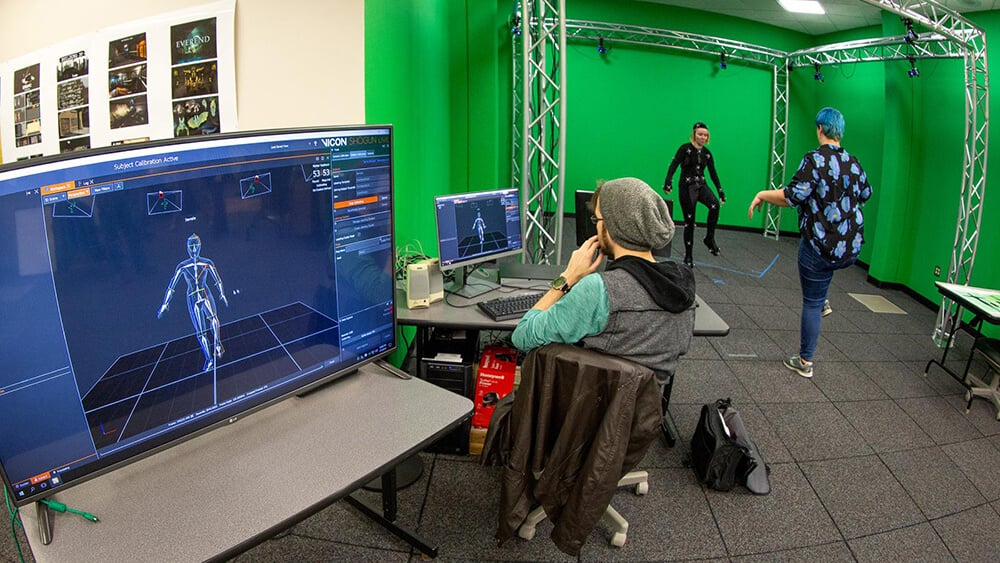
\includegraphics[width=8cm]{figure/ch2_fig_OMC_Vicon.jpg}
     \caption[Vicon 實驗環境與設置]{Vicon 實驗環境與設置}
     \label{ch2_fig_OMC_Vicon}
\end{figure}

\subsubsection{無標記動作捕捉系統}
% - OpenPose、MediaPipe
    % - 看一下 OpenPose 的文獻
    % - 可在室外量測
    % - 器材架設相對容易
    % - 量測誤差約落在 7.2 公分,精準程度會隨著相機數量的減少而降低
    % - 若被遮擋,則無法辨識出被遮擋的關節
    % - 上到下或下到上的辨識(不知道找不找得到相關有提到這方面的paper)
    % - 想想看要怎麼把兩種方法的辨識結果圖片塞進去
因為光標記動作捕捉系統的限制,加上電腦視覺與深度學習的崛起,無標記 (marker-less) 動作捕捉系統逐漸受到重視~\cite{sarafianos20163d},
其中 OpenPose ~\cite{8765346}~\cite{wei2016cpm}~\cite{simon2017hand}~\cite{cao2017realtime}、
由 Google 團隊開發的 MediaPipe ~\cite{mediapipe_web} 及由 Microsoft 開發的 Kinect ~\cite{zhang2012microsoft} 等系統是目前常見的無標記動作捕捉系統,
下方圖~\ref{ch2_fig_rec_result} 為光標記捕捉系統的實際應用。 

透過已經過校正的單一或多個攝影機同時拍攝受試者的影像,利用電腦視覺及深度學習技術辨識出受試者在二維平面上的關節點位置,
辨識關節點位置的方法分為上到下方法 (top-down method) 及下到上方法 (bottom-up method) 兩種~\cite{nie2019single},
上到下方法如圖~\ref{ch2_fig_topvsbottom} 上半部分,
先辨識出受試者的周圍方塊 (detected bounding boxes),再由周圍方塊內的範圍辨識出關節點位置,例如 MediaPipe 即為上到下方法,
其缺點為若在辨識過程中找不到人,無法匡出周圍方塊,則無法辨識出關節點位置,
且計算量會隨著出現在畫面中的人數增加而增加,計算時間也會隨之上升;
下到上方法如圖~\ref{ch2_fig_topvsbottom} 下半部分,
為先偵測到關節,再將關節組成群組,最後形成特定姿勢的方法,例如 OpenPose 即為下到上方法,
計算時間不會因為出現在畫面中的人數增加而增加,計算量也相對較小,
缺點為若受試者沒有完整的出現在畫面中,則有可能辨識點無法組成一個人的群組進而被判斷為一個人,
且也有可能會把非人類,但形狀與人類相似的關節點誤認。

經過影像辨識的圖像的輸出資料為熱圖 (heatmap),將其可視化後如圖~\ref{ch2_fig_heatmap} 所示,
由左至右分別為左肩膀、左手肘、左手腕、右肩膀的熱圖,
有學者會進一步對熱圖進行後處理,例如 OpenPose 將熱圖與其定義的 Part Affinity Fields (PAF) 結合,進一步更準確的辨識出關節點位置,
又或者如 MultiPoseNet 將熱圖與 Pose Residual Network (PRN) 結合,
從熱圖結果中篩選出研究者有興趣的關節點位置~\cite{kocabas2018multiposenet}。
因此,要使用哪一種辨識方法,是否對輸出的熱圖進行後處理,需經過學者們仔細思索自身需求,再進行選擇。
無論選擇哪一種辨識方法,最容易被大眾應用的相機為 RGB 相機 (Red-Green-Blue camera),因此蒐集到的影像資訊缺乏受試者的深度資訊,
需再透過棋盤格方法~\cite{zhang1999flexible} 進行相機校正及三角測量計算,取得受試者的三維姿態。

使用無標記動作捕捉系統進行人體姿態重建時,誤差會受到多個因素影響,
例如輸入影像辨識模型訓練集的多樣性、受試者的姿態及服裝顏色、背景複雜程度、相機校正的準確度、相機的數量等,
因此誤差範圍較廣,例如 OpenPse 使用五台相機進行量測,其誤差約為 30 (mm)~\cite{nakano2020evaluation},
Adafuse 使用八台相機進行測量,其誤差約為 19.2 (mm)~\cite{zhang2020adafuse}。
儘管無標記動作捕捉系統的誤差無法與光標記動作捕捉系統匹敵,
但是,無標記動作捕捉系統較不受環境光限制,因此可以解決實驗場地必須設置於室內的限制,可拓展至室外進行量測,也增加了可量測的範圍及動作多樣性,
且器材架設相對容易,使用手機也可進行影像錄製,架設成本相對較低,
但其缺點為易受到遮擋而影響辨識結果,若受試者的部分關節被自身遮擋或是被場域中的其他障礙物遮擋,則無法辨識出被遮擋的關節。

\begin{figure}[!ht]
    \centering
    \begin{minipage}{.5\textwidth}
      \centering
      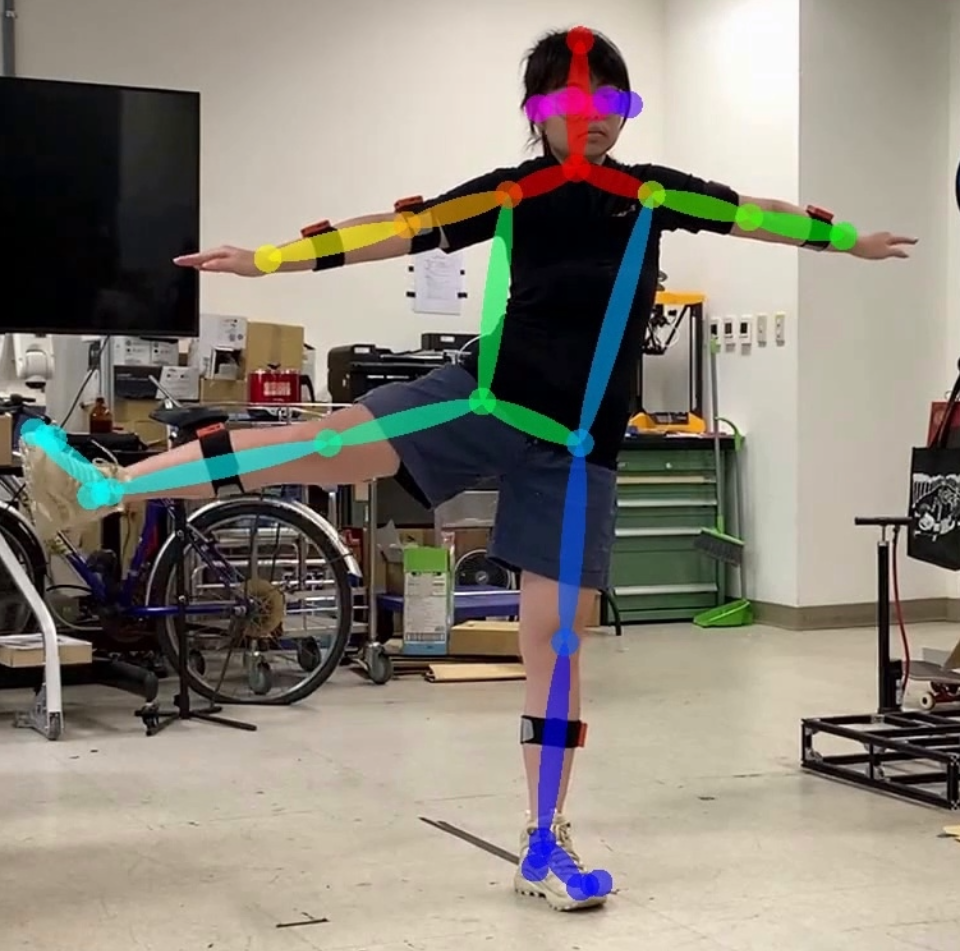
\includegraphics[width=\linewidth]{figure/ch2_fig_rec_openpose.png}
      \caption*{(a) OpenPose}
    \end{minipage}%
    \begin{minipage}{.5\textwidth}
       \centering
       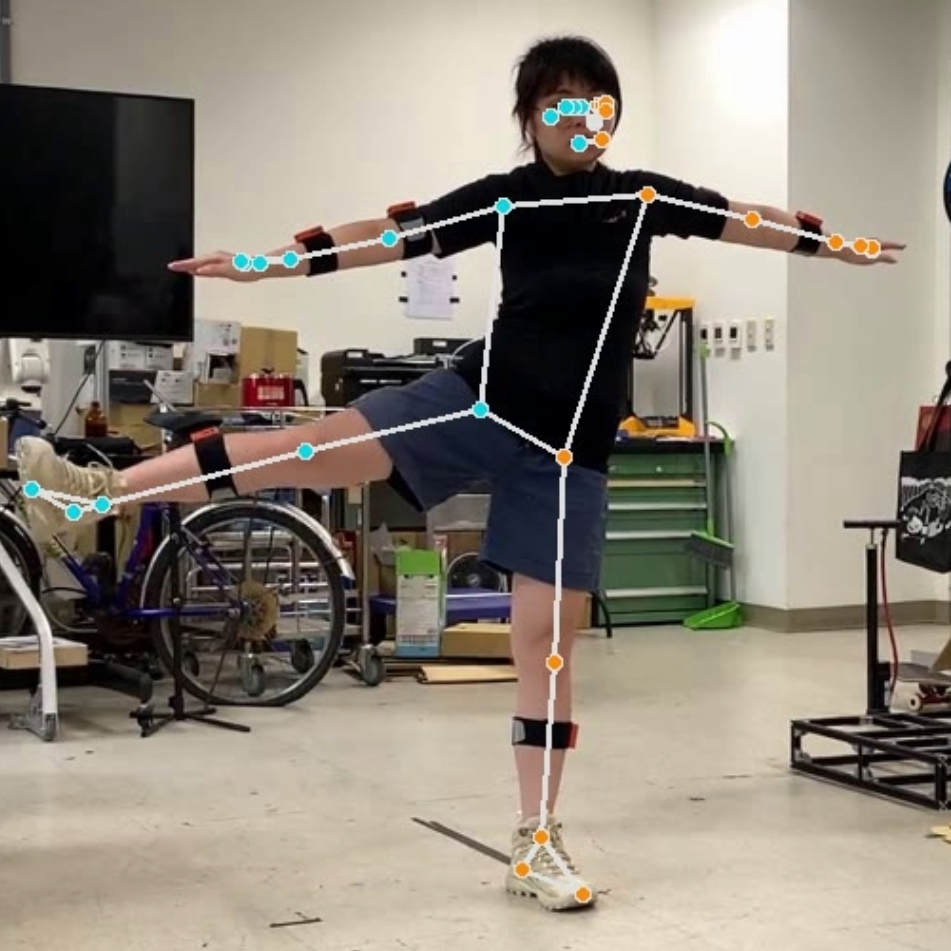
\includegraphics[width=\linewidth]{figure/ch2_fig_rec_mediapipe.png}
       \caption*{(b) MediaPipe}
    \end{minipage}
    \caption[影像辨識結果]{影像辨識結果}
    \label{ch2_fig_rec_result}
\end{figure}

\begin{figure}[!ht]
    \centering
    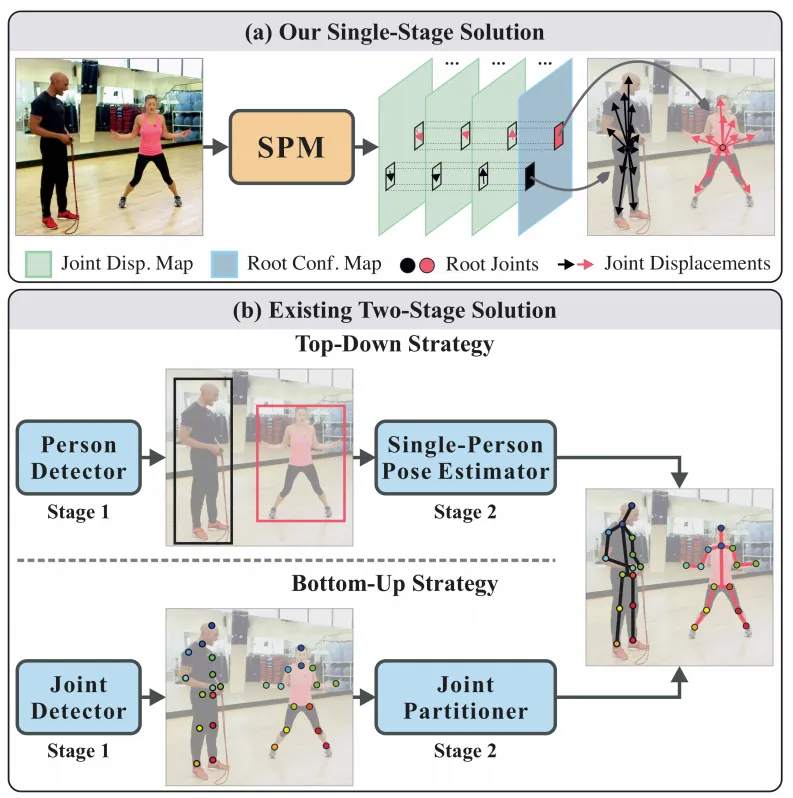
\includegraphics[width=11cm]{figure/ch2_fig_topvsbottom.png}
     \caption[辨識關節點位置的方法 ~\cite{nie2019single}]{辨識關節點位置的方法 ~\cite{nie2019single}}
     \label{ch2_fig_topvsbottom}
\end{figure}

\begin{figure}[!ht]
    \centering
    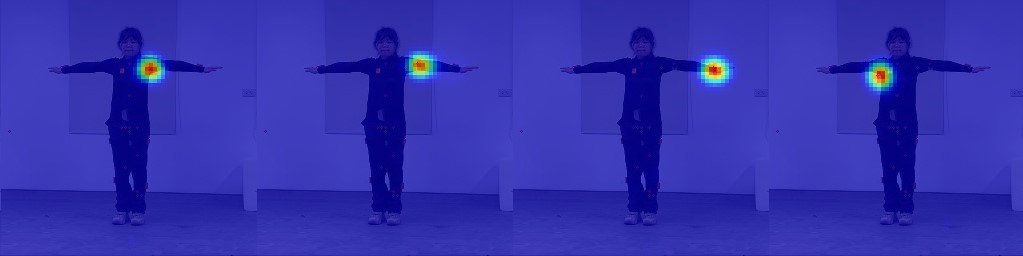
\includegraphics[width=\linewidth]{figure/ch2_fig_heatmap.jpg}
     \caption[影像辨識的輸出熱圖]{影像辨識的輸出熱圖}
     \label{ch2_fig_heatmap}
\end{figure}

\subsection{單感測器-慣性動作捕捉系統}
%  - IMU
    % - 只能量測到方向,無法量測到位置
    % - 量測時常拉長後會產生 drift 的問題
以朝向為主要量測目標的慣性動作捕捉系統,通常以可穿戴的慣性感測器 (Inertial Measurement Unit, IMU) 為量測工具,
一個測量單元包括加速規 (accelerometers)、陀螺儀 (gyroscopes) 及磁力計 (magnetometers) 三種感測器,
加速規用於測量三軸加速度,陀螺儀用於測量三軸角速度,磁力計用於測量三軸磁場強度,
透過三個感測器量得重力方向及地球磁場方向,
經由資料融合演算法推估出 IMU 當下的姿態~\cite{young2009comparison}~\cite{madgwick2011estimation}~\cite{nazarahari202140},
將 IMU 黏貼於欲量測的身體部位,例如頭部、手臂、腰部、腿等,即可量測受試者該部位的姿態。
現今最常被使用於量測人體姿態的 IMU 設備為 Xsens ~\cite{roetenberg2009xsens}~\cite{paulich2018xsens},
其使用無線傳輸技術傳遞量測資料,並可透過其提供的軟體進行各感測器間的時間與空間校正,
進而基於骨骼結構模型重建人體姿態~\cite{mcgrath2020body}~\cite{DIP:SIGGRAPHAsia:2018},如圖~\ref{ch2_fig_IMU_pose_estimate}所示,
更有學者進一步使用 IMU 的量測結果計算反向跳躍能力及骶骨運動學,以評估受試者的運動表現~\cite{mcginnis2016quantifying}~\cite{miranda2022accuracy},
或是使用 IMU 進行步態分析,用於評估步態障礙患者的康復情況~\cite{wang2020imu}~\cite{uchitomi2022three},如圖~\ref{ch2_fig_IMU_gait_estimate} 所示。

IMU 為一種微機電系統 (micro-electromechanical systems, MEMS) 感測器,
其功率消耗低、體積小、重量輕、攜帶方便,因此可量測場域廣泛,不受空間限制,可以作為日常配戴的裝置,時刻監測受試者的姿態;
且其可克服在無標記動作捕捉系統中的遮擋問題,及運動速度過快產生的模糊問題。
但是,IMU 僅可量測方向,無法量測位置,且隨著量測時間拉長,
將加速度進行積分後會產生嚴重的飄移問題 (drift),從而無法計算位置資訊;
且每次測量皆需校正每一感測器與其黏貼的身體部位的相對位置及相對方向,以確保量測結果的準確性,
在量測過程中,IMU 可能會因為肌肉出力與放鬆而有相對位置的變化,
進而影響量測結果的準確性~\cite{fiorentino2017soft}~\cite{stagni2005quantification}。

\begin{figure}[!ht]
    \centering
    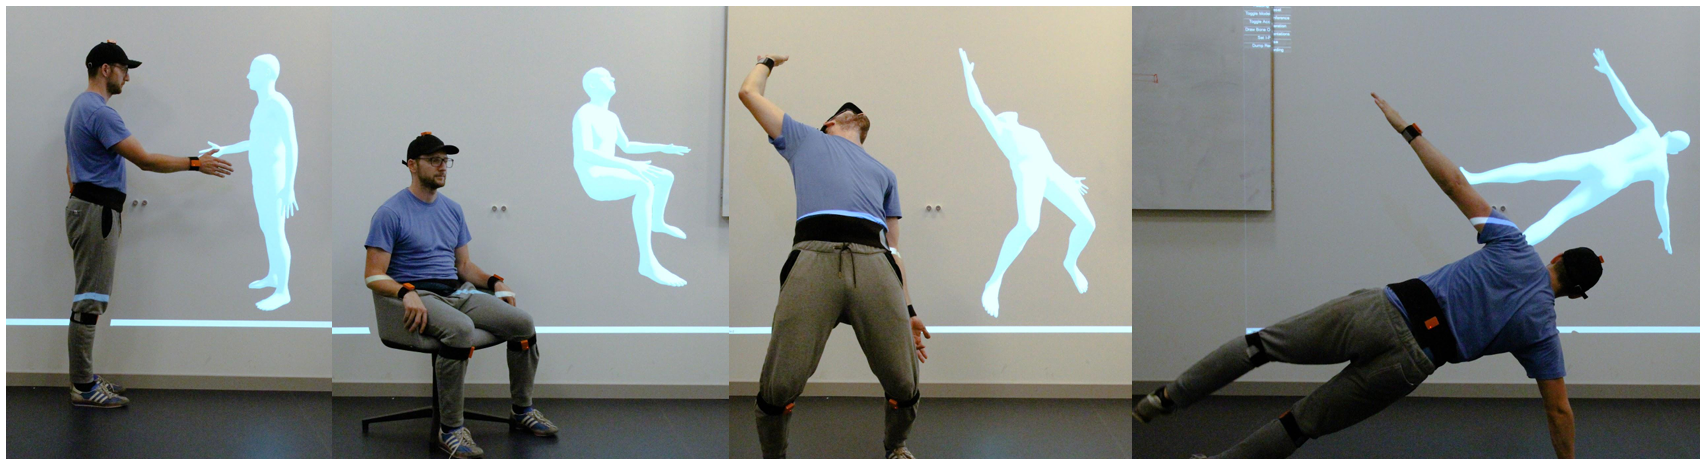
\includegraphics[width=\linewidth]{figure/ch2_fig_IMU_pose_estimate.png}
     \caption[使用 IMU 重建人體姿態]{使用 IMU 重建人體姿態}
     \label{ch2_fig_IMU_pose_estimate}
\end{figure}

\begin{figure}[!ht]
    \centering
    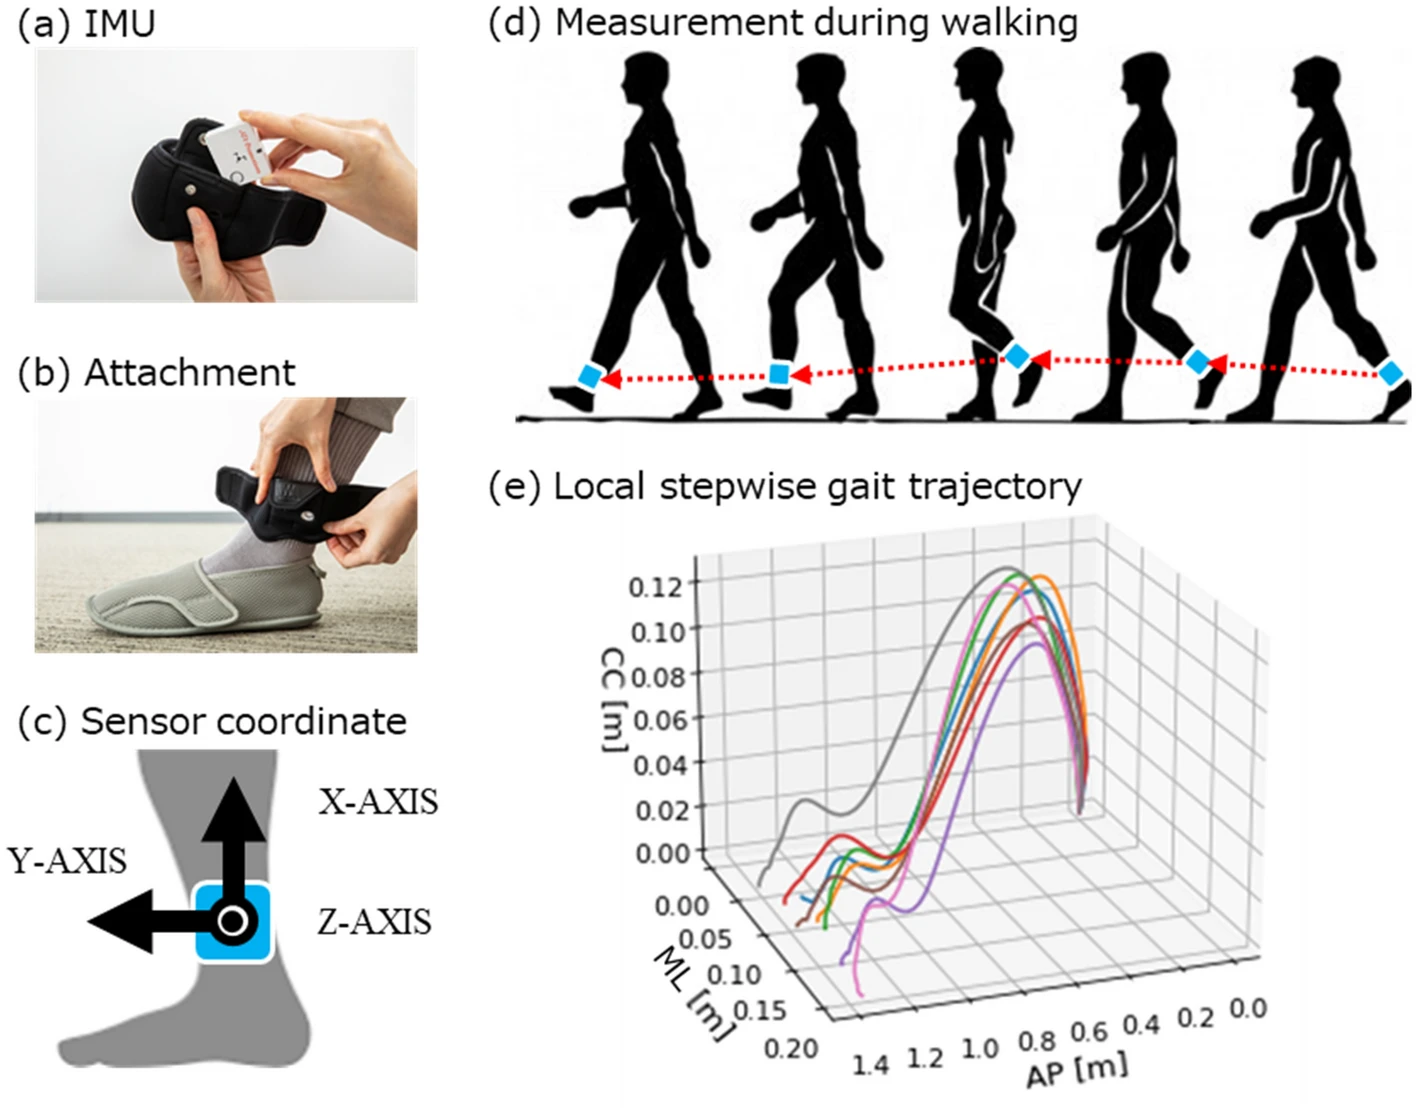
\includegraphics[width=\linewidth]{figure/ch2_fig_IMU_gait_estimate.png}
     \caption[使用 IMU 進行步態分析]{使用 IMU 進行步態分析}
     \label{ch2_fig_IMU_gait_estimate}
\end{figure}

\subsection{多感測器融合動作捕捉系統}
% - 相機與 IMU 融合
% - 3DPW、totalcapture、real-time full-body…、wearable fusing…
由於無標記光學動作捕捉系統會因為遮擋問題而無法辨識出被遮擋的關節,IMU 量測時長拉長會產生飄移問題,
因此,學者們開始將光學動作捕捉系統與 IMU 進行融合,以彌補各自的缺點~\cite{li2023visual},
藉由 IMU 的量測資料補足光學動作捕捉系統的遮擋、移動快速產生模糊的問題,
並藉由光學動作捕捉系統不受磁場影響的特性,解決 IMU 量測時長拉長產生飄移的問題,同時可用於計算受試者於空間中的位置資訊。

多感測器融合方法可應用於自動駕駛、智慧機器人、增強實境 (AR) 及虛擬實境 (VR) 等領域~\cite{jinyu2019survey}~\cite{zhu2023camera},
也可應用於人體動作捕捉領域,人體動作捕捉範圍可包含手部、上半身、下半身、全身等不同部位,
例如 Matthew Trumble 等人使用 4 或 8 台相機及 13 個 IMU 進行融合,建立人體全身姿態,
並發表一系列經過時間對齊的多視角影片 (multi-viewpoint video, MVV) 搭配 IMU 資料集~\cite{Trumble:BMVC:2017};
或如學者 Zhe Zhang 等人使用 TotalCapture 資料集中的 4 台攝影機,及 8 個 IMU 資料融合,
並使用同資料集的 Vicon 資料驗證融合方法,誤差為 24.6 (mm) ~\cite{Zhang_2020_CVPR};
又如學者 Von Marcard 等人提出的 3DPW ~\cite{vonMarcard2018},
使用一台手持式可移動相機及 6 \textasciitilde\ 17 個 IMU 融合重建人體在戶外運動的姿態,如圖~\ref{ch2_fig_3DPW} 所示,
使用 TotalCapture 資料集驗證融合方法,誤差為 26 (mm),並發表一系列可供下載的資料集。
% TODO:想加上下半身的研究
相機及 IMU 使用數量可有多種組合,端看學者們的需求及實驗設計。

\begin{figure}[!ht]
    \centering
    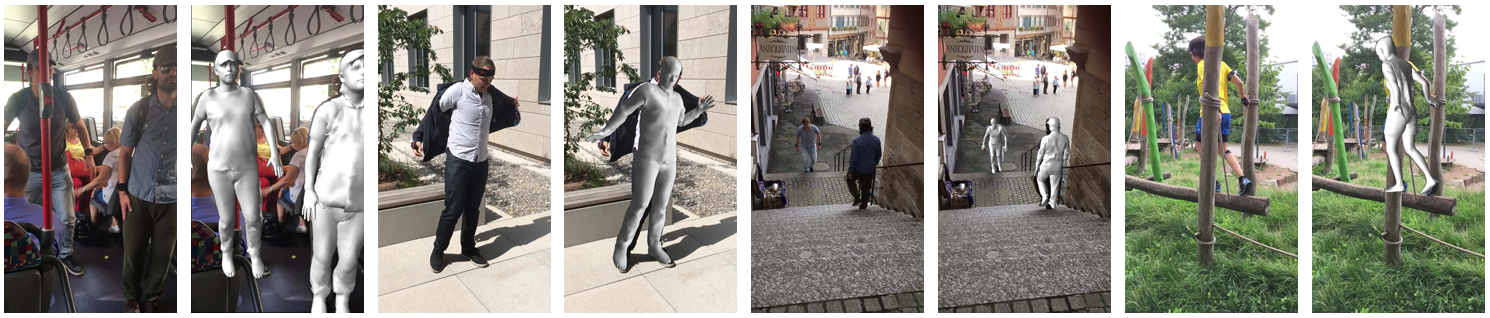
\includegraphics[width=\linewidth]{figure/ch2_fig_3DPW.png}
     \caption[多感測器融合建立人體姿態]{多感測器融合建立人體姿態}
     \label{ch2_fig_3DPW}
\end{figure}

% ------------------------- 2.2 ------------------------- %
\section{個人化人體模型}
% 個人化骨架,還沒頭緒要寫什麼
% - 可能可以提及前人的做法,例如使用 Vicon 作為骨架,但是這樣的骨架不夠個人化,所以我要做這些事情
在人體姿態估計領域,使用動作捕捉系統過程中,通常會參考人體模型的骨架結構及物理限制,以避免估計出不符合人體結構的姿態,
動作捕捉系統建立人體姿態後,常會使用人體模型 (human body model) 來描述與表示受試者的姿態,
因此需建立一個個人化的人體模型,其符合受試者的骨架結構、體型及物理限制,以提高姿態估計的準確性,
人體模型可用於描述人體結構、人體形狀及人體表面紋理等資訊~\cite{gong2016human}。
依照模型包含的資訊不同,人體模型可分為運動學模型 (Kinematic model)、平面模型 (Planar Model)、體積模型 (Volumetric Model) 三類,
如圖~\ref{ch2_fig_personal_model} 所示。

\begin{figure}[!ht]
    \centering
    \begin{minipage}{.33\textwidth}
       \centering
       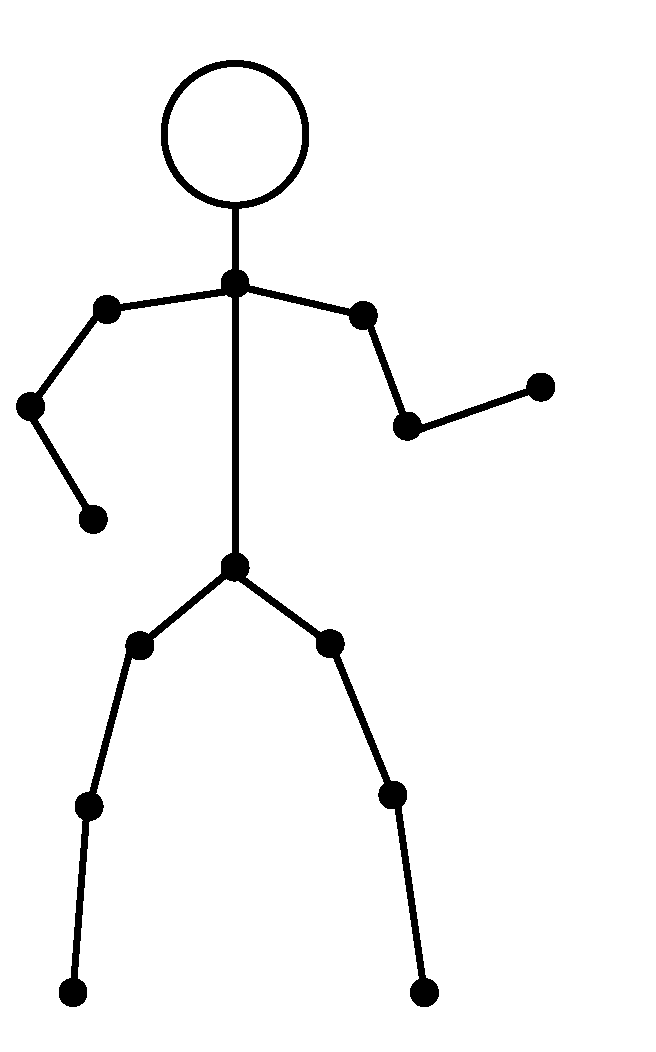
\includegraphics[width=\linewidth]{figure/ch2_fig_personal_kinematic_model.png}
       \caption*{(a) 運動學模型}
    \end{minipage}%
    \begin{minipage}{.33\textwidth}
       \centering
       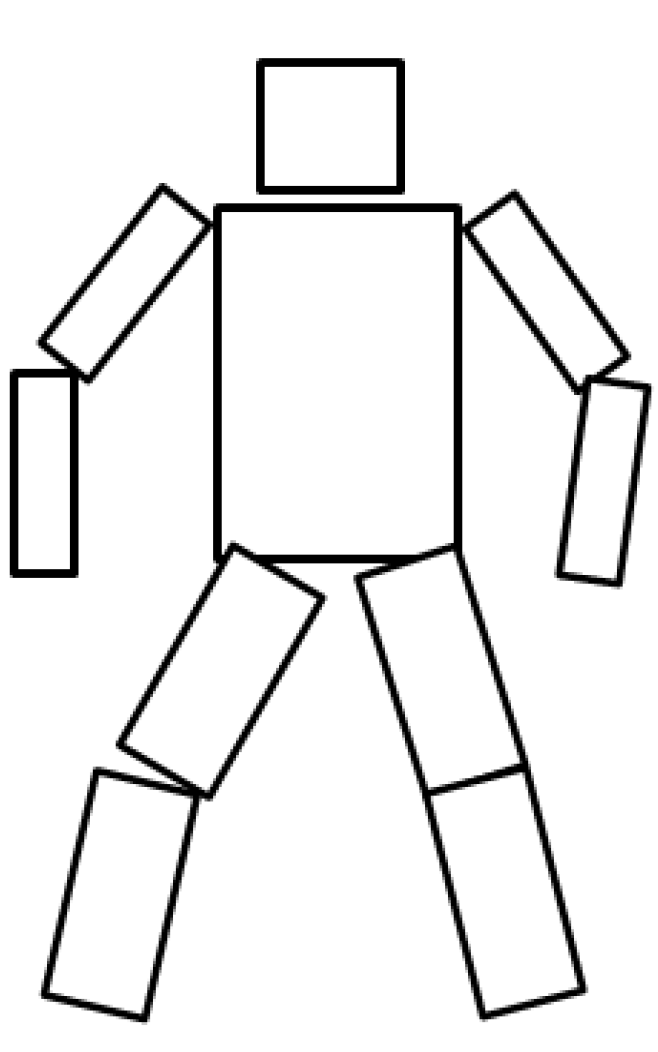
\includegraphics[width=\linewidth]{figure/ch2_fig_personal_volumetric_model.png}
       \caption*{(b) 平面模型}
    \end{minipage}%
    \begin{minipage}{.33\textwidth}
      \centering
      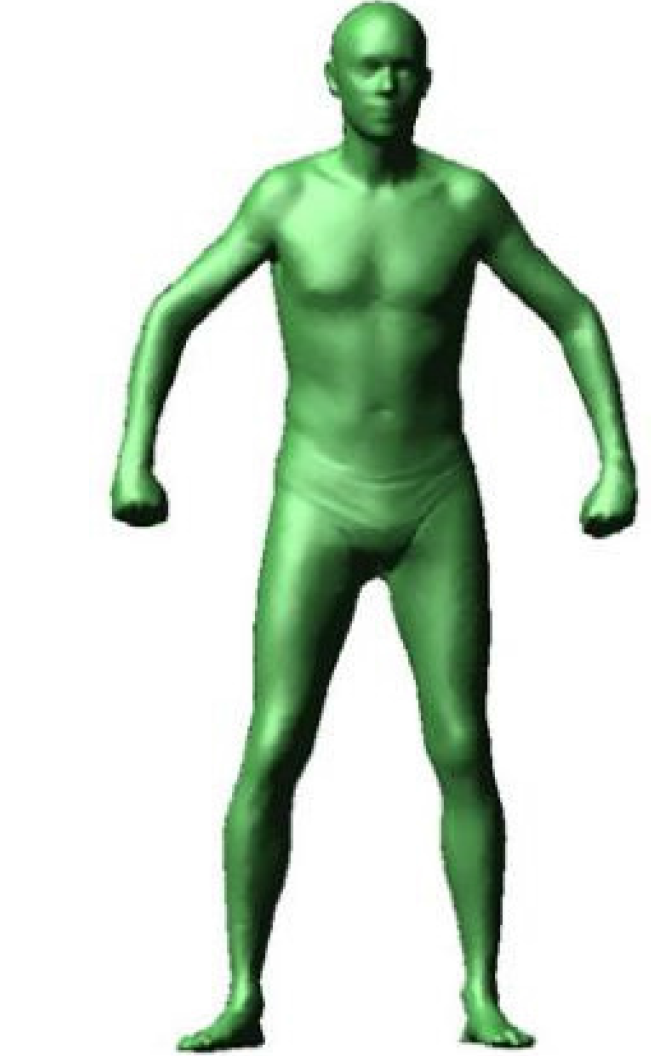
\includegraphics[width=\linewidth]{figure/ch2_fig_personal_planar_model.png}
      \caption*{(c) 體積模型}
    \end{minipage}
    \captionsetup{justification=centering}
    \caption[三種人體模型]{三種人體模型}
    \label{ch2_fig_personal_model}
 \end{figure}

\subsection*{運動學模型}
運動學模型是最常見且最頻繁被應用的模型,可用於描述二維或三維人體姿態,
通常只考慮人體骨架結構,不考慮人體的肌肉組織,以點描述關節位置,並以棍子連接關節,代表人體指定肢體的骨骼方向,
因此運動學模型可以淺顯易懂的方式描述人體部位間的關係,但無法描述人體的形狀及表面紋理。

運動學模型可分為兩類,一類為預定義模型 (predefined model),另一類為學習圖像結構模型 (learned graph structure model)。
預定義模型結構為基於人體解剖學與物理定義所建構,其關節點名稱、層級與父子關係皆有既定定義,
不受動作捕捉數據影響,不涉及任何機器學習過程,例如 Vicon 系統中的骨架結構。
除 Vicon 系統的骨架結構外,也有學者使用預定義模型描述人體姿態估計,例如 DeepPose ~\cite{Toshev_2014_CVPR},
或是基於預定義模型進行機器學習,以約束結果符合人體結構~\cite{wei2016convolutional}。
預定義模型具有明確的物理意義,且易於解釋,但模型結構較為簡化,因此無法捕捉複雜且具有細節的運動模式。

學習圖像結構模型則從大量的人體運動圖像數據中學習人體的結構,從而建構起人體的模型,
學習圖像結構模型的方法十分多樣,一種最為常見的模型為圖像結構模型 (Pictorial Structure Models, PSM)~\cite{johnson2010clustered},
學習圖像模型可以捕捉複雜的運動模式,具有較好的人體描述能力,且模型可從數據中學習到更多的特徵,減少人工設計的成分,
但模型結構較為複雜,且可能缺乏明確的物理意義,因此難以解釋。

\subsection*{平面模型}
平面模型則是將人體分割成多個平面,以平面描述人體的外觀及形狀,
身體各部位由與人體部位相似的矩形組成,可被用於描述二維人體姿態,
例如 Active Shape Model (ASM),其使用主成分分析方法 (principal component analysis, PCA) 取得完整的人體形狀及輪廓,
以表示人體全身姿態~\cite{freifeld2010contour}。平面模型由於組成比體積模型簡單,因此計算速度較快,
但是因為只能描述二維人體姿態,缺乏深度資訊,因此對於複雜的三維人體姿態描述能力較差。

\subsection*{體積模型}
體積模型包括人體的形狀資訊,人體部位由相似形狀的圓柱體或圓錐體描述,圓柱體或圓椎體間的接點即為關節,
或是使用數千個網格組成人體表面,形成人體體積模型,可被用於描述三維人體姿態,模型的樣貌最接近人體型態,
例如學者 Matthew Loper 等人提出的 SMPL 模型 (Skinned Multi-Person Linear model)~\cite{SMPL:2015},
SMPL 模型為一款開源的人體體積模型,由 23 個關節及 6890 個網格頂點組成,可用於描述人體的形狀及姿態,
體積模型可以描述人體的形狀及表面紋理,且具有較好的人體描述能力,但是模型結構較為複雜,且計算速度較慢。

% ------------------------- 2.3 ------------------------- %
\section{時間對齊}
% 時間對齊的重要性
感測器間皆有各自的計時器及採樣頻率,因此無論是使用同類型感測器或是使用並融合不同類型的感測器,皆需考慮使用的資料點是否位於相同的時刻,
若資料點不在相同時刻,則需進行時間對齊 (time synchronization) 的處理,以確保資料點的一致性。
最常見的時間對齊方法,一為使用硬體觸發器,透過硬體觸發器同時觸發所有感測器進行採樣,確保所有感測器的資料點位於相同時刻;
二為使用預先定義的動作進行時間對齊,
例如使用拍手動作,透過拍手發出的聲音進行影像間的時間對齊,
再透過拍手時巨大的加速度變化進行 IMU 與影像間的時間對齊~\cite{pons2012data};
或是使用垂直跳躍或跺腳等動作,透過動作開始的時間點進行影像對齊,
再透過動作中的加速度變化對齊 IMU 與影像的時間~\cite{destelle2014low}~\cite{Trumble:BMVC:2017};
抑是直接使用受試者的動作進行時間對齊,例如直接尋找影像中受試者走路時腳與地面接觸的時間點,
在影像方面,可以直接從影像辨識到的踝關節運動進行推測,
在 IMU 方面,可透過貼於腳上的 IMU 的加速度測量值中計算出腳與地面接觸的時間點~\cite{kaichi2020resolving};
也可使用 LED 燈及遠紅外光 LED 燈進行時間對齊,透過 LED 燈的閃爍進行影像間的時間對齊~\cite{nakano2020evaluation}~\cite{needham2021accuracy}。
上述之時間對齊方法,皆有對應適合的感測器,因此在選擇時間對齊方法時,需依照研究需求進行選擇。

% ------------------------- 2.4 ------------------------- %
\section{感測器融合演算法}
% 感測器融合演算法
使用多種不同感測器量測人體姿態,其資料間可能存在不同的誤差或雜訊,因此需進行感測器融合 (sensor fusion) 處理,
感測器融合方法可依照融合層級分類為原始資料層級融合 (Raw Data-Level Fusion)、特徵層級融合 (Feature-Level Fusion)、
決策層級融合 (Decision-Level Fusion) ~\cite{majumder2020vision};
也可依照融合演算法分類為直接融合方法 (Deterministic Method)、濾波融合方法 (Filter-Based Methods)、
最佳化融合方法 (Optimization-Based Methods)、機器學習融合方法 (Learning-Based Methods) ~\cite{li2023visual}。

% TODO:猶豫要不要把層級融合的圖放上去,如果要放應該是放層級融合那篇的 fig3

\subsection*{直接融合方法}
% 直接融合方法 (Deterministic Method) 使用簡單的邏輯計算或是加權平均計算,不涉及複雜的模型或算法,
% 將多個感測器的資料直接合併得到最終的姿態估計。
直接融合方法 (Deterministic Method) 屬於決策層級融合,
在執行直接融合前,無標記光學動作捕捉系統及慣性動作捕捉系統皆已完成數據蒐集、特徵提取、姿態估計,
直接融合方法僅將兩者的結果進一步進行邏輯計算或是加權平均,得到最終的姿態估計,
不涉及複雜的模型或算法,也不涉及原始數據的修正及是否提取特定特徵的判斷。
例如學者 Masataka Yamamoto 等人為了提高人體踝關節角度的估計準確度,
將慣性動作捕捉系統的加速度及角加速度數據與無光標記動作捕捉系統數據使用互補濾波器進行融合~\cite{yamamoto2022verification};
又如學者 Grzegorz Glonek 等人,分別計算出兩種捕捉系統的軸關節角度,
並依無光標記動作捕捉系統的關節狀態是否可見,決定其結果是否可靠,從而決定兩者的融合權重~\cite{s17122857}。

直接融合方法的優點為計算簡單直接,不需要複雜的模型及冗長的計算,但是每一種量測方法都存在誤差及雜訊,
直接融合方法沒有對誤差及雜訊進行處理,將這些誤差及雜訊也一併進行融合,因此可能會導致融合結果不夠準確。

\subsection*{濾波融合方法}
在需要即時處理多模態且帶有雜訊的感測器數據時,濾波融合方法 (Filter-Based Methods) 是一種常見的原始資料層級融合方法,
在執行濾波融合時,輸入通常是 IMU 的原始加速度、角速度及影像的特徵點座標,融合過程中直接對原始資料進行濾波處理,估計人體姿態。
較常被使用的濾波器包括卡爾曼濾波器 (Kalman Filter)、擴展卡爾曼濾波器 (Extended Kalman Filter)、無迹卡爾曼濾波器 (Unscented Kalman Filter),
例如學者 S. M. Orozco-Soto 等人,使用卡爾曼濾波器融合 IMU 資訊及影像資訊,估計受試者的上肢關節角度~\cite{orozco2019development},
又如學者 Randa Mallat 等人,使用擴展卡爾曼濾波器融合 IMU 資訊及影像資訊,估計受試者的上肢關節角度,
藉此評估人類上肢康復過程中的活動能力~\cite{mallat2020upper}。

濾波融合方法可以對原始資料進行濾波處理,去除雜訊及誤差,提高融合結果的準確性,且計算複雜度低,可以及時估計人體姿態,
但是濾波融合方法需要對濾波器進行參數調整,需要有準確的模型及參數,否則模型誤差可能會影響融合結果的準確性。

\subsection*{最佳化融合方法}
% 最佳化融合方法 (Optimization-Based Methods) 取決於輸入資訊決定其為原始資料融合、特徵層融合或是決策層融合,
在執行最佳化融合方法 (Optimization-Based Methods) 前,無標記光學動作捕捉系統及慣性動作捕捉系統皆已完成數據蒐集、特徵提取,
透過建立最佳化模型,將兩者的特徵透過目標函數、限制條件進行最佳化,得到最終的姿態估計。
如學者 Charles Malleson 等人,透過建立包含朝向項、位置項、加速度項等項次的目標函數,
並使用 Ceres non-linear least-squares solver 計算目標函數的最佳解,從而估計人體全身姿態~\cite{malleson2017real},
又如學者 Ahmed Ahmed 等人,使用批次最小平方法 (batch least-squares algorithm, BLS) 進行最佳化,
融合兩個黏貼於雙腳的 IMU 及頭戴式 IMU 相機,並使用不同行走狀態對應的運動約束,
以估計受試者頭部與腳部的姿勢,從而估計受試者的步態~\cite{ahmed2018visual}。

最佳化融合方法透過建立目標函數及多項限制條件的方式,將 IMU 與影像的特徵進行最佳化融合,
且可以根據不同的應用場景及需求,建立不同的目標函數及限制條件,提高融合結果的準確性;
但最佳化求解過程需要較長的計算時間及大量的計算資源,且有一些最佳化演算法可能會陷入局部最佳解的誤區,而無法找到全局最佳解。

\subsection*{機器學習融合方法}
機器學習融合方法 (Learning-Based Methods) 透過機器學習的方式,
從人工標註的數據學習將 IMU 與影像的相關資訊進行融合,並建立模型,從而估計人體姿態。
例如學者 Matthew Trumble 等人,使用長短期記憶網路 (Long Short-Term Memory, LSTM) 處理關節位置估計值,
並與 IMU 相關資訊融合,得到最終人體全身估計姿態~\cite{Trumble:BMVC:2017}。
% 又如學者 Young-Woon Cha 等人,使用深度學習方法,將 IMU 與影像的特徵進行融合,
% TODO:另一個例子有空再回來寫好了,現在有點寫不下去QQ

機器學習融合方法有強大的學習能力,可以自動從原始數據開始進行特徵提取及融合,無需人工進行資料前處理或後處理,
並且可以根據不同的應用場景及需求,建立不同的模型,靈活性較高;
但是在訓練過程中,需要大量的人工標註資料,人工標註資料的準確性將直接影響模型的準確性,
同時,訓練模型需要大量的訓練參數,因此計算成本高,
且模型的解釋性較差,難以解釋模型的輸出結果。

% ------------------------- 2.5 ------------------------- %
\section{小結}
描述目前文獻不足的地方,所以我要做這些事情
我的部分可能就是描述目前使用的文獻都是使用 Vicon 作為骨架,我想要改善這一點,還有資料對其的地方,要再思考這不分要如何在前面2.3的章節先提到,而且可以承接章節2.2

- 骨架
- 時間對齊

% 章節回顧;個人化模型必要
本章節回顧了與研究主題相關的論文,首先從最基礎的量測技術開始介紹,
像是動作捕捉系統、力感測裝置與 EMG 等常見的量測方法,這些儀器能夠量化人體的動作表現,
透過數據處理針對特定主題來深入探討,亦可作為模擬的輸入或是輸出的驗證比較,其中量測的精準度將對應用有大幅影響,
因此在校正量測結果或是提高估計準確度上皆是重要的議題;接續介紹關於人體動作模擬的工作流程、系統、模型,
以及相關的研究文獻,研究探討不再僅限於臨床實驗當中,另外像是肌肉力量、關節扭矩等這些難以量測的資訊,
皆可在電腦中快速地取得,獲取資訊的種類增加意味著能探討的問題更加多元,大幅增廣在生物力學上的觀點;
最後針對個人化模型議題進行更深入的調查,模型準確度代表著與受試者是否有密切關聯,若僅透過通用模型進行研究,
模擬結果將與實際情況有所落差,而個人化模型能對所感興趣的資訊更真實的呈現,
因此根據不同受試者來建立對應的個人化模型是必要的。

% 重述困境;誤差是否可接受;肌肉代償;參數抗衡
個人化模型的建立將會複雜許多,以肌肉參數為例,除了參數取得不易外,還有可能會發生肌肉代償問題,
而在同一條肌肉的參數間,其亦具有參數不可識別性,在運動軌跡預測作為驗證的文獻中,
於比較軌跡的圖形裡 (文獻 Fig. 6),這個量級的誤差是否為可接受的?在肌肉代償與參數間會互相抗衡的情況下,
微小的誤差就會造成參數的估計錯誤,若誤差大到一定程度,其評估效果也將不及通用模型,
故在估計與驗證參數的過程是十分重要的。

% 論文重點;章節安排
本論文著重在肌肉參數的估計中,對於上述的問題進行深入探討與驗證,提出一套適用的估計參數研究方法,
並以已建立好的上肢模型作為驗證,除了進行參數估計外,也會呈現參數間抗衡的範例,來顯現該問題的重要性。

\clearpage
\chapter{研究方法}
\fontsize{12pt}{18pt}\selectfont

% ------------------------- 3.0 ------------------------- %
% 研究目的;研究假設;研究方法
本研究目的是透過最佳化方法估計肌肉參數,省去醫療器材量測之高成本,藉以生成個人化模型,
應用於復健規劃、運動訓練與輔具設計等領域。本研究假設為已知一肌肉骨骼模型,該模型除了欲評估之肌肉參數外,
其餘幾何特徵、肌肉參數等資訊皆為已知,而其可透過 OpenSim 軟體來執行任何模擬。研究方法主要分為三大主軸,
介紹如下:
\begin{itemize}
    \item \textbf{主軸一:敏感度分析}
    \\ 透過擾動肌肉參數,來計算出任務與參數間之敏感度,其指標是藉由預測任務之誤差來表示。
       敏感度高意味著該肌肉和該任務具有高相關性,其結果提供最佳化與模型驗證之任務挑選的參考依據。
    \item \textbf{主軸二:多運動軌跡預測最佳化}
    \\ 從敏感度分析挑選數個適當任務作為輸入,並將多運動軌跡預測任務之平均預測誤差視作目標函數,
       藉由最佳化方法最小化平均預測誤差,以此估計出最佳模型之肌肉參數。   
    \item \textbf{主軸三:模型驗證}
    \\ 從敏感度分析挑選適當任務作為輸入,指定最佳模型完成並檢視其預測誤差,
       確認該模型是否於其它任務仍具有低誤差表現,以此驗證模型正確性。
\end{itemize}

% 研究流程圖 + 說明
本研究之流程圖如圖 所示,首先輸入標準模型和分析參數來執行敏感度分析,
藉由全因子實驗設計法來評估出所有任務之敏感度指標,接下來挑選適合的組合集作為最佳化之評估任務,
以生成最佳模型,最終透過高敏感度任務進行模型驗證,來評估最佳模型之正確性。
若於模型驗證階段成功,代表評估正確,並結束程式執行;若於模型驗證階段失敗,則返回至最佳化步驟重新評估;
若模型驗證失敗次數過多,則返回至敏感度分析流程,重新挑選合適的評估任務。
程式碼將發布於 https://github.com/solab-ntu/MuscleParamEstimation 該網址中,執行細節可檢視程式碼中的註解說明。

\clearpage

% ------------------------- 3.1 ------------------------- %
\section{實驗系統設定與實驗環境}\label{ch3_exp_setting}
% 系統架設;實驗環境
% 說明會講到實驗流程、系統設定、實驗環境等等的事情
進行人體姿勢估計的實驗,需要使用多種感測器來量測人體姿態,且需要多項事情準備工作及設置,
本章節將會依序說明整體實驗流程、實驗系統設定、實驗環境及實驗動作。

\subsection{實驗流程}
% 講我蒐集資料的事前工作,和整個流程的概述
在進行人體姿態估計的實驗流程如圖~\ref{ch3_fig_exp_flow} 所示,
首先進行相機內部參數及外部參數拍攝,
拍攝內部參數影片時,需使棋盤格校正板盡可能填滿畫面,並涵蓋多種不同角度的畫面,以便進行內部參數的計算,
拍攝外部參數影片時,需由受試者站在實驗初始位置並拿著棋盤格校正板,以便進行外部參數的計算。
接著進行人體骨架資料搜集,
由受試者站在實驗初始位置,進行時間對齊動作後,維持 T 姿勢約 1~2 秒進行拍攝及 IMU 量測,最後再進行一次時間對齊動作,
完成人體骨架資料搜集。
再來即可開時進行實驗動作資料搜集,
由受試者站在實驗初始位置,進行時間對齊動作後,進行實驗動作拍攝及 IMU 量測,最後再進行一次時間對齊動作,
完成實驗動作資料搜集。
實驗資料搜集到此告一段落,接著將搜集到的影像資料及 IMU 量測資料進行時間對齊、空間對齊,並進行感測器融合,
輸出即為立體人體姿態估計結果,最後進行肢段長度計算進行驗證。

\begin{figure}[!ht]
   \centering
   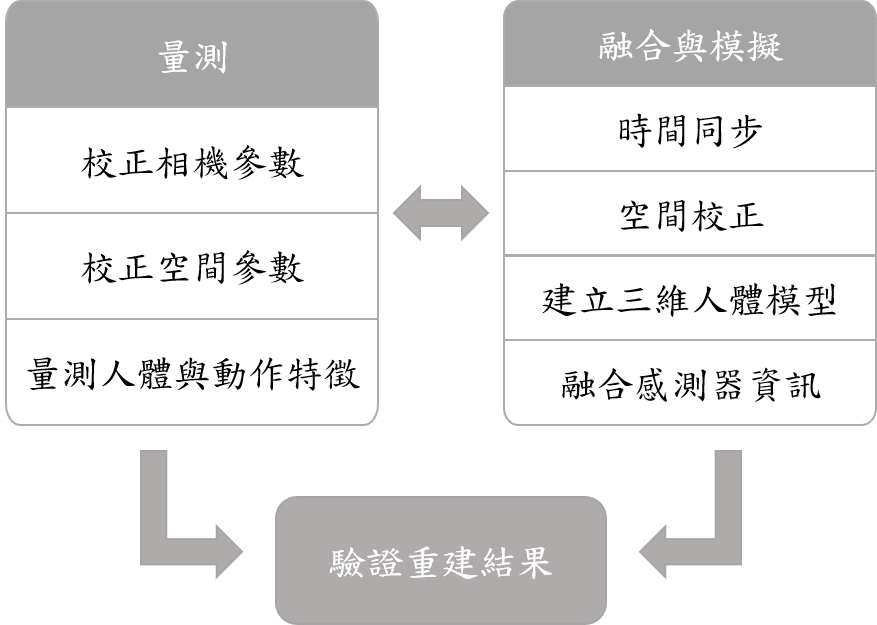
\includegraphics[width=\linewidth]{figure/ch3_fig_exp_flow.png}
    \caption[人體姿態估計實驗流程]{人體姿態估計實驗流程}
    \label{ch3_fig_exp_flow}
\end{figure}

\subsection{實驗系統設定}
% 系統架設介紹
% 實驗設定:T pose、拍手等等姿勢
% 說明我這一段要講我用了哪些工具的前言
本研究用於量測人體姿態的工具包含兩台 iPhone 手機、Xsens、棋盤格校正板,各自的功能如下:
兩台手機用於記錄人體姿態的影像資料,擺放於特定位置,拍攝受試者的全身影像;
Xsens 用於記錄人體各肢段及棋盤格校正板的朝向資訊,共使用 10+1 顆 IMU 進行量測;
棋盤格校正板用於轉換影像座標系至全域座標系,以建立影像座標系與全域座標系間的關係。
另外,需要求受試者穿著黑色長袖上衣及黑色長褲,長度盡可能遮蓋住手腕及腳踝。


\subsubsection{位置資訊量測工具 - 相機及擺放位置}
% 硬體介紹;使用相機及擺放位置(平面圖和受試者的移動範圍,用上視表示),幀率(frame rate)為 60 Hz,校正板規格、黑色長秀長庫
% 擺放位置這邊可能會說在後面實驗環境章節再詳細說明
本研究使用兩支 iPhone 手機進行影像資料量測,分別為 iPhone XR 及 iPhone 15 Pro,皆以主鏡頭錄影格式進行拍攝,
拍攝過程不使用縮放功能,僅使用手機本身的鏡頭進行拍攝,
兩支手機皆設定影像擷取畫面為 1920x1080,幀率設定為 60 Hz。

本研究將 iPhone XR 編號為 cam01,將 iPhone 15 Pro 編號為 cam02,
手機擺放位置如圖所示,cam01 拍攝高度為 79 (cm),cam02 拍攝高度為 74 (cm),
在實驗資料搜集過程中,拍攝角度及位置皆維持不變。
% TODO:補相機在空間中的位置圖(簡略的畫一下空間尺度就好,詳細的尺度放在室內實驗環境及尺寸)

\subsubsection{朝向資訊量測工具 - Xsens}
% 軟體介紹;xsens,講使用的軟體 MT manager 還有分析出朝向和加速度應用的模型(在 MT manager),採樣率60HZ
% 還有用了幾顆 IMU ,分別擺在身體的哪裡,要寫身上和板子上的擺放位置和方向
本研究使用 Xsens 提供之硬體及軟體 MT-manager 作為量測姿態朝向的工具,採樣率設定為 60 Hz,共使用 10+1 顆 IMU 進行量測,
十顆 IMU 分別黏貼於左右上臂中段外側、左右手腕外側、胸骨、骨盆、左右大腿中段外側、左右小腿中段外側,共十處,
如圖~\ref{ch3_fig_humanimu} 所示, IMU 長軸 (即 x 軸) 與骨頭長度方向對齊,隨時間進行搜集各時間點受試者各肢段的朝向資訊。
另一顆 IMU 黏貼於棋盤格校正板,量測棋盤格校正板的初始朝向,用以轉換影像座標系至全域座標系,如圖~\ref{ch3_fig_cbimu} 所示,
IMU 的 x、y 軸對齊棋盤格校正板的 x、y 座標方向。

\begin{figure}[!ht]
   \centering
   \begin{minipage}{.25\textwidth}
     \centering
     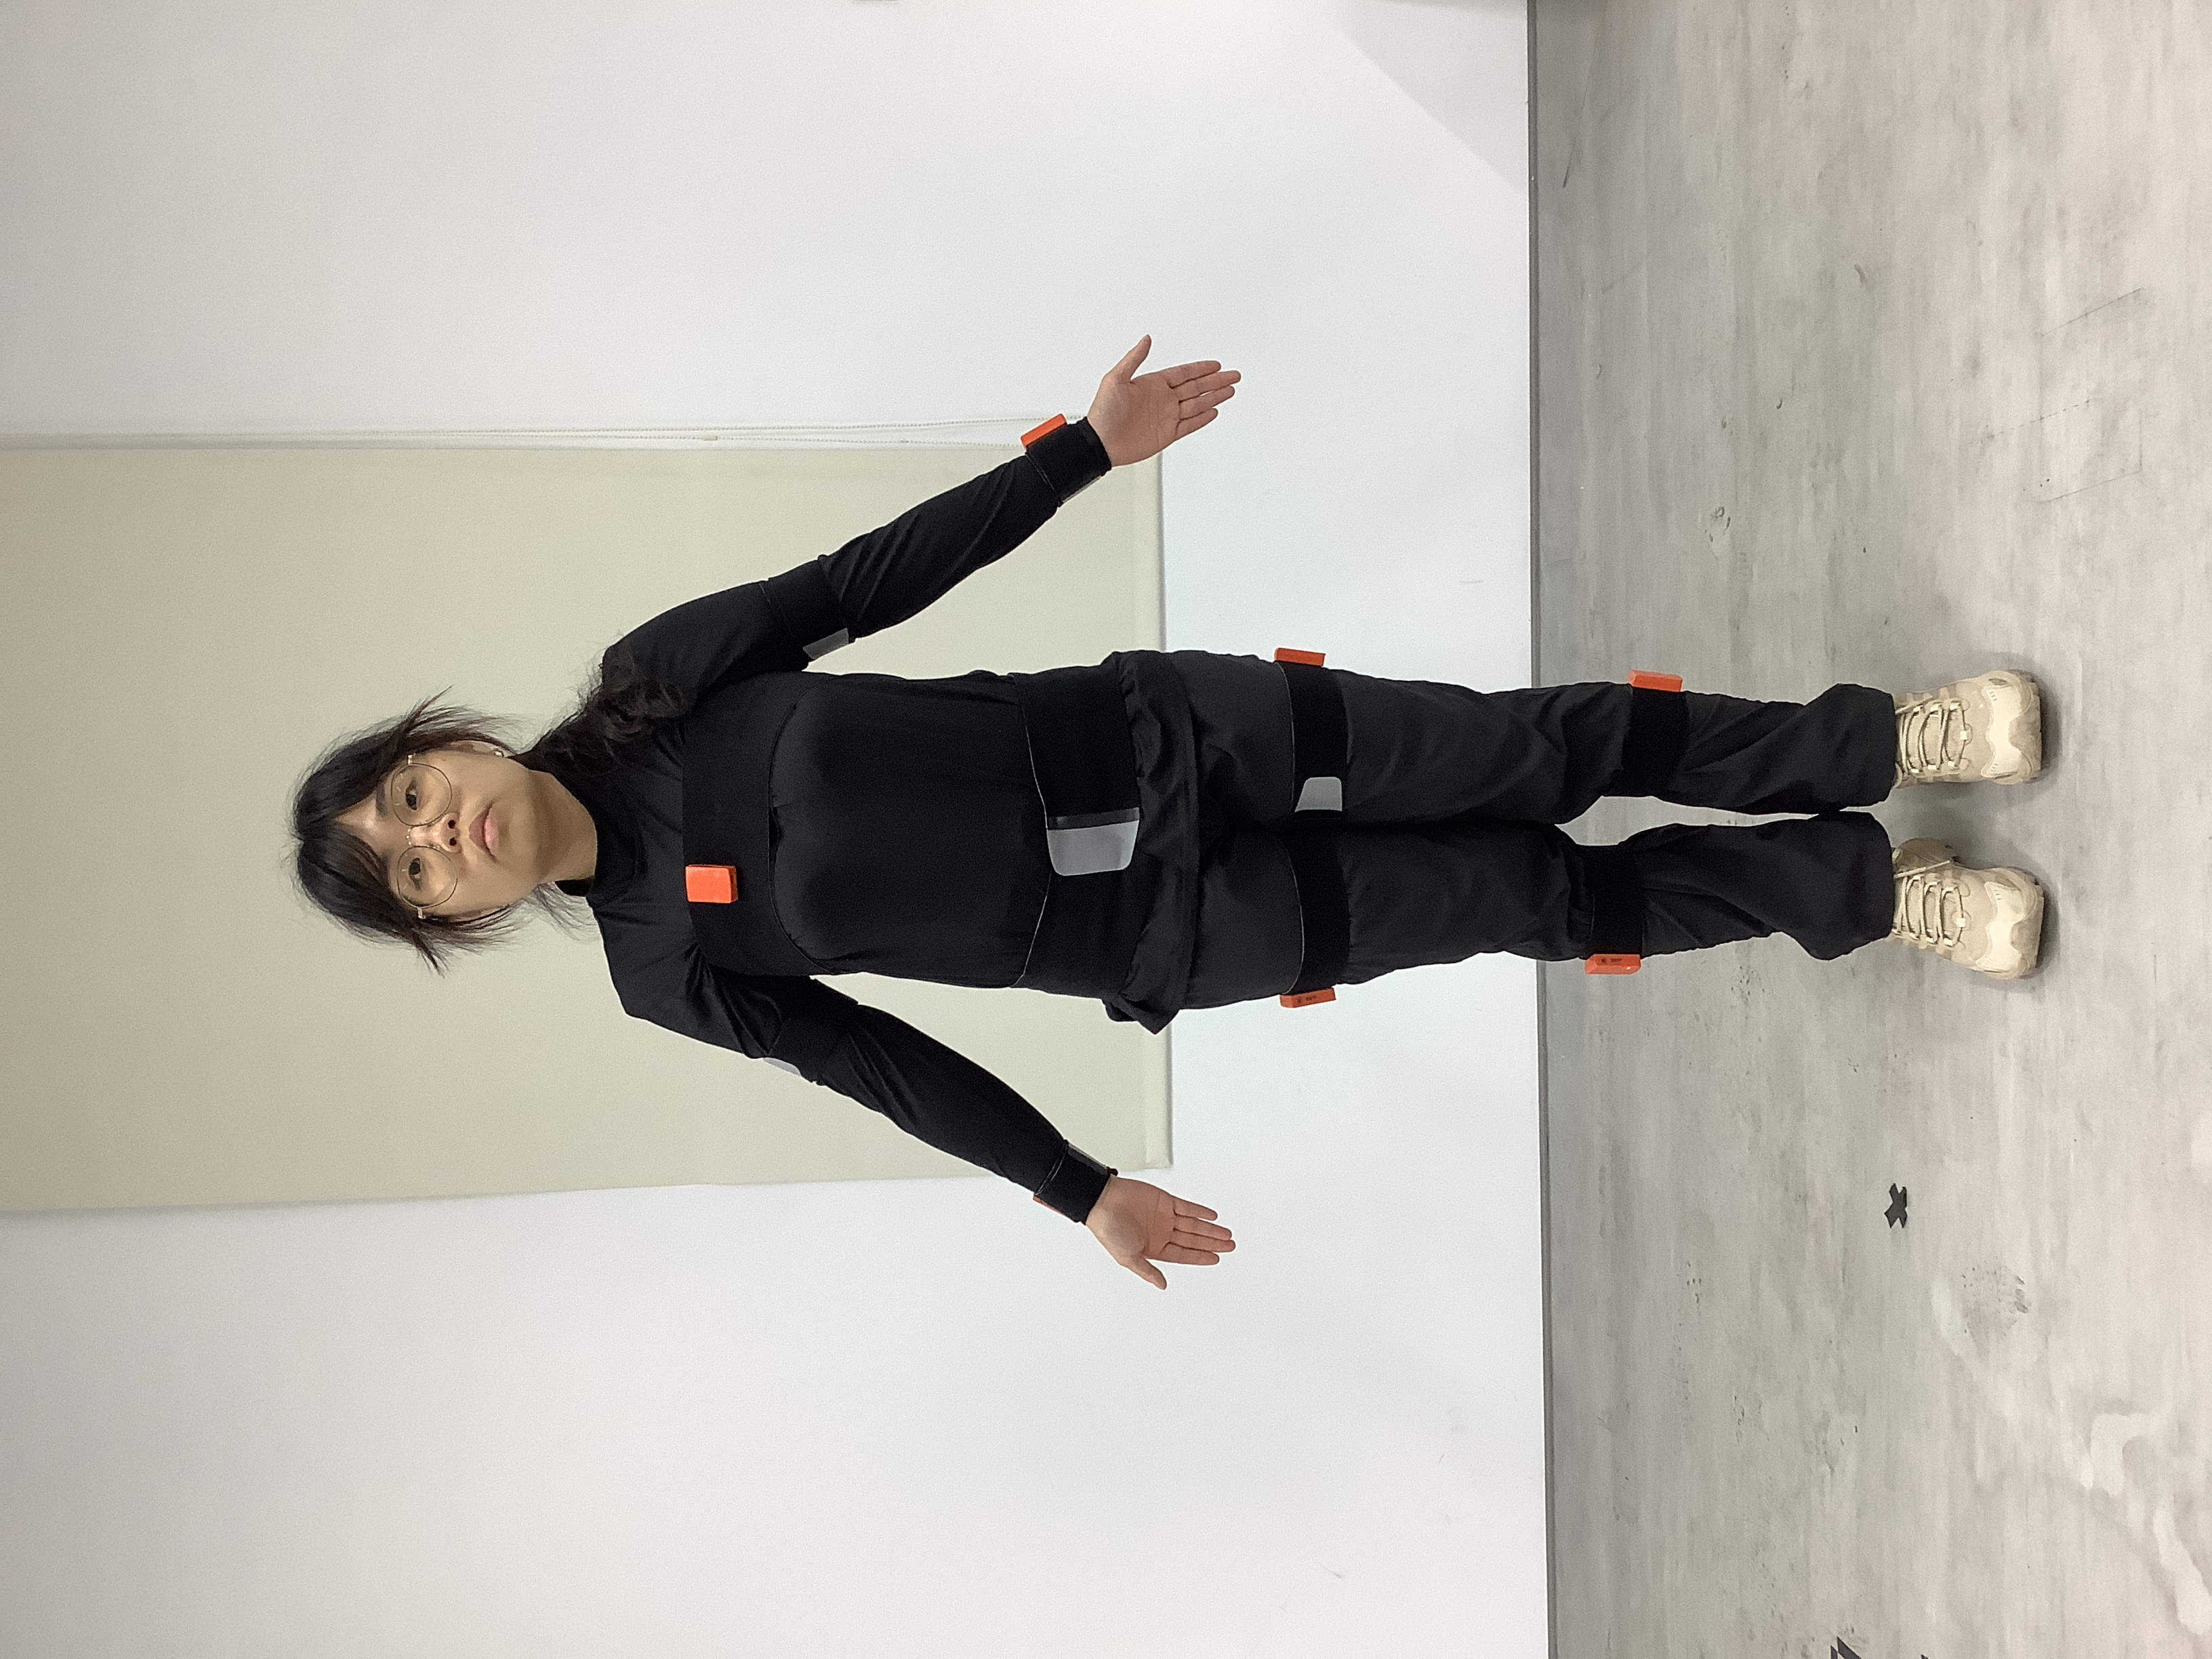
\includegraphics[width=\linewidth, angle=-90]{figure/ch3_fig_frontimu.JPG}
     \caption*{(a)}
   \end{minipage}%
   \begin{minipage}{.25\textwidth}
      \centering
      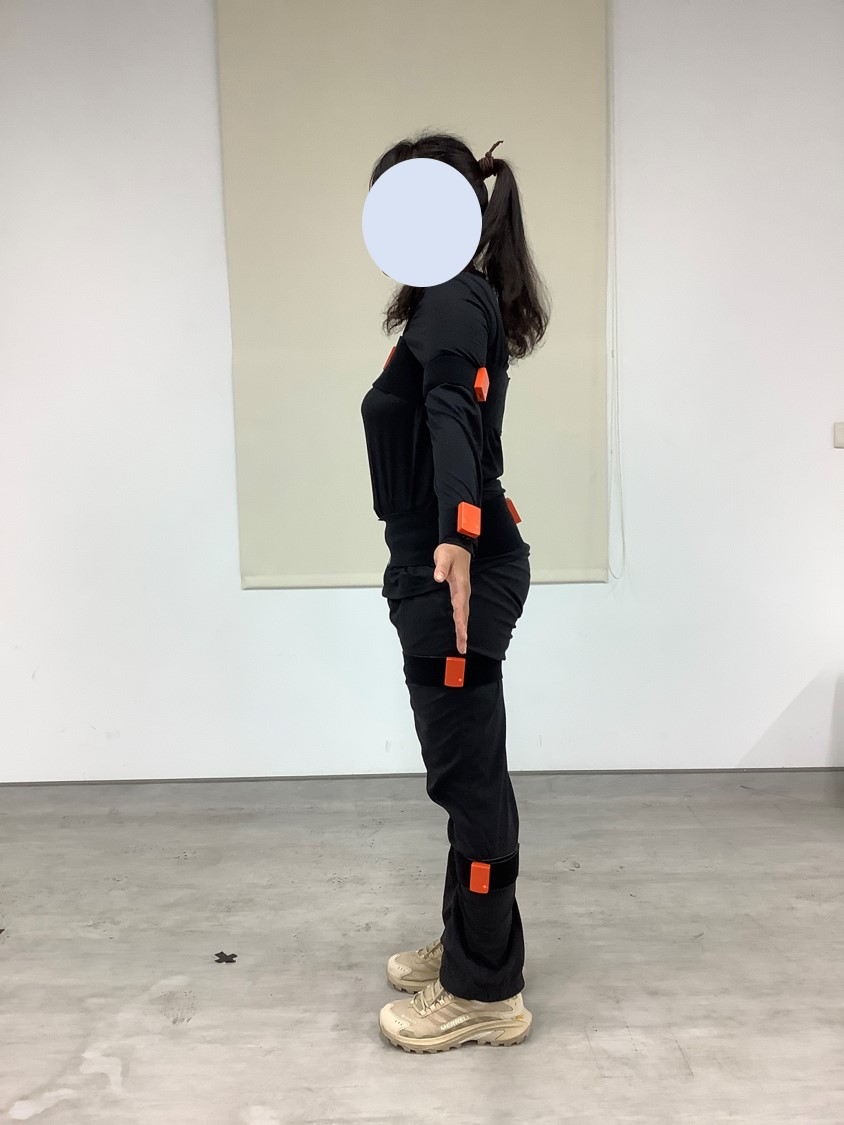
\includegraphics[width=\linewidth, angle=-90]{figure/ch3_fig_leftimu.JPG}
      \caption*{(b)}
   \end{minipage}%
   \begin{minipage}{.25\textwidth}
      \centering
      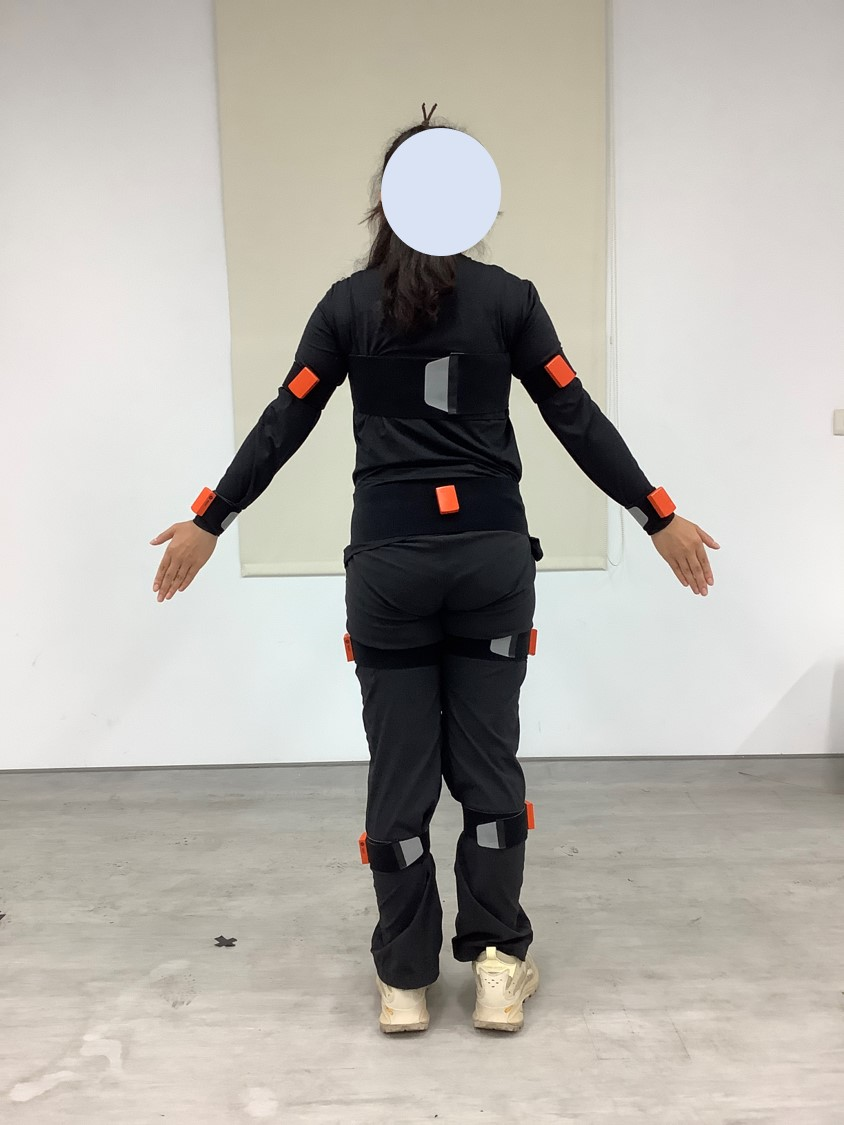
\includegraphics[width=\linewidth, angle=-90]{figure/ch3_fig_backimu.JPG}
      \caption*{(c)}
   \end{minipage}%
   \begin{minipage}{.25\textwidth}
     \centering
     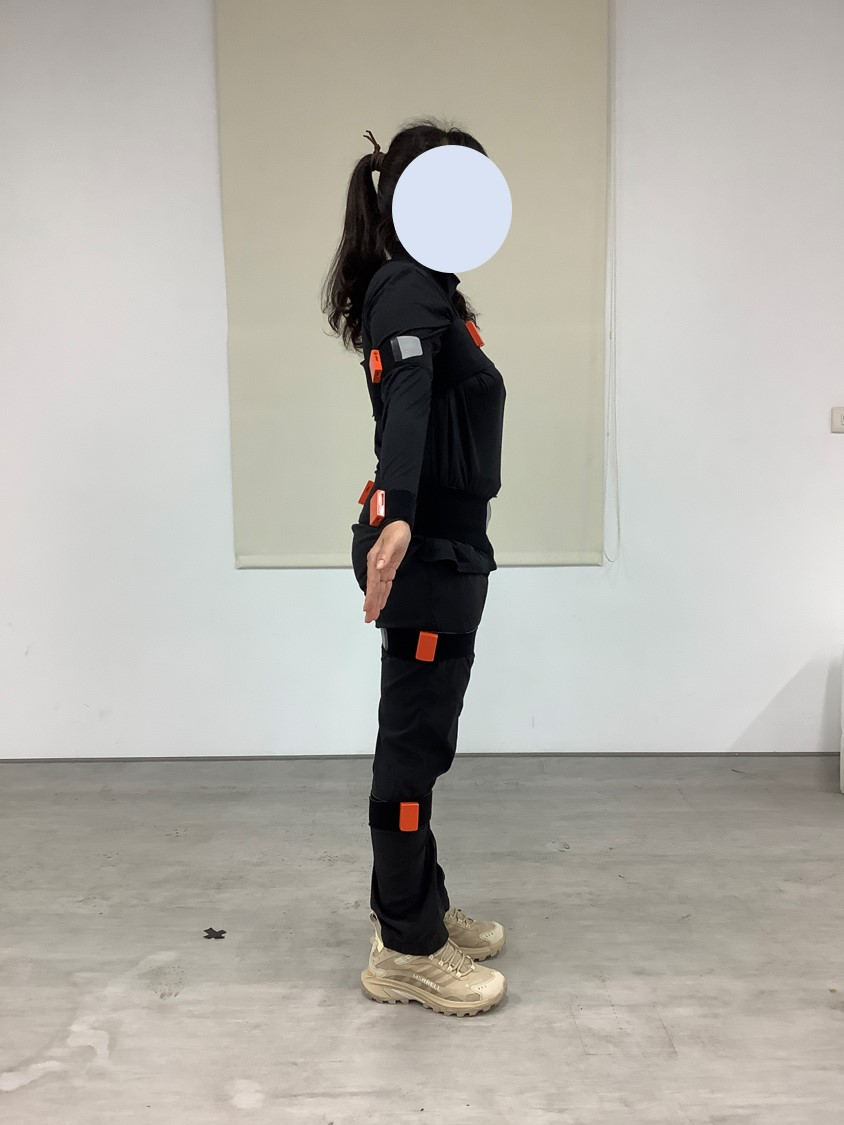
\includegraphics[width=\linewidth, angle=-90]{figure/ch3_fig_rightimu.JPG}
     \caption*{(d)}
   \end{minipage}
   \caption[IMU 於人體黏貼位置及方向 (a)前視(b)左視(c)後視(d)右視]{IMU 於人體黏貼位置及方向 (a)前視(b)左視(c)後視(d)右視}
   \label{ch3_fig_humanimu}
\end{figure}

\begin{figure}[!ht]
   \centering
   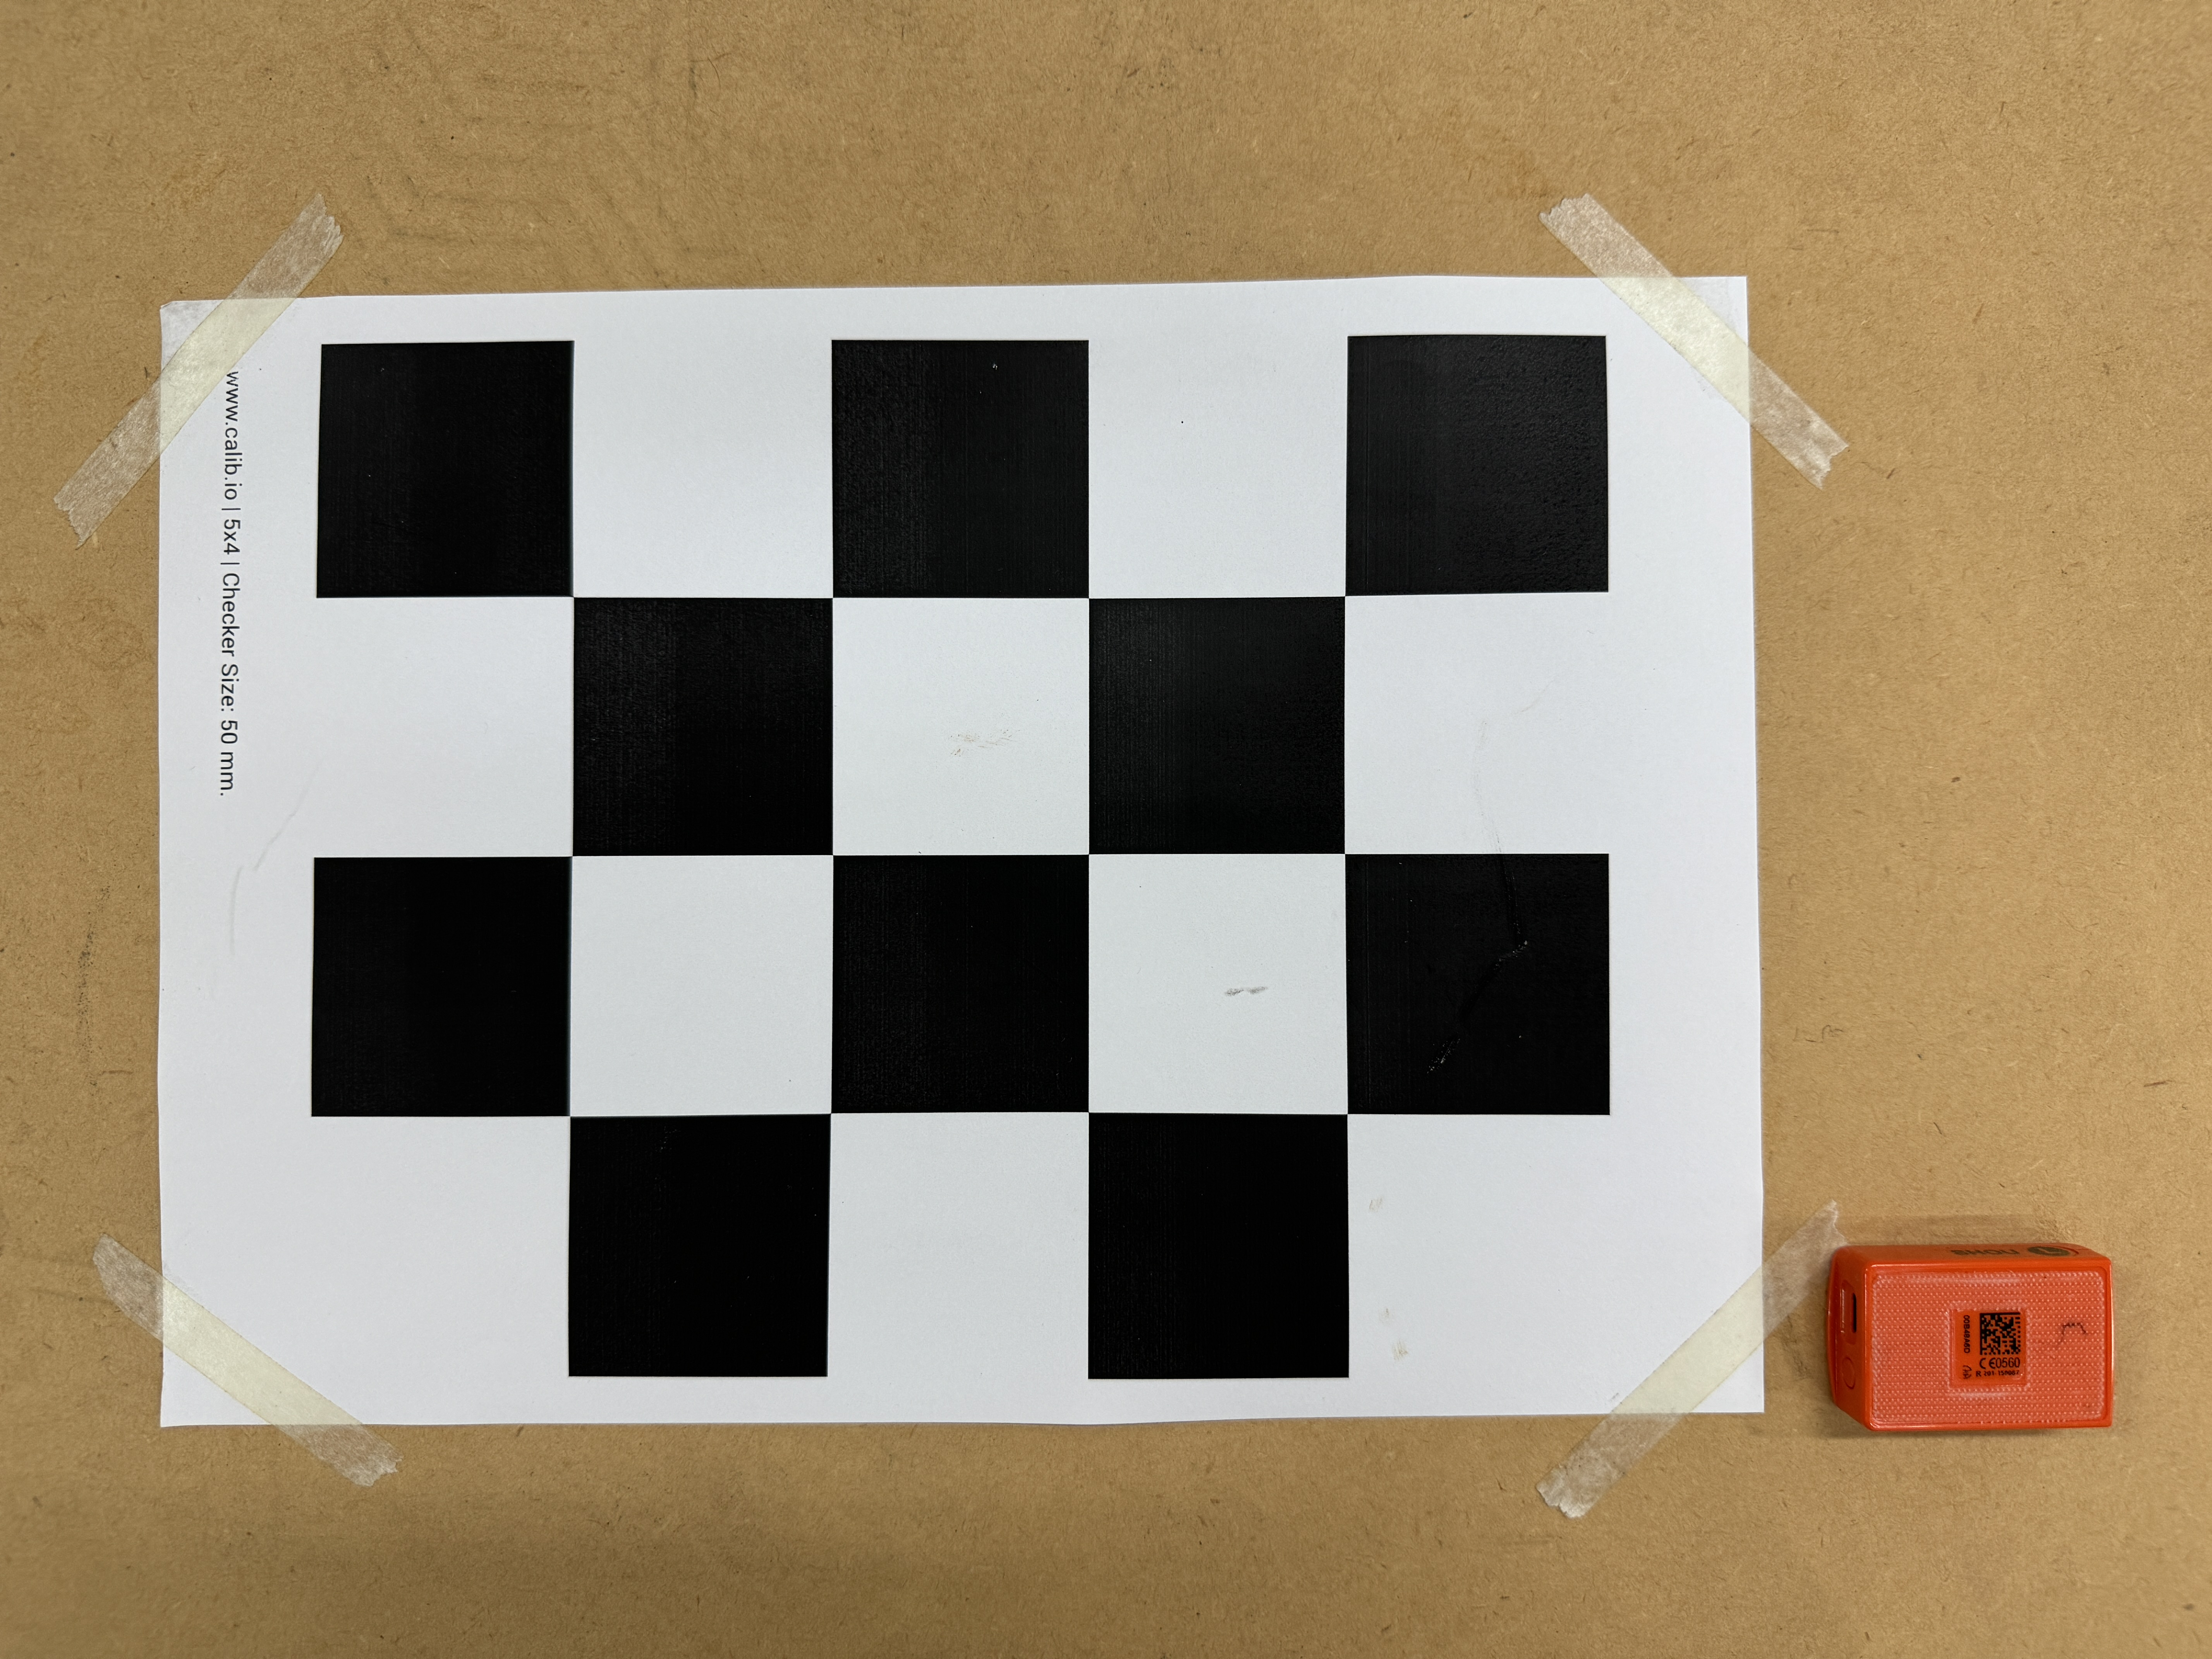
\includegraphics[width=8cm]{figure/ch3_fig_cbimu.JPG}
    \caption[IMU 於棋盤格校正板黏貼位置及方向]{IMU 於棋盤格校正板黏貼位置及方向}
    \label{ch3_fig_cbimu}
\end{figure}

\subsection{實驗環境}
% 實驗環境介紹
使用室內和室外環境,分開介紹

\subsubsection{室內實驗環境及尺寸}
% 室內實驗環境介紹
% 這邊可以放一張室內實驗環境的照片
所有房間尺寸、活動範圍尺寸、相機位置和高度

\subsubsection{室外實驗環境及尺寸}
% 室外實驗環境介紹
% 這邊可以放一張室外實驗環境的照片
所有房間尺寸、活動範圍尺寸、相機位置和高度

\subsection{實驗動作}
% 實驗動作介紹
現在還不確定要不要把每個動作的量測目的都寫出來,畢竟結果也不好

% ------------------------- 3.2 ------------------------- %
\section{資料前處理}
% 資料前處理介紹
利用章節~\ref{ch3_exp_setting} 介紹的系統蒐集完實驗資料後,接下來將進行資料前處理,以利後續進行感測器融合。
資料前處理分為人體立體骨架建立、獲取骨盆中點位置、時間對齊、空間對齊四個部分,將於本章節進行討論。

\subsection{人體立體骨架建立}\label{ch3_skeleton_method}
% 人體立體骨架建立介紹
% 伸縮沒有寫到,要怎麼加進去?
% TODO:覺得可以把我為甚麼選擇用 OpenPose 不用 mediapipe 寫在這邊
在文獻~\cite{zhang2020fusing} 中,作者使用 Vicon 系統所提供的立體骨架資料,
並以其為基礎,進行 IMU 計算;但是在非實驗室的環境中無法使用 Vicon 進行量測,進而取得立體骨架資料。
因此本研究透過 Pose2Sim~\cite{Pagnon_2021_Robustness}~\cite{Pagnon_2022_Accuracy}~\cite{Pagnon_2022_JOSS}提出之方法,
使用影像辨識技術,辨識每一視角中人體的關節點在影像中的位置,並利用相機校正技術建立出每一關節在空間中的位置,以此方式建立人體立體骨架。

章節~\ref{ch4_skeleton_exp} 將會利用 TotalCapture Dataset~\cite{Trumble:BMVC:2017}提供的影像資料,進行影像辨識與三角測量計算,
並將結果與 TotalCapture Dataset 提供之 Vicon 立體骨架資料比對,以驗證此方法的可行性。

\subsubsection{建立方法}
% 影像辨識
% 這邊好像跟第四章的4.1.1有點重複,如果這邊和4.1都要留的話可能就要把下一節的結果與驗證搬到4.1那邊
% 這邊就只要簡單介紹一下方法就好,然後這邊可以應該可以把為何要選 OpenPose 不選 mediapipe 也寫上去
% 只是這樣的話就要想一下4.1.2的實驗執行要怎麼寫(不然如果真的想不到可能就要刪掉實驗執行這塊,畢竟也只是 run 而已),
% 4.1.1的應該可以寫用了哪些數據
% 考慮要不要寫為何選擇使用 OpenPose 不選 mediapipe,要寫的話可以寫在這一段的開頭
本方法流程如圖~\ref{ch3_fig_skeleton_flow} 所示。
以 T pose 的姿勢拍攝影片後,進入後續軟體端處理流程。
首先,使用 OpenPose~\cite{8765346}~\cite{wei2016cpm}~\cite{simon2017hand}~\cite{cao2017realtime}
影像辨識技術辨識每一視角人體關節點在影像中的位置(使用 BODY-25B model),辨識結果如圖~\ref{ch3_fig_OpenPose_result} 所示,
其可辨識出左右肩膀、左右手肘、左右手腕、左右骨盆、左右膝蓋、左右腳踝等關節位置,如圖~\ref{ch3_fig_OpenPose} 所示;
接著,利用棋盤格方法之相機校正技術計算出各個相機的內部參數及外部參數;
再來,利用方才相機校正之結果,經由三角測量計算建立出關節在空間中的位置,並使用距離公式計算每一關節之間的距離;
最後,基於 TotalCapture Dataset 提供之 vicon 立體骨架,利用計算出的距離進行立體骨架伸縮,
得到與受試者四肢、身高相似之立體骨架,如圖~\ref{ch3_fig_my_skeleton}。

\begin{figure}[!ht]
   \centering
   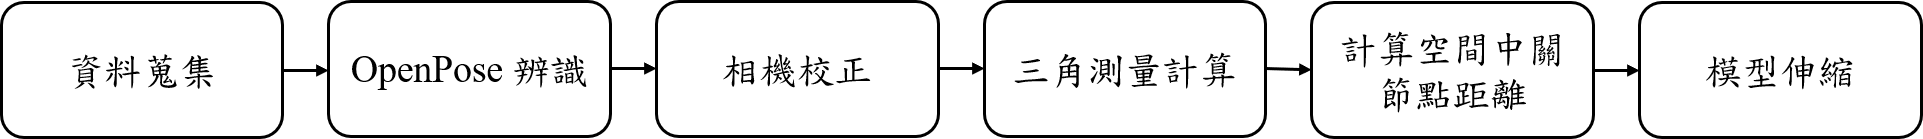
\includegraphics[width=\linewidth]{figure/ch3_fig_skeleton_flow.png}
    \caption[立體骨架建立流程圖]{立體骨架建立流程圖}
    \label{ch3_fig_skeleton_flow}
\end{figure}

\begin{figure}[!ht]
   \centering
   \includegraphics[width=8cm]{figure/ch3_fig_OpenPose_result.png}
   \caption[OpenPose 辨識結果]{OpenPose 辨識結果}
   \label{ch3_fig_OpenPose_result}
\end{figure}

\begin{figure}[!ht]
   \centering
   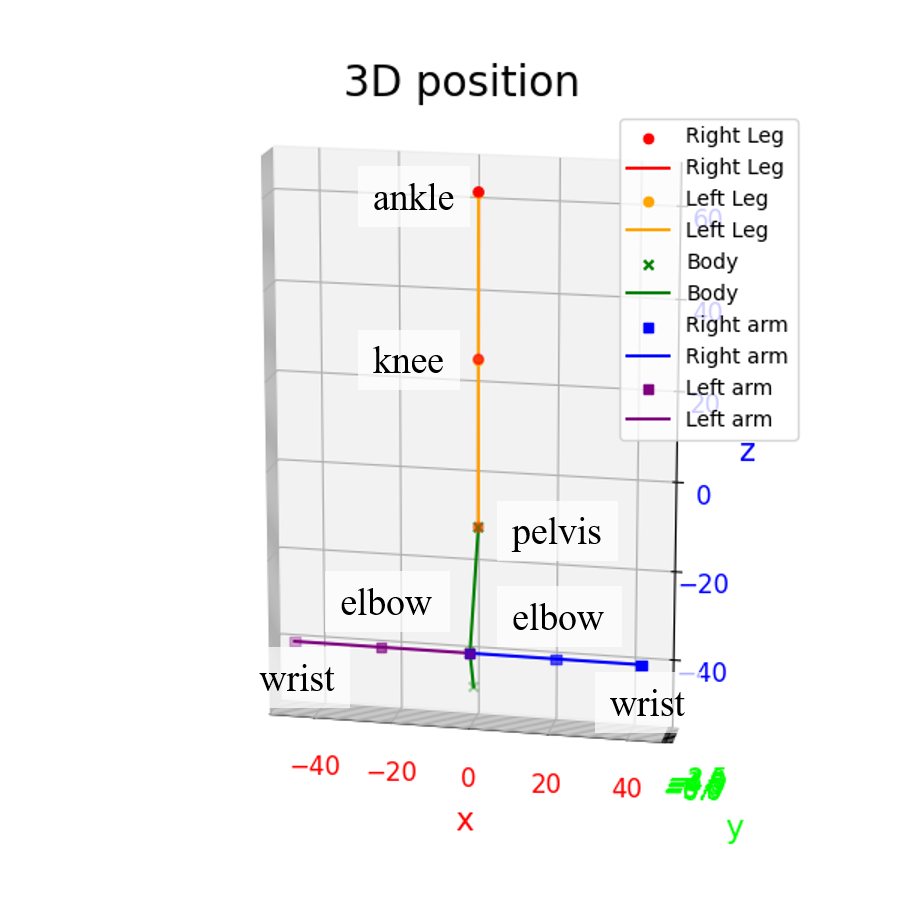
\includegraphics[width=8cm]{figure/ch3_fig_my_skeleton.png}
   \caption[立體骨架建立結果]{立體骨架建立結果}
   \label{ch3_fig_my_skeleton}
\end{figure}

\subsection{計算骨盆在影像中的像素位置}
% 軟體介紹;OpenPose
% OpenPose 為一款
% 由  Ginés Hidalgo, Zhe Cao, Tomas Simon, Shih-En Wei, Yaadhav Raaj, Hanbyul Joo, and Yaser Sheikh 等人開發的開源軟體,
% 為第一個在單個圖像上可以同時偵測人體關節、手部關節、面部表情和足部關鍵點(總共 135 個關鍵點)的實時多人偵測系統,
% 其可於 Windows、MacOS、Ubuntu 等作業系統上執行,並支援 Python、C++ 等程式語言,
% 輸入資源包括圖片、影像、網路攝影機等,
% 並可輸出原始影像加關鍵點顯示的疊圖 (PNG,JPG,AVI,...),
% 或是輸出純文字檔案 (JSON,XML,YAML...),其中紀錄關鍵點相對於輸入圖像的像素座標位置及 0~1 的分數。
本研究使用 OpenPose 作為影像辨識工具,搭配其提供之 BODY\_25B 模型進行影像辨識,
辨識出每一幀照片中 25 個人體關鍵點在圖像中的像素位置,可辨識出的關鍵點如圖~\ref{ch3_fig_OpenPose} 所示,
並進一步計算左骨盆及右骨盆的中點在圖像中的像素位置,以此計算結果作為該張影像的中點進行畫面裁切,減低後續感測器融合的計算量。

\begin{figure}[!ht]
   \centering
   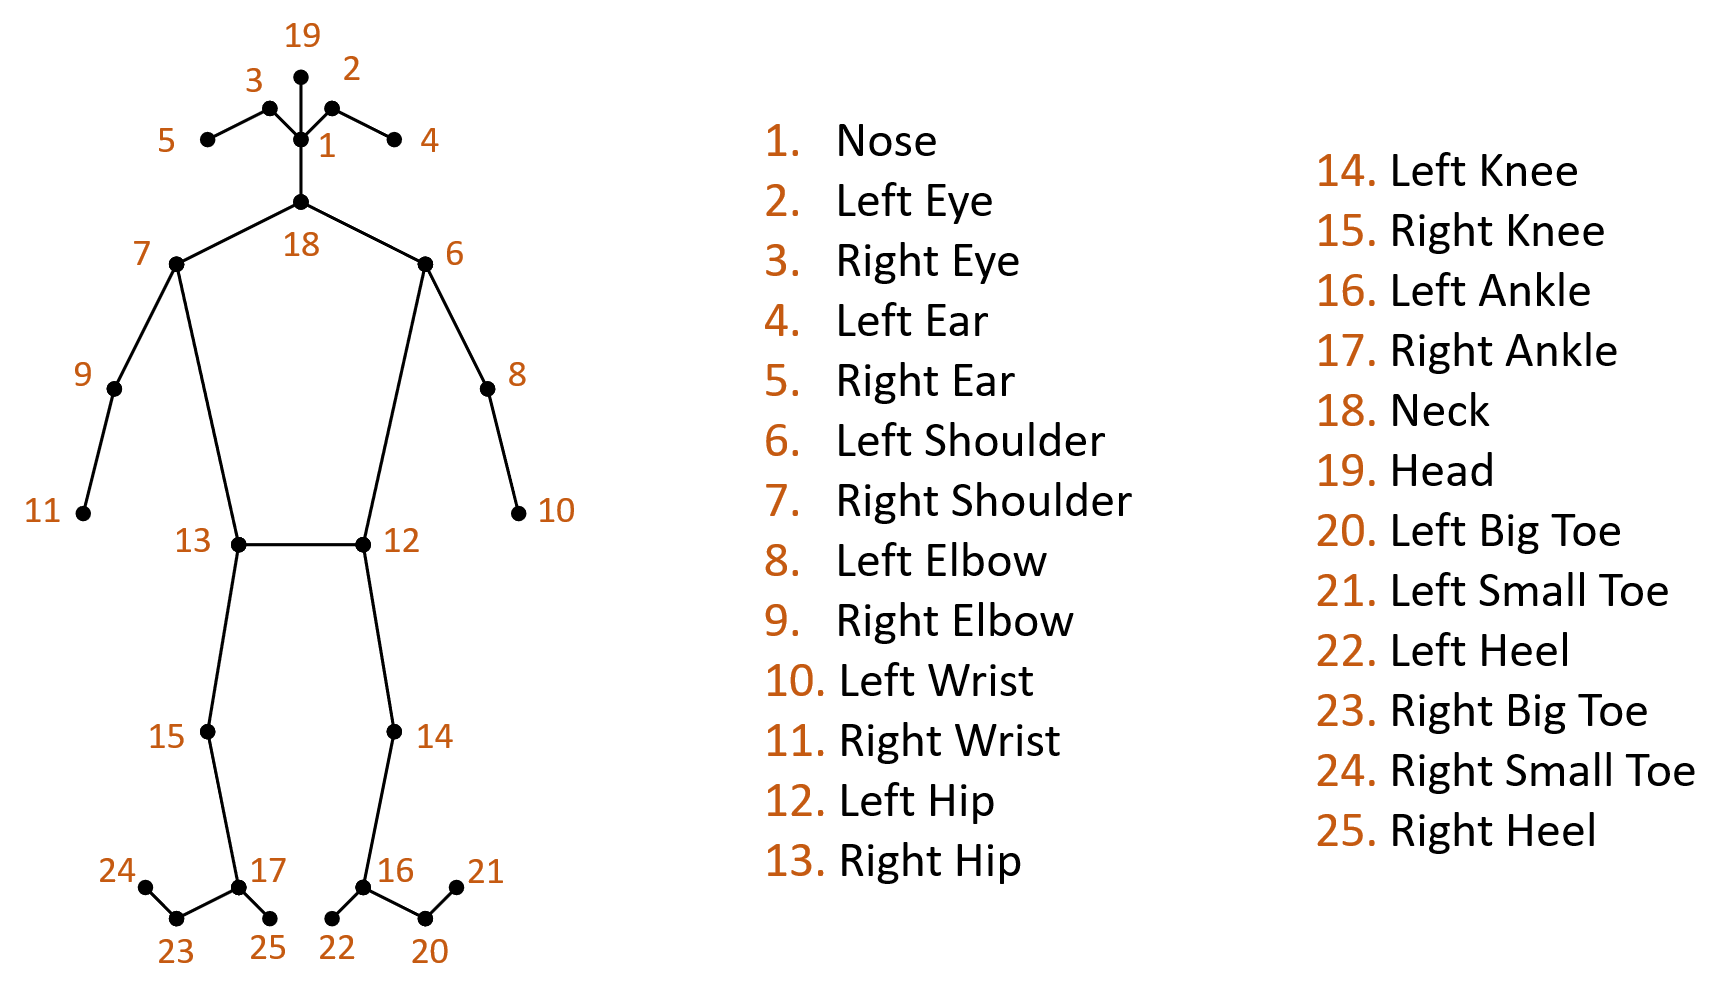
\includegraphics[width=\linewidth]{figure/ch3_fig_OpenPose.png}
    \caption[OpenPose 關節點對應位置]{OpenPose 關節點對應位置}
    \label{ch3_fig_OpenPose}
\end{figure}

\subsection{時間對齊}
% 時間軸對齊介紹
本研究參考的方法進行時間對齊,在實驗動作開始及結束時,受試者皆需進行拍手動作,
動作流程為:兩手打直張開呈現 T 姿勢維持 1~2 秒,然後迅速合攏雙手並拍手,最後維持合掌姿勢 1~2 秒。
透過拍手動作,可在影像資料的音軌中找到明顯地拍手聲音,
並在 IMU 資料中找到快速拍手動作的時間點,因為迅速合攏手掌的拍手動作會產生明顯的加速度變化,
以此時間點作為時間對齊的基準點,將影像資料及 IMU 資料進行時間對齊,以確保兩者之間的時間軸一致。
在對齊並剪輯影像資料及 IMU 資料時有一點需要注意,
裁切 IMU 資料時,需將拍手動作前後一個時間差的資料保留,以確保拍手動作的加速度變化完整呈現,
因此進行影像剪輯時,需將合掌姿勢前後一個時間差的影像資料保留,以確保拍手動作的完整呈現,且可與 IMU 資料對齊。
% TODO:等第二章時間對齊的部分寫完記得來 cite clappping 那一篇

\subsection{空間對齊}
% 座標系轉換介紹
在人體量測領域中,每一量測方法都有其固有且常用之座標系,
因此在進行感測器融合時,必須將各感測器之座標系轉換至同一座標系,以方便後續感測器融合計算。
本研究共涉及六種座標系,可分為影像系統及 IMU 感測器系統兩大部分,兩部分的共同座標系為全域座標系 (g)。
影像系統涉及三種座標系,分別為圖像座標系 (cb)、相機座標系 (cam) 及全域座標系 (g);
IMU 感測系統則涉及四種座標系,分別為骨骼座標系 (b)、感測器座標系 (s)、IMU local 座標系 (i)、全域座標系 (g)。
各座標系的定義及轉換關係將於以下進行介紹。

\subsubsection{座標系定義}
% 各座標系定義介紹
圖像座標系為二維座標系,以圖像左上角為原點,x 軸沿圖像右側為延伸為正,y 軸沿圖像下側延伸為正,如圖~\ref{ch3_fig_frame} (a) 所示;
相機座標系以相機的光心為原點,z 軸與光軸重和,指向相機前方為正, x 軸指向相機右方為正, y 軸指向相機下方為正,如圖~\ref{ch3_fig_frame} (b) 所示;
骨骼座標系以 TotalCapture Dataset 提供之 Vicon 立體骨架所在之座標系為基礎,如圖~\ref{ch3_fig_frame} (c) 所示,
其以人體骨盆中心為原點, +x、+y、+z 方向分別為向右 (red)、向後 (green)、向下 (blue);
感測器座標系,以感測器本身為原點,
於 Xsens 系統中,定義其 x 軸為長邊延伸方向,y 軸為短邊延伸方向,z 軸則沿最大平面法向,
如圖~\ref{ch3_fig_frame} (d) 所示;
IMU local 座標系以感測器所在地為原點,y 軸沿子午線指向正北為正,z 軸指向天頂為正,x 軸與 yz 平面垂直,指向正東為正;
全域座標系以固定的全球基準點為原點 (例如地球中心),x 軸以磁北極為參考方向,z 軸參考方向與 IMU local 座標系 z 軸相同,指向天頂為正,
y 軸則以右手定則決定,通常指向西方為正。
座標系間的關係及旋轉矩陣將於下一段進行介紹。

\begin{figure}[!ht]
   \centering
   \begin{minipage}{.5\textwidth}
      \centering
      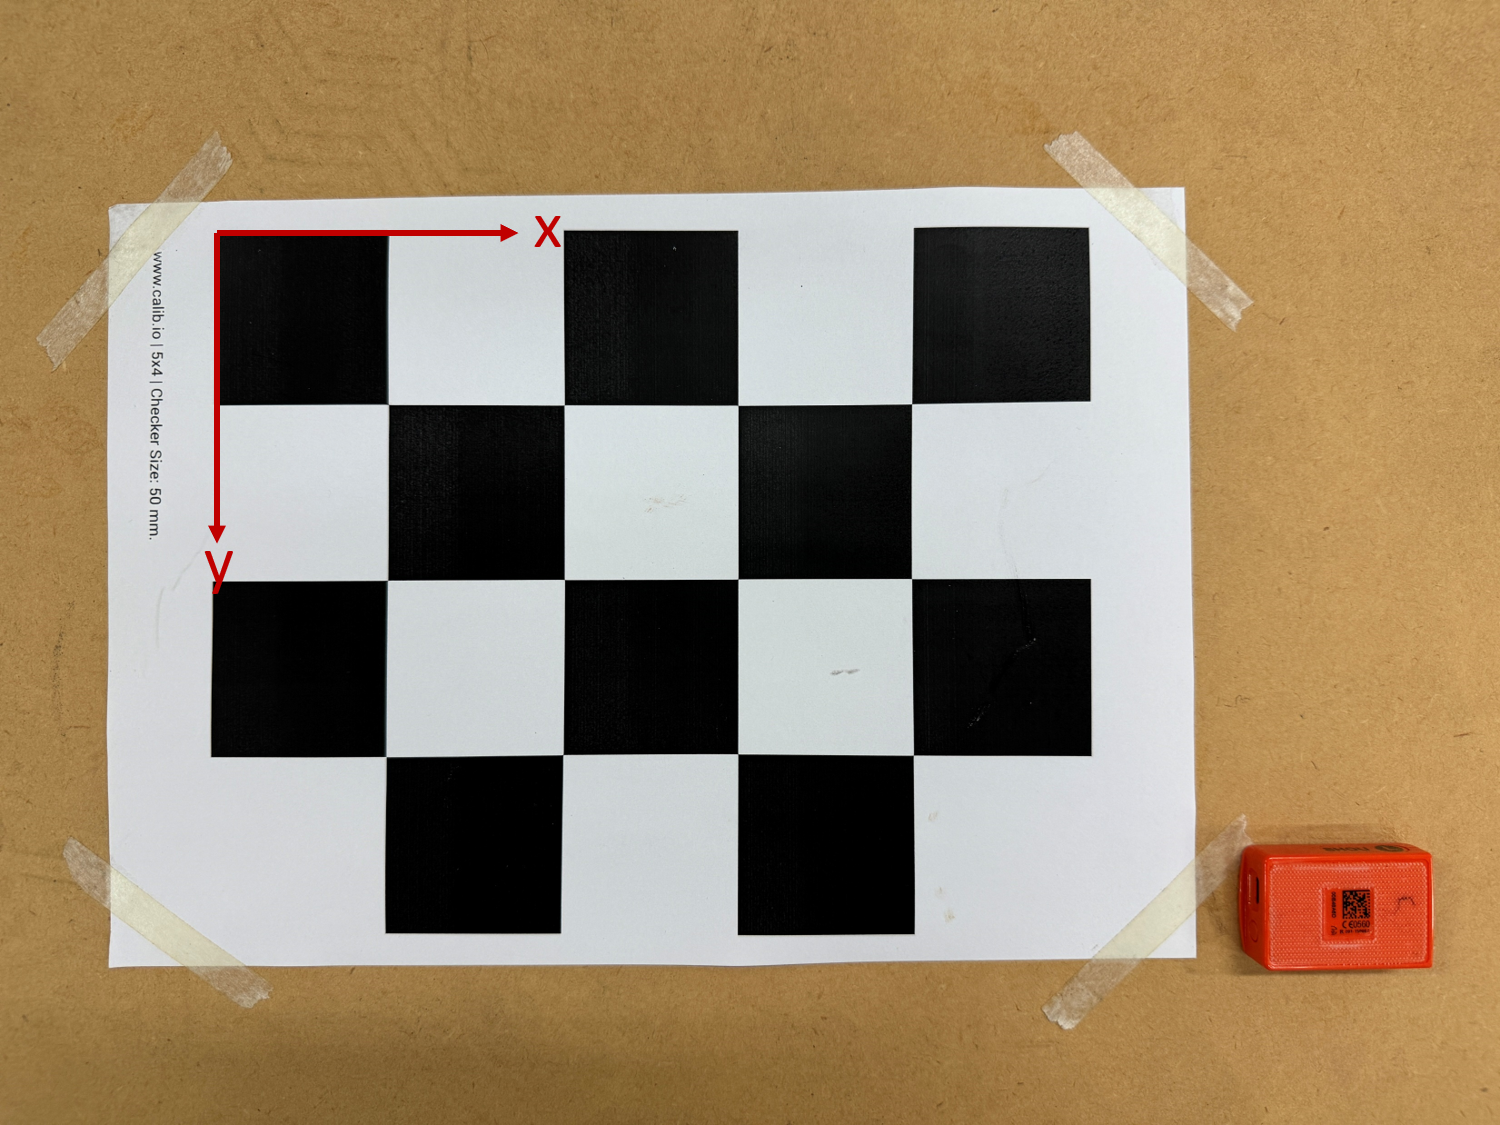
\includegraphics[width=\linewidth]{figure/ch3_fig_cbframe.png}
      \caption*{(a)}
   \end{minipage}%
   \vspace{5mm}%
   \begin{minipage}{.5\textwidth}
      \centering
      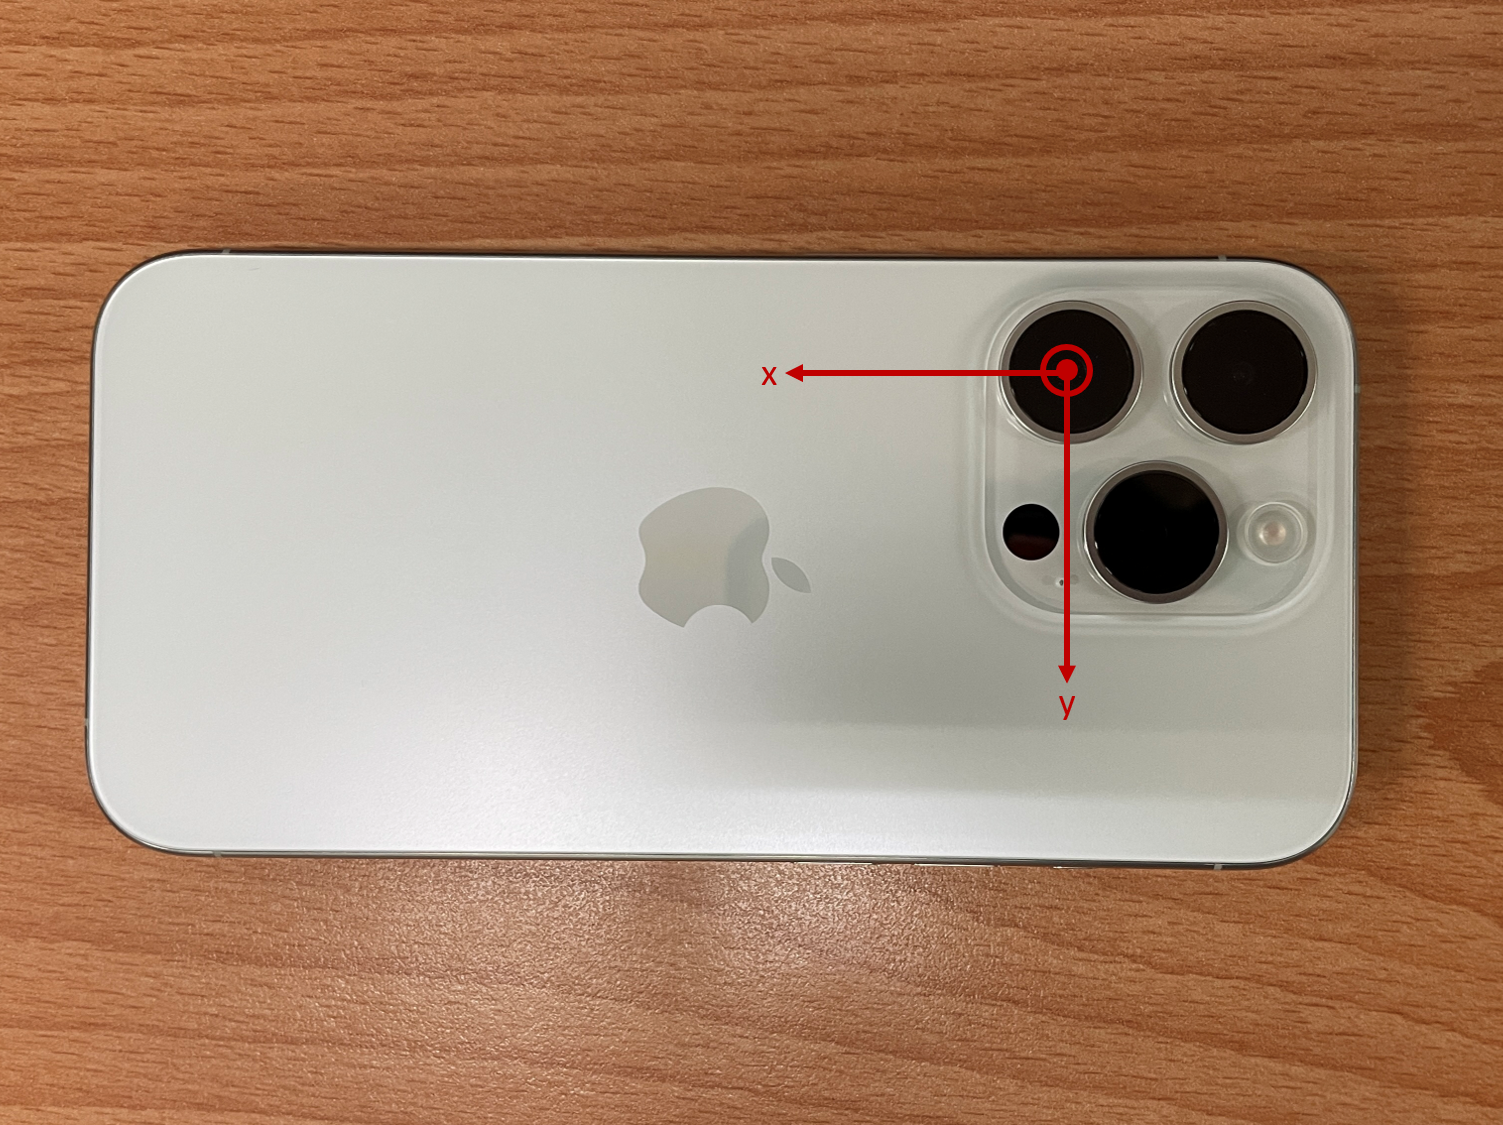
\includegraphics[width=\linewidth]{figure/ch3_fig_camframe.png}
      \caption*{(b)}
   \end{minipage}
   \begin{minipage}{.5\textwidth}
     \centering
     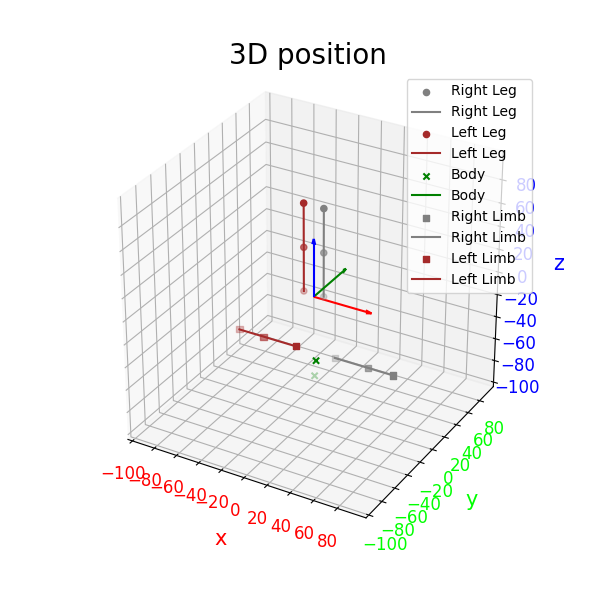
\includegraphics[width=\linewidth]{figure/ch3_fig_skeleton_frame.png}
     \caption*{(c)}
   \end{minipage}%
   \begin{minipage}{.5\textwidth}
     \centering
     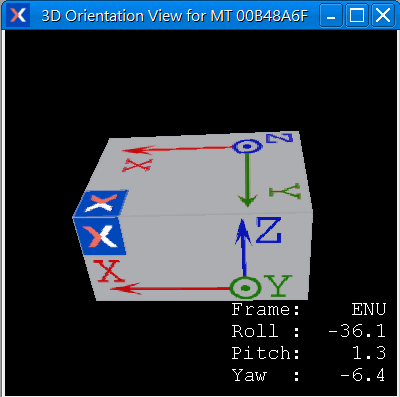
\includegraphics[width=\linewidth]{figure/ch3_fig_imu_frame.png}
     \caption*{(d)}
   \end{minipage}
   \caption[座標系定義 (a)影像座標系 (b)相機座標系 (c)骨骼座標系 (d)感測器座標系]{座標系定義 (a)影像座標系 (b)相機座標系 (c)骨骼座標系 (d)感測器座標系}
   \label{ch3_fig_frame}
\end{figure}

\subsubsection{各座標系間的關係}
% 各座標系間的關係介紹
在影像系統座標系定義與轉換的部分,本研究使用關係式~\ref{ch3_equ_image_rotation_matrix},
將在空間中的位置點由以全域座標系為表示方式轉換至以相機座標系為表示方式。

\begin{equation}
   R^{cam}_{g} = R^{cam}_{cb}(R^{g}_{cb})^{-1}
   \label{ch3_equ_image_rotation_matrix}
\end{equation}

其中,$R^{cam}_g$ 為將空間中的位置點由全域座標系轉換至相機座標系之旋轉矩陣,
即圖~\ref{ch3_fig_coordinate_trans} 中,從綠色座標系轉換至紫色座標系之旋轉矩陣,
通過將 $R^{cam}_g$ 乘以全域座標系中的骨骼朝向,將以全域座標系表示之朝向轉換為以相機座標系表示的骨骼朝向;
$(R^{g}_{cb})^{-1}$ 為全域座標系轉換至圖像座標系之旋轉矩陣,
即圖~\ref{ch3_fig_coordinate_trans} 中,從綠色座標系轉換至粉色座標系之旋轉矩陣,
通過將 $R^{cam}_g$ 乘以全域座標系中的骨骼朝向,將以全域座標系表示之朝向轉換為以圖像座標系表示的骨骼朝向;
$R^{cam}_{cb}$ 為圖像座標系轉換至相機座標系之旋轉矩陣,
即圖~\ref{ch3_fig_coordinate_trans} 中,從粉色座標系轉換至紫色座標系之旋轉矩陣,
通過將 $R^{cam}_{cb}$ 乘以圖像座標系中的骨骼朝向,將以圖像座標系表示之朝向轉換為以相機座標系表示的骨骼朝向。

在 IMU 感測器系統座標系定義與轉換的部分,
本研究參考文獻~\cite{malleson2017real}所提出之關係式~\ref{ch3_equ_imu_rotation_matrix},並進行修正以更有助於理解,
將每一關節點由以骨骼座標系為表示方式轉換至以全域座標系為表示方式。

\begin{equation}
   R^g_b=R^g_iR^i_s(R^b_s)^{-1}
   \label{ch3_equ_imu_rotation_matrix}
\end{equation}

其中,$R^g_b$ 為將 IMU 所附著的骨骼朝向由骨骼座標系轉換至全域座標系之旋轉矩陣,
即圖~\ref{ch3_fig_coordinate_trans} 中,從黑色座標系轉換至綠色座標系之旋轉矩陣,
通過將 $R^g_b$ 乘以骨骼座標系中的骨骼朝向,將以骨骼座標系表示之朝向轉換為以全域座標系表示的骨骼朝向;
$(R^b_s)^{-1}$ 為骨骼座標系轉換至感測器座標系之旋轉矩陣,
即圖~\ref{ch3_fig_coordinate_trans} 中,從黑色座標系轉換至紅色座標系之旋轉矩陣,
通過將 $(R^b_s)^{-1}$ 乘以骨骼座標系中的骨骼朝向,將以骨骼座標系表示之骨骼朝向轉換為以感測器座標系表示的骨骼朝向;
$R^i_s$ 為感測器座標系轉換至 IMU local 座標系之旋轉矩陣,
即圖~\ref{ch3_fig_coordinate_trans} 中,從紅色座標系轉換至藍色座標系之旋轉矩陣,
通過將 $R^i_s$ 乘以感測器座標系中的骨骼朝向,將以感測器座標系表示之骨骼朝向轉換為以 IMU local 座標系表示的骨骼朝向;
$R^g_i$ 為 IMU local 座標系轉換至全域座標系之旋轉矩陣,
即圖~\ref{ch3_fig_coordinate_trans} 中,從藍色座標系轉換至綠色座標系之旋轉矩陣,
通過將 $R^g_i$ 乘以 IMU local 座標系中的骨骼朝向,將以 IMU loccal 座標系表示之骨骼朝向轉換為以全域座標系表示的骨骼朝向。
上述所提即之每一旋轉矩陣的量測與計算方式將於後續進行介紹。

\begin{figure}[!ht]
   \centering
   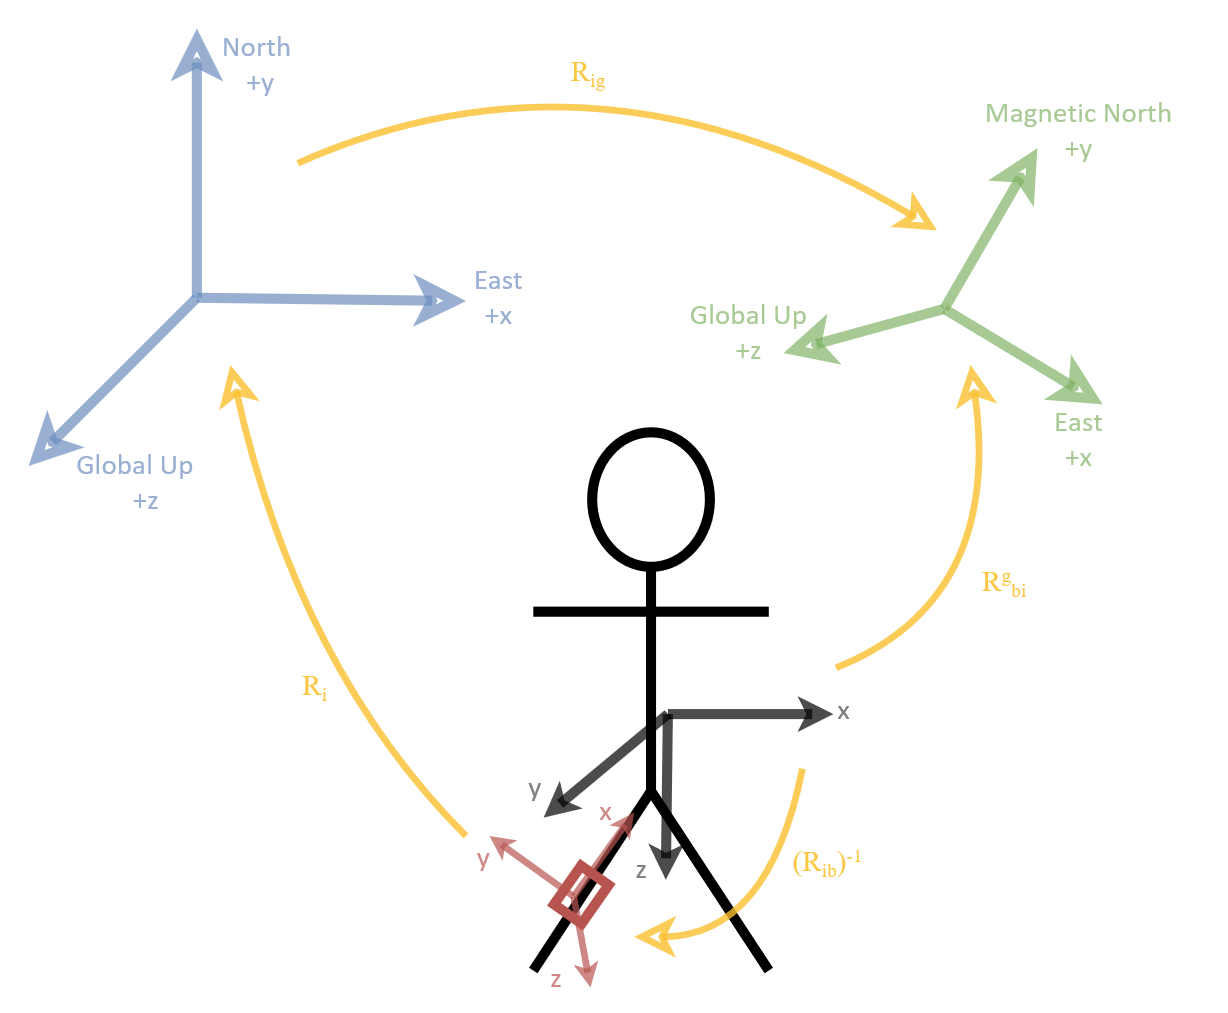
\includegraphics[width=\textwidth]{figure/ch3_fig_coordinate_trans.png}
    \caption[各座標系間的關係]{各座標系間的關係}
    \label{ch3_fig_coordinate_trans}
\end{figure}

\subsubsection{圖像座標 - 全域座標旋轉矩陣,$R^{g}_{cb}$}
%圖像座標 - 全域座標旋轉矩陣
圖像座標 - 全域座標旋轉矩陣 ($R^{g}_{cb}$) 為計算受試者手上棋盤格校正板與全域座標系間關係之旋轉矩陣,
其可將圖像座標系轉換至全域座標系,
將座標系統一轉換到全域座標系,以方便後續進行感測器融合計算。
圖像座標 - 全域座標旋轉矩陣計算方式如方程式~\ref{ch3_equ_cb2g_rotation_matrix} ,
本研究將棋盤格校正板安裝上 IMU,並將棋盤格校正板的 x、y 座標方向與 IMU 的 x、y 對齊,
經過對齊後,IMU 的朝向可直接視為棋盤格校正板的朝向,因此 $R^{i}_{cb} = R^{i}_{s}$,
經由 IMU 量得的 IMU - IMU local 旋轉四元數即可視為棋盤格校正板 - IMU local 的旋轉四元數,
再將整體座標系對 y 軸旋轉 $90^{\circ}$ ,對 x 軸旋轉 $180^{\circ}$ ,即可得到圖像座標 - 全域座標旋轉矩陣。

\begin{equation}
   R^{g}_{cb} = R_{x}(\theta_{x})R{y}(\theta_{y})R^{i}_{cb} = R_{x}(\theta_{x})R{y}(\theta_{y})R^{i}_{s}
   \label{ch3_equ_cb2g_rotation_matrix}
\end{equation}

\subsubsection{圖像座標 - 相機座標旋轉矩陣,$R^{cam}_{cb}$}
% 圖像座標 - 相機座標旋轉矩陣
圖像座標 - 相機座標旋轉矩陣 ($R^{cam}_{cb}$) 為計算受試者手上棋盤格校正板與相機間關係之旋轉矩陣,
其可將圖像座標系轉換至相機座標系,
本研究之計算方式為使用一 5x4,方格寬度為 50 (mm) 的棋盤格校正板,
並使用 Pose2SimPose2Sim~\cite{Pagnon_2021_Robustness}~\cite{Pagnon_2022_Accuracy}~\cite{Pagnon_2022_JOSS} 提供的校正工具進行外部參數及內部參數計算,
透過相機校正所得之外部參數即為棋盤格校正板與相機間的旋轉及平移關係。

\subsubsection{感測器座標 - 骨骼座標旋轉矩陣,$R^b_s$}
% IMU - 骨骼座標轉換矩陣計算介紹
% 解釋表示方法是以哪個座標系去看哪個座標系,然後解釋計算方法
使用 IMU 進行肢體朝向量測時,由於 IMU 黏貼於肢體上的方向及位置可能會和骨骼定義之方向及位置有所偏差,
因此需使用感測器座標 - 骨骼座標旋轉矩陣($R^b_s$),將位於感測器座標系的量測數值轉換為以骨骼座標系表示的骨骼朝向。
感測器座標 - 骨骼座標旋轉矩陣計算方式如方程式~\ref{ch3_equ_b2s_rotation_matrix},
假設受試者在最初始開始實驗時,設定一個與 IMU local 座標系對齊的座標系統,且受試者的姿勢為 T 姿勢,
因此此時 IMU 到其附著肢段的旋轉矩陣與 IMU 到 IMU local 的旋轉矩陣相同,即 $R^{b}_{s}(t_0) = R^{i}_{s}(t_0)$,
因此,在 $t_0$ 時刻量得的 IMU - IMU local 旋轉四元數即可視為感測器座標 - 骨骼座標旋轉四元數,
而由於在章節~\ref{ch3_skeleton_method} 中建立的骨架座標與 IMU 附著於骨骼定義的座標系相差 $180^{\circ}$,
因此,再將整體座標系對 x 軸旋轉 $180^{\circ}$ ,即可得最終感測器座標 - 骨骼座標旋轉矩陣。 

\begin{equation}
   R^{b}_{s} = R_{x}(\theta_{x})R^{b}_{s}(t_0) = R_{x}(\theta_{x})R^{i}_{s}(t_0)
   \label{ch3_equ_b2s_rotation_matrix}
\end{equation}

% 此矩陣可經由 OpenSim~\cite{delp2007opensim}處理並進一步計算而得,其取得及計算方式如下。
% 首先,量測結束之 IMU 資料將透過 OpenSim 軟體進行處理,\sout{使用基礎骨骼模型...},計算每一 IMU 相對其對應骨骼之相對位置及角度,
% 處理結果可經由 OpenSim 軟體可視化,如圖~\ref{ch3_fig_imu_ori} 所示。
% 此項數據紀錄於 OpenSim 輸出之 .osim 檔案的 <BodySet> 元素中,<BodySet> 以骨骼為單位,
% 其中包含之 <components> 則記錄一附著於該骨骼上之 IMU 的相對位置及角度,
% <translation> 代表該 IMU 的原點相對於其附著之骨骼原點的平移,
% <orientation> 則代表該 IMU 的座標軸相對於其附著之骨骼坐標軸的旋轉。
% 因此若將 <translation> 數值更改為零,則可看到 IMU 原點與骨骼原點重合,如圖~\ref{ch3_fig_imu_tra},
% 而若將 <orientation> 數值更改為零,則可看到 IMU 坐標軸與骨骼坐標軸平行,如圖~\ref{ch3_fig_imu_rot}。
% 因此,從 .osim 檔案取得每一 IMU 相對於骨骼之相對位置及角度後,即可計算出感測器座標 - 骨骼座標四元數。
% \begin{figure}[!ht]
%    \centering
%    \begin{minipage}{.3\textwidth}
%      \centering
%      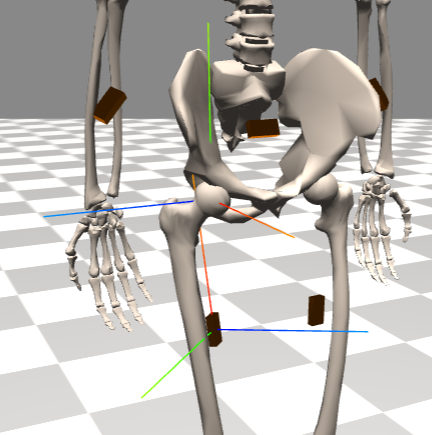
\includegraphics[width=.8\linewidth, height=.8\linewidth]{figure/ch3_fig_imu_ori.png}
%      \caption[OpenSim 計算結果]{OpenSim 計算結果}
%      \label{ch3_fig_imu_ori}
%    \end{minipage}%
%    \begin{minipage}{.3\textwidth}
%      \centering
%      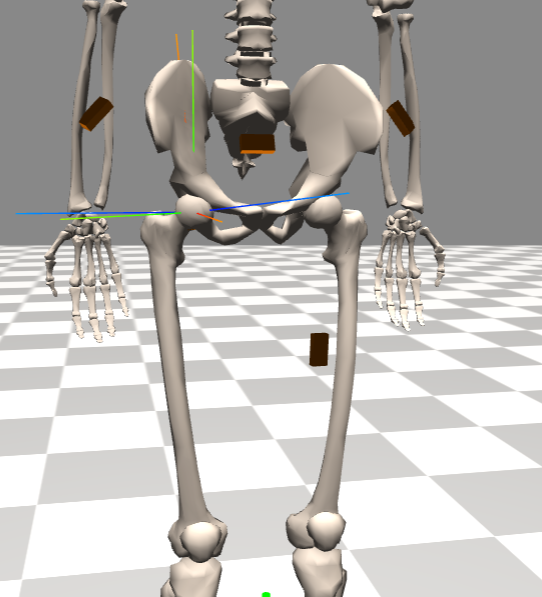
\includegraphics[width=.8\linewidth, height=.8\linewidth]{figure/ch3_fig_imu_tra.png}
%      \caption[IMU 平移為零]{IMU 平移為零}
%      \label{ch3_fig_imu_tra}
%    \end{minipage}%
%    \begin{minipage}{.3\textwidth}
%       \centering
%       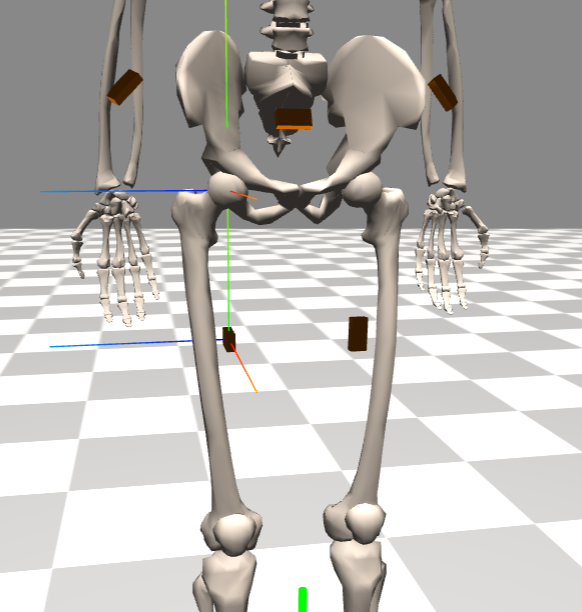
\includegraphics[width=.8\linewidth, height=.8\linewidth]{figure/ch3_fig_imu_rot.png}
%       \caption[IMU 旋轉為零]{IMU 旋轉為零}
%       \label{ch3_fig_imu_rot}
%     \end{minipage}
% \end{figure}

\subsubsection{感測器座標 - IMU local 旋轉矩陣,$R^i_s$}
經過上一步 $(R^b_s)^{-1}$ 的轉換,已將骨骼朝向轉換為以附著其上的 IMU 感測器座標系為表示方式,
接著,需要進一步將各自表示的感測器座標系轉換至統一以東北天 (East - North - Up, ENU) 為定義的 IMU local 座標系。
感測器座標 - IMU local 旋轉矩陣 ($R^i_s$) 為 IMU 的量測朝向,可直接經由 Xsens 系統所提供軟體 (MT manager) 輸出四元數取得。
在 MT manager 中讀入量測時所記錄的 .mtb 檔案,
% TODO:...模型為基礎
並於 file>export 中的輸出選項勾選 quaternion 後輸出,
每一 .txt 檔案中的 q0、q1、q2、q3 即為將朝向旋轉成以 IMU local 座標系為表示方式的旋轉四元數,分別代表四元數的 w、x、y、z,
將四元數轉換為旋轉矩陣即可得感測器座標 - IMU local 旋轉矩陣。

\subsubsection{IMU local - 全域座標旋轉矩陣,$R^g_i$}
% IMU - 全域座標轉換矩陣計算介紹
% 解釋表示方法是以哪個座標系去看哪個座標系,然後解釋計算方法
經過上一步 $R^i_s$ 的轉換,已將骨骼朝向轉換為以統一的 IMU local 感測器座標系為表示方式,
接著,為方便後續與影像辨識而得的位置資訊進行融合,需要進一步將骨骼朝向轉換至位置資訊所在之座標系。
假設所有 IMU 間的 IMU local - 全域座標旋轉矩陣 $R^g_i$ 皆一致,且與天頂及磁北極對齊,
再將整體座標系相對 x 軸旋轉 $-90^{\circ}$,即可得 IMU local - 全域座標旋轉矩陣。
% 包含兩個階段的旋轉,
% 第一階段先將於 IMU local 座標系的骨骼朝向轉換至以全域座標系表示,與天頂及磁北極對齊,
% 第二階段將於全域座標系的骨骼朝向轉換至位置資訊所在之座標系,該座標系相對全域座標系的 x 軸旋轉 $-90^{\circ}$。
% 在第一階段中,IMU local - 全域座標的轉換與磁偏角 ($\delta$) 有關,
% 將 IMU local 座標系繞 z 軸旋轉 $\delta$ 即可轉換至全域座標系。
% 第二階段再將全域座標系繞 x 軸旋轉 $-90^{\circ}$,轉換至位置資訊所在之座標系。

% ------------------------- 3.3 ------------------------- %
\section{感測器融合方法}
% 感測器融合方法介紹
% 這邊如果篇幅過大也可以另立成3.3,cameraset 就改成 3.4
IMU image pytorch

% ------------------------- 3.4 ------------------------- %
\section{探討減少相機數量的可行性}
% 探討減少相機數量的可行性及其擺放位置介紹,可是擺放位置的結論還沒有可以很好的呈現方式,所以暫時先不要有這方面的結論和討論
% TODO:可以從增加實驗架設方便性方面作為開頭著手
TotalCapture Dataset~\cite{Trumble:BMVC:2017}提供 8 台相機與 13 個 IMU 的量測資料,
而在文獻~\cite{zhang2020fusing}中,作者使用到 4 台相機及 8 個 IMU 的資料;
另外在 TotalCapture Dataset 發表的文獻~\cite{Trumble:BMVC:2017}中則有提及嘗試減少相機的硬體數量,準確度隨著相機數量的減少而下降,
因此本章節嘗試以減少相機數量\sout{並選擇相機擺放位置}進行感測器融合計算的方式,
探討減少相機使用數量對於動作捕捉的影響,\sout{並嘗試探討相機擺放位置的選擇}。

\subsection{實驗方法}
% 實驗方法介紹
% 目前的相機用量及擺放位置敘述,要 cite totalcapture 和 data fusion
TotalCapture Dataset 實驗環境為一個 4x6 (m) 的方形空間,每一面牆面上方架設兩台相機,
四面牆共計八台相機,每台相機距離地面高度皆為 2.5 (m),擺放位置以上視的視角呈現,如圖~\ref{ch3_fig_cameraset_totalcap} 所示。
本次實驗將分成七類情況進行,第一類情況為從八台相機中任選一台相機進行感測器融合計算,
並將得到的姿勢估計結果與 TotalCapture Dataset 提供的 Vicon 位置資料進行比對,計算平均每關節誤差 (mean per joint position error, MPJPE),
第二類為任選兩台相機進行姿勢估計,以此方式遞增至第七類,任選七台相機進行姿勢估計,每一類情況皆會產生一組 MPJPE。

\begin{figure}[!ht]
   \centering
   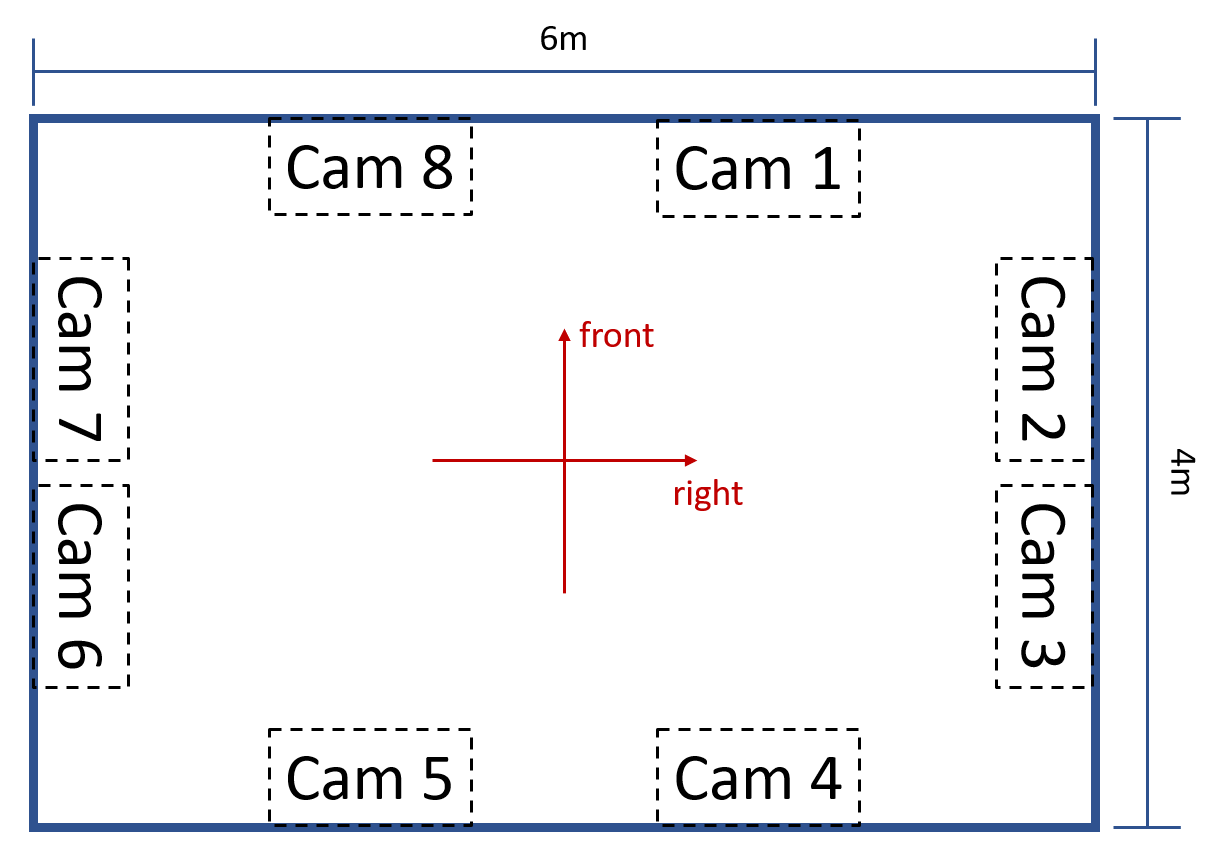
\includegraphics[width=8cm]{figure/ch3_fig_cameraset_totalcap.png}
    \caption[相機擺放位置]{相機擺放位置}
    \label{ch3_fig_cameraset_totalcap}
\end{figure}

\subsection{實驗結果}
% 實驗結果
經過上述七類情況之實驗後,得到的 MPJPE 結果如以下所示。

\subsubsection{一台相機}
將圖~\ref{ch3_fig_cameraset_totalcap} 中的相機任選一台進行估計,共計有 8 種估計結果,每一結果皆可計算出 MPJPE,
MPJPE 計算結果如表~\ref{ch3_cameraset_1cam} 所示,可以發現無論選擇哪一個位置的相機,其估計誤差皆超過 500 (mm)。
標準差為 87.6016 (mm),平均值為 599.8855 (mm)。
% 因此本研究認為只使用一台相機進行估計是不可行的,至少需使用兩台相機進行量測。
\begin{table}[!ht]
   \caption[一台相機組合與其估計結果誤差]{一台相機組合與其估計結果誤差}
   \centering
   \label{ch3_cameraset_1cam}
   \setlength{\tabcolsep}{3pt}
   \renewcommand\arraystretch{1.5}
   \resizebox{\textwidth}{!}{
   \begin{tabular}{
   >{\columncolor[HTML]{E7E6E6}}c |c|
   >{\columncolor[HTML]{E7E6E6}}c |c|
   >{\columncolor[HTML]{E7E6E6}}c |c|
   >{\columncolor[HTML]{E7E6E6}}c |c}
      相機配置 & MPJPE & 相機配置 & MPJPE & 相機配置 & MPJPE & 相機配置 & MPJPE \\
      \hline
      1	& 514.76 & 2 & 782.01 & 3 & 611.84 & 4 & 520.97 \\
      5	& 653.96 & 6 & 573.41 & 7 & 599.78 & 8 & 542.36 \\
   \end{tabular}}
\end{table}
\clearpage

\subsubsection{兩台相機}
將圖~\ref{ch3_fig_cameraset_totalcap} 中的相機任選兩台進行排列組合,共計有 28 種組合方式之估計結果,每一結果皆可計算出 MPJPE,
MPJPE 計算結果如表~\ref{ch3_cameraset_2cam} 所示,其中最佳組合方式為相機 18,其 MPJPE 為 46.9798 (mm);
而最差組合方式為相機 25,其 MPJPE 為 300.1637 (mm)。標準差為 61.7928 (mm),平均值為 109.8694 (mm)。
經由平均值可以發現兩台相機的姿勢估計表現相對一台相機的姿勢估計表現有大幅度的進步,進步幅度約為 500 (mm);
但是由標準差可知兩台相機的姿勢估計結果仍不穩定。
% 經由結果可以發現相機的擺放位置對估計結果影響甚鉅,若位置選擇得宜,估計結果將會相當準確,反之則會有較大的誤差。
\begin{table}[!ht]
   \caption[兩台相機組合與其估計結果誤差]{兩台相機組合與其估計結果誤差}
   \centering
   \label{ch3_cameraset_2cam}
   \setlength{\tabcolsep}{3pt}
   \renewcommand\arraystretch{1.5}
   \resizebox{\textwidth}{!}{
   \begin{tabular}{
   >{\columncolor[HTML]{E7E6E6}}c |c|
   >{\columncolor[HTML]{E7E6E6}}c |c|
   >{\columncolor[HTML]{E7E6E6}}c |c|
   >{\columncolor[HTML]{E7E6E6}}c |c}
      相機配置 & MPJPE & 相機配置 & MPJPE & 相機配置 & MPJPE & 相機配置 & MPJPE \\
      \hline
      12 & 194.4957 & 13 & 81.9440 & 14 & 47.4927 & 15 & 76.7795 \\
      16 & 66.8653 & 17 & 58.7619 & 18 & 46.9798 & & \\
      \hline
      23 & 227.5722 & 24 & 182.6378 & 25 & 300.1637 & 26 & 183.0773 \\
      27 & 181.6520 & 28 & 145.2458 & & & &\\
      \hline
      34 & 99.3426 & 35 & 109.4178 & 36 & 92.7550 & 37 & 97.7435 \\
      38 & 81.3640 & & & & & &\\
      \hline
      45 & 87.4750 & 46 & 66.8800 & 47 & 67.4949 & 48 & 52.3318 \\
      \hline
      56 & 126.3387 & 57 & 95.1469 & 58 & 64.6374 & &\\
      \hline
      67 & 100.7632 & 68 & 63.7904 & & & &\\
      \hline
      78 & 77.1948 & & & & & &\\
   \end{tabular}}
\end{table}
\clearpage

\subsubsection{三台相機}
將圖~\ref{ch3_fig_cameraset_totalcap} 中的相機任選三台進行排列組合,共計有 56 種組合方式之估計結果,每一結果皆可計算出 MPJPE,
MPJPE 計算結果如表~\ref{ch3_cameraset_3cam} 所示,其中最佳組合方式為相機 137,其 MPJPE 為 27.1579 (mm);
而最差組合方式為相機 257,其 MPJPE 為 82.8158 (mm)。標準差為 13.8423 (mm),平均值為 42.9001 (mm)。
經由平均值可以發現:相較兩台相機的姿勢估計結果,三台相機的姿勢估計結果準確性仍有明顯提升,進步幅度約為 60 (mm);
由標準差可以知道三台相機的姿勢估計結果漸趨穩定。
% 但只要位置恰當,僅用三台相機也可以有四台相機的表現水準。
\begin{table}[!ht]
   \caption[三台相機組合與其估計結果誤差]{三台相機組合與其估計結果誤差}
   \centering
   \label{ch3_cameraset_3cam}
   \setlength{\tabcolsep}{3pt}
   \renewcommand\arraystretch{1.5}
   \resizebox{\textwidth}{!}{
   \begin{tabular}{
   >{\columncolor[HTML]{E7E6E6}}c |c|
   >{\columncolor[HTML]{E7E6E6}}c |c|
   >{\columncolor[HTML]{E7E6E6}}c |c|
   >{\columncolor[HTML]{E7E6E6}}c |c|
   >{\columncolor[HTML]{E7E6E6}}c |c}
      相機配置 & MPJPE & 相機配置 & MPJPE & 相機配置 & MPJPE & 相機配置 & MPJPE & 相機配置 & MPJPE \\
      \hline
      123 & 41.8538 & 124 & 43.2544 & 125 & 70.4747 & 126 & 41.7470 & 127 & 54.5721 \\
      128 & 46.7714 & & & & & & & & \\
      134 & 30.9862 & 135 & 29.0275 & 136 & 33.6116 & 137 & 27.1579 & 138 & 29.9961 \\
      145 & 34.4860 & 146 & 32.7227 & 147 & 29.9785 & 148 & 31.5573 & & \\
      156 & 38.3802 & 157 & 33.2107 & 158 & 33.4297 & & & & \\
      167 & 32.4098 & 168 & 33.4044 & 178 & 32.2636 & & & & \\
      \hline
      234 & 52.0193 & 235 & 76.4435 & 236 & 52.6657 & 237 & 65.5297 & 238 & 44.5936 \\
      245 & 76.6047 & 246 & 42.4841 & 247 & 54.8719 & 248 & 45.2496 & & \\
      256 & 74.8608 & 257 & 82.8158 & 258 & 62.4336 & & & & \\
      267 & 58.7578 & 268 & 39.2619 & 278 & 62.7102 & & & & \\
      \hline
      345 & 35.9928 & 346 & 42.7418 & 347 & 35.2381 & 348 & 33.5695 & & \\
      356 & 42.9933 & 357 & 35.1894 & 358 & 29.6995 & & & & \\
      367 & 40.0411 & 368 & 35.8360 & 378 & 34.9221 & & & & \\
      \hline
      456 & 40.0658 & 457 & 37.2030 & 458 & 32.7289 & & & & \\
      467 & 35.6906 & 468 & 33.8860 & 478 & 35.3151 & & & & \\
      \hline
      567 & 41.5287 & 568 & 34.8289 & 578 & 37.5083 & & & & \\
      \hline
      678 & 34.8273 & & & & & & & & \\
   \end{tabular}}
\end{table}
\clearpage

\subsubsection{四台相機}
將圖~\ref{ch3_fig_cameraset_totalcap} 中的相機任選四台進行排列組合,共計有 70 種組合方式之估計結果,每一結果皆可計算出 MPJPE,
MPJPE 計算結果如表~\ref{ch3_cameraset_4cam} 所示,其中最佳組合方式為相機 1357,其 MPJPE 為 24.5789 (mm);
而最差組合方式為相機 2567,其 MPJPE 為 38.9142 (mm)。標準差為 3.6860 (mm),平均值為 31.0114 (mm)。
經由平均值可以發現,四台相機的姿勢估計結果相對三台相機的姿勢估計結果有進一步提升,進步幅度約為 10 (mm),
相較兩台相機與三台相機的進步幅度有逐漸平穩的趨勢;
而由標準差可以知道四台相機組合的表現都相當穩定,無論如何選擇都不會有太大的影響。
\begin{table}[!ht]
   \caption[四台相機組合與其估計結果誤差]{四台相機組合與其估計結果誤差}
   \centering
   \label{ch3_cameraset_4cam}
   \setlength{\tabcolsep}{3pt}
   \renewcommand\arraystretch{1.5}
   \resizebox{\textwidth}{!}{
   \begin{tabular}{
   >{\columncolor[HTML]{E7E6E6}}c |c|
   >{\columncolor[HTML]{E7E6E6}}c |c|
   >{\columncolor[HTML]{E7E6E6}}c |c|
   >{\columncolor[HTML]{E7E6E6}}c |c|
   >{\columncolor[HTML]{E7E6E6}}c |c}
      % \hline
      相機配置 & MPJPE & 相機配置 & MPJPE & 相機配置 & MPJPE & 相機配置 & MPJPE & 相機配置 & MPJPE \\
      \hline
      1234 & 30.9409 & 1235 & 28.8549 & 1236 & 30.3748 & 1237 & 28.8213 & 1238 & 31.1560 \\
      1245 & 33.1706 & 1246 & 31.5377 & 1247 & 32.1031 & 1248 & 33.6613 &            &         \\
      1256 & 34.5089 & 1257 & 34.6787 & 1258 & 35.2625 &            &         &            &         \\
      1267 & 31.7009 & 1268 & 33.0636 & 1278 & 34.6861 &            &         &            &         \\
      1345 & 26.9753 & 1346 & 28.2925 & 1347 & 25.4715 & 1348 & 26.7584 &            &         \\
      1356 & 27.7651 & 1357 & 24.5789 & 1358 & 25.8578 &            &         &            &         \\
      1367 & 26.3845 & 1368 & 26.9445 & 1378 & 26.1466 &            &         &            &         \\
      1456 & 29.9311 & 1457 & 26.6848 & 1458 & 27.9429 &            &         &            &         \\
      1467 & 26.8121 & 1468 & 27.5472 & 1478 & 27.1979 &            &         &            &         \\
      1567 & 27.5824 & 1568 & 29.1892 & 1578 & 27.4552 & 1678 & 27.8378 &            &         \\
      \hline
      2345 & 34.0972 & 2346 & 36.5508 & 2347 & 36.7314 & 2348 & 33.7047 &            &         \\
      2356 & 35.6585 & 2357 & 36.3698 & 2358 & 30.8585 &            &         &            &         \\
      2367 & 36.8662 & 2368 & 32.6160 & 2378 & 34.8430 &            &         &            &         \\
      2456 & 35.6440 & 2457 & 37.1359 & 2458 & 33.4067 &            &         &            &         \\
      2467 & 35.8266 & 2468 & 33.2654 & 2478 & 36.6081 &            &         &            &         \\
      2567 & 38.9142 & 2568 & 33.7187 & 2578 & 38.7211 & 2678 & 34.3506 &            &         \\
      \hline
      3456 & 32.4429 & 3457 & 27.7338 & 3458 & 27.6554 &            &         &            &         \\
      3467 & 31.0735 & 3468 & 29.9925 & 3478 & 27.9168 &            &         &            &         \\
      3567 & 29.2876 & 3568 & 28.3170 & 3578 & 26.8460 & 3678 & 29.4004 &            &         \\
      \hline
      4567 & 29.8717 & 4568 & 29.7963 & 4578 & 28.2055 & 4678 & 28.9104 & 5678 & 29.5824 \\
   \end{tabular}}
\end{table}
\clearpage

\subsubsection{五台相機}
將圖~\ref{ch3_fig_cameraset_totalcap} 中的相機任選三台進行排列組合,共計有 56 種組合方式之估計結果,每一結果皆可計算出 MPJPE,
MPJPE 計算結果如表~\ref{ch3_cameraset_5cam} 所示,其中最佳組合方式為相機 13578,其 MPJPE 為 23.9568 (mm);
而最差組合方式為相機 23467,其 MPJPE 為 32.1120 (mm)。標準差為 2.0034 (mm),平均值為 27.6608 (mm)。
經由平均值可以發現:相較四台相機的姿勢估計結果,五台相機的姿勢估計結果並無明顯提升,進步幅度約為 4 (mm);
由標準差可以知道五台相機的姿勢估計結果十分集中,且將平均值與四台相機的平均值相比並無明顯進步。
\begin{table}[!ht]
   \caption[五台相機組合與其估計結果誤差]{五台相機組合與其估計結果誤差}
   \centering
   \label{ch3_cameraset_5cam}
   \setlength{\tabcolsep}{3pt}
   \renewcommand\arraystretch{1.5}
   \resizebox{\textwidth}{!}{
   \begin{tabular}{
   >{\columncolor[HTML]{E7E6E6}}c |c|
   >{\columncolor[HTML]{E7E6E6}}c |c|
   >{\columncolor[HTML]{E7E6E6}}c |c|
   >{\columncolor[HTML]{E7E6E6}}c |c|
   >{\columncolor[HTML]{E7E6E6}}c |c}
      相機配置 & MPJPE & 相機配置 & MPJPE & 相機配置 & MPJPE & 相機配置 & MPJPE & 相機配置 & MPJPE \\
      \hline
      12345 & 27.2222 & 12346 & 28.7270 & 12347 & 27.2410 & 12348 & 28.1424 & 12356 & 27.5630  \\
      12357 & 25.4345 & 12358 & 26.9508 & 12367 & 27.4309 & 12368 & 27.9631 & 12378 & 27.5871  \\
      12456 & 29.2157 & 12457 & 27.4585 & 12458 & 29.1856 & 12467 & 28.0690 & 12468 & 28.8999  \\
      12478 & 28.9294 & 12567 & 28.2794 & 12568 & 29.9585 & 12578 & 29.0917 & 12678 & 29.1141  \\
      13456 & 26.5308 & 13457 & 24.2506 & 13458 & 24.7973 & 13467 & 25.4456 & 13468 & 25.5140  \\
      13478 & 24.5152 & 13567 & 24.7163 & 13568 & 25.2622 & 13578 & 23.9568 & 13678 & 25.0847  \\
      14567 & 25.6222 & 14568 & 26.3839 & 14578 & 25.2386 & 14678 & 25.3628 & 15678 & 26.0199  \\
      \hline
      23456 & 31.3515 & 23457 & 28.8724 & 23458 & 28.4882 & 23467 & 32.1120 & 23468 & 30.4884  \\
      23478 & 29.8341 & 23567 & 29.8954 & 23568 & 28.7786 & 23578 & 27.9967 & 23678 & 30.1241  \\
      24567 & 30.4360 & 24568 & 30.1827 & 24578 & 29.4012 & 24678 & 30.1792 & 25678 & 30.1283  \\
      \hline
      34567 & 27.4939 & 34568 & 27.0215 & 34578 & 25.1997 & 34678 & 27.0385 & 35678 & 26.0327  \\
      \hline
      45678 & 26.7827 & ~ & ~ & ~ & ~ & ~ & ~ & ~ &   \\
   \end{tabular}}
\end{table}
\clearpage

\subsubsection{六台相機、七台相機}
由於六台相機與七台相機之估計結果皆與四台相機及五台相機的估計結果相近,因此不再完整將結果列出。
六台相機姿勢估計誤差之標準差為 1.3281 (mm),平均值為 25.9980 (mm),
七台相機姿勢估計誤差之標準差為 0.8525 (mm),平均值為 24.9272 (mm)。
將兩者的標準差及平均值與五台相機的標準差及平均值進行比較,
可以發現六台相機及七台相機的表現皆與五台相機的表現結果相近,無大幅度的進步,
因此推測增加相機數量以改善姿勢估計誤差的策略存在極限,使用四台相機即可,
再繼續增加相機數量無法顯著改善估計準確性。

\subsection{結果與討論}
% 結果介紹與討論
將一台相機到七台相機的全部 MPJPE 繪製成圖~\ref{ch3_fig_1to7cam},
可以發現相機數量從一台增加到四台時,MPJPE 隨著相機數量的增加有明顯下降的趨勢,從四台相機開始,MPJPE 的下降幅度逐漸減緩,
因此可以推斷,當相機數量增加到四台時,MPJPE 的表現已經相當穩定,且相機數量增加到五台以上時,MPJPE 的表現並不會有太大的改善。
另外,若觀察每一相機數量的最佳表現 (即 MPJPE 最小值),可以發現兩台相機及三台相機的最佳表現皆有到達誤差 50 (mm) 以下,
所以,若希望盡可能減少相機數量,且容許誤差 50 (mm) 以下,則可以選擇兩台相機或三台相機進行姿勢估計,
因此,綜上所述可推斷,為增加實驗架設方便性,減少相機數量是可考慮的選擇。
% 所以,若要達到最佳的姿勢估計結果,相機數量應選擇四台即可。
% MPJPE 約都在 20\textasciitilde40 mm 左右,只是如果三台相機的配置適當的話,結果並不會比四台相機的結果差。
\begin{figure}[!ht]
   \centering
   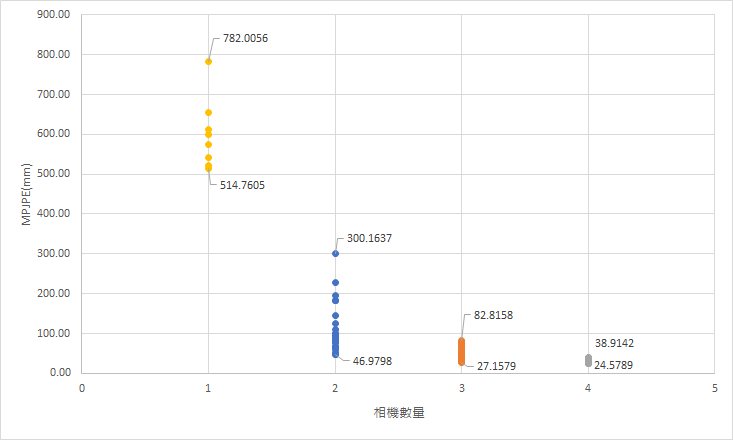
\includegraphics[width=\linewidth]{figure/ch3_fig_1to7cam.png}
   \caption[一台相機到七台相機的組合估計結果]{一台相機到七台相機的組合估計結果}
   \label{ch3_fig_1to7cam}
\end{figure}

% 跟位置討論有關的事情都先不放
% 另外列出每一相機數量的最佳表現及最差表現,如表~\ref{ch3_best_worst_camset},可以發現相機 1 皆有出現在最佳表現的結果中,而相機 2 皆有出現在最差表現的結果中,
% 因此推論相機 1 的位置較為適當。
% \begin{table}[!ht]
%    \caption[相機組合的最差及最佳表現]{相機組合的最差及最佳表現}
%    \centering
%    \label{ch3_best_worst_camset}
%    \setlength{\tabcolsep}{3pt}
%    \renewcommand\arraystretch{1.5}
%    \begin{tabular}{c|c|c|c|c}
%        & 1 cam & 2 cam & 3 cam & 4 cam \\ 
%       \midrule[2pt]
%       最差表現 & 2 & 25 & 257 & 2567 \\
%       最佳表現 & 1 & 18 & 137 & 1357 \\
%    \end{tabular}
% \end{table}

% \subsection{延伸討論}
% % 延伸討論,因為現在沒有一個比較好可以呈現這個結論的方式,所以先不放
% 由於目前文獻~\cite{zhang2020fusing}取用四台相機,因此若欲減少相機使用數量勢必會往三台相機及兩台相機的配置進行考量,
% 因此以下將進一步比較三台相機及兩台相機的估計結果,並進行討論。

% \subsubsection{方法}
% 將三台相機的估計結果依照兩台相機的配對進行平均,再與兩台相機的結果相減,以此方式觀察多一台相機的影響。
% 計算方式如算式~\ref{ch3_3camaveMin2cam}。
% \begin{equation}
%    \label{ch3_3camaveMin2cam}
%    \text{差值} = \text{ave}(\text{MPJPE}_{3 \text{ cam}})-\text{MPJPE}_{2 \text{ cam}}
% \end{equation}

% \subsubsection{結果}
% 以下表~\ref{ch3_ave_3cam_vs_2cam} 交互相機 18 為例,即將 128、138、148、158、168、178 六組相機配對的估計結果進行平均,
% 得 MPJPE = 34.5704,再與直接用兩台相機進行融合估計得到的 MPJPE = 46.9798 相減,得 12.4094。
% 由下表~\ref{ch3_ave_3cam_vs_2cam} 可知,相機 1 及相機 8 的配對再加上第三台相機較不會有顯著的改善,
% 且前三種配對 (即配對 18、配對 14、配對 48)的改善皆都落在約 10~15 mm 左右,
% 所以可以推斷,相機 1、4、8 三個位置,隨意取其中兩者可能是較適合擺放相機的位置。
% \begin{table}[!ht]
%    \caption[兩台相機與三台相機平均之比較]{兩台相機與三台相機平均之比較}
%    \centering
%    \label{ch3_ave_3cam_vs_2cam}
%    \setlength{\tabcolsep}{3pt}
%    \renewcommand\arraystretch{1.5}
%    \begin{tabular}{c|c|c|c}
%       交互相機 & $ave(MPJPE_{3 cam})$ & $MPJPE_{2 cam}$ & 差 \\
%       \midrule[2pt]
%       18 & 34.5704 & 46.9798 & 12.4094 \\
%       14 & 33.8308 & 47.4927 & 13.6619 \\
%       48 & 35.3844 & 52.3318 & 16.9474 \\
%       17 & 34.9321 & 58.7619 & 23.8298 \\ 
%       58 & 38.4382 & 64.6374 & 26.1993 \\
%       68 & 35.3408 & 63.7904 & 28.4496 \\
%       46 & 37.9318 & 66.8800 & 28.9481 \\  
%       47 & 38.0495 & 67.4949 & 29.4454 \\ 
%       16 & 35.3793 & 66.8653 & 31.4860 \\ 
%       15 & 39.8348 & 76.7795 & 36.9447 \\
%       78 & 39.5911 & 77.1948 & 37.6037 \\
%    \end{tabular}
% \end{table}

% 另外,若希望 $MPJPE_{2 cam}$ 低於 80 mm,則從兩台相機的估計結果(表~\ref{ch3_cameraset_2cam})挑選出 $MPJPE_{2 cam}$ 低於 80 mm 的結果,
% 並計算每一相機的出現次數,則可得出如下表~\ref{ch3_cam_occurrence} 的結果,觀察下表也可發現相機 1、8 的出現次數最高,
% 其次為相機 4 ,因此也可推斷相機 1、4、8 三個位置可能是較適合擺放相機的位置。
% \begin{table}[!ht]
%    \caption[兩台相機估計結果之每台相機的出現次數]{兩台相機估計結果之每台相機的出現次數}
%    \centering
%    \label{ch3_cam_occurrence}
%    \setlength{\tabcolsep}{3pt}
%    \renewcommand\arraystretch{1.5}
%    \begin{tabular}{c|c}
%       相機 & 出現次數 \\
%       \midrule[2pt]
%       1 & 5 \\
%       2 & 0 \\
%       3 & 0 \\
%       4 & 4 \\
%       5 & 2 \\
%       6 & 3 \\
%       7 & 3 \\
%       8 & 5 \\
%    \end{tabular}
% \end{table}

% ------------------------- 3.4 ------------------------- %
\section{結果可視化}
% 結果可視化介紹
% 分類成五個部分,分別用甚麼顏色表示

% ------------------------- 3.5 ------------------------- %
\section{小結}
% 本章架構
本章節首先介紹將會使用到的背景知識,像是透過希爾式肌肉模型來模擬肌肉,藉此理解肌肉的機械與生理特性,
而藉由 OpenSim 的協助,不但能快速建立肌肉骨骼模型,還可以執行正向動力學與肌肉計算控制等模擬,
且得到一個可信的結果,接下來介紹本研究的核心模擬——運動軌跡預測任務,後續的敏感度分析、最佳化過程與模型驗證,
皆是以預測任務為基礎來延伸,透過預測任務來檢視模型的表現,亦即預測誤差。
本研究透過敏感度分析來得知肌肉與任務之間的關係,藉此挑選合適的任務集作為參數評估輸入,
搭配最佳化演算法來進行參數估計,其中多組預測任務具有讓目標函數更加明確的功用,避免參數不具識別性的原因,
掉入至局部最小值結果當中,最終透過間接方法來驗證模型的正確性。

% 應用
該研究方法之應用可分為兩種討輪,第一是模擬研究,即為本研究使用之方法,透過純模擬研究來檢視該方法的可行性,
優點是其具有明確答案可供參考,且無需考慮量測造成的不確定性,在進入到實際應用前,也必須先確認模擬研究是可執行的;
第二種則是實際應用,其可透過 EMG 與動作捕捉系統來達成,藉由 EMG 量測肌肉訊號作為輸入,
動作捕捉系統量測運動軌跡作為輸出之結果比較,兩者結合並搭配本研究之最佳化方法,即可達成肌肉之參數估計,
但存在龐大的量測不確定性情況下,由於微小的軌跡偏離,即會造成肌肉參數的變動與抗衡,
縱使估計出肌肉參數,其結果之正確性仍有待商榷,因此於現今之科技發展,要達成實際應用仍有一段距離。

% 下一章節
本章節主要介紹論文之研究方法,下章節會以實際模型與動作進行討論,藉由上方所提及之方法與流程,
針對模型進行肌肉參數評估的前置作業與套用說明。

\clearpage
% \chapter{系統驗證之實驗結果與討論}
\chapter{結果與討論}
\fontsize{12pt}{18pt}\selectfont %字體大小,行距

% ------------------------- 4.0 ------------------------- %
% 概述
本章節首先透過先前學者們提出的資料集與影像辨識融合 IMU 方法,探討減少相機使用數量對於人體姿態估計精準度的影響,以最大程度的減少量測設備的成本及架設時間。此外,本研究提出使用影像辨識及三角測量計算方法建立三維人體模型,並使用先前學者提出的資料集進行驗證。最後,本研究將透過蹲站、開合跳、折返跑、熱身運動等實驗,驗證融合 IMU 資訊是否對於影像辨識重建人體姿態有所改善。

% ------------------------- 4.1 ------------------------- %
% \section{探討減少相機使用數量對於人體姿態估計精準度的影響實驗結果與討論}\label{ch4_sec_cameraset}
\section{探討減少相機使用數量對於人體姿態估計精準度的影響實驗}\label{ch4_sec_cameraset}
% 實驗結果
% 經過上述七類情況之實驗後,得到的 MPJPE 結果如以下所示。
\subsection{實驗設定}
本研究使用使用學者 Zhe Zhang 等人提出的感測器融合方法進行影像與 IMU 資訊的融合~\cite{Zhang_2020_CVPR},沿用其文獻中的所有實驗設定,包括相機校正、三維人體模型建立、時間同步及空間校正、使用 8 個 IMU,分別為左右上臂、左右前臂、左右大腿、左右小腿,僅更改使用相機的數量及組合,每一結果皆可計算出 MPJPE 數值。本研究將進行 7 種不同的實驗設定,分別為使用一台相機、使用兩台相機,以此類推至使用七台相機,並探討不同相機數量對人體姿態估計的影響。

\clearpage

\subsection{實驗結果與誤差評估}
\subsubsection{使用一台相機及八個 IMU 進行人體姿態重建實驗結果}
將圖~\ref{ch3_fig_cameraset_totalcap} 中的相機任選一台進行估計,共計有 8 種估計結果,每一結果皆可計算出 MPJPE 數值,
MPJPE 數值計算結果如表~\ref{ch3_cameraset_1cam} 所示,可以發現無論選擇哪一個位置的相機,其估計誤差皆超過 500 (mm)。
標準差為 87.6016 (mm),平均值為 599.8855 (mm)。
% 因此本研究認為只使用一台相機進行估計是不可行的,至少需使用兩台相機進行量測。
\begin{table}[!ht]
   \caption[一台相機組合與其估計結果誤差]{一台相機組合與其估計結果誤差}
   \centering
   \label{ch3_cameraset_1cam}
   \setlength{\tabcolsep}{3pt}
   \renewcommand\arraystretch{1.5}
   \resizebox{\textwidth}{!}{
   \begin{tabular}{
   >{\columncolor[HTML]{E7E6E6}}c |c|
   >{\columncolor[HTML]{E7E6E6}}c |c|
   >{\columncolor[HTML]{E7E6E6}}c |c|
   >{\columncolor[HTML]{E7E6E6}}c |c}
   \toprule
      相機編號 & MPJPE & 相機編號 & MPJPE & 相機編號 & MPJPE & 相機編號 & MPJPE \\
      \midrule
      1	& 514.76 & 2 & 782.01 & 3 & 611.84 & 4 & 520.97 \\
      5	& 653.96 & 6 & 573.41 & 7 & 599.78 & 8 & 542.36 \\
   \bottomrule
   \end{tabular}}
\end{table}
\clearpage

\subsubsection{使用兩台相機及八個 IMU 進行人體姿態重建實驗結果}
將圖~\ref{ch3_fig_cameraset_totalcap} 中的相機任選兩台進行排列組合,共計有 28 種組合方式之估計結果,每一結果皆可計算出 MPJPE 數值,
MPJPE 數值計算結果如表~\ref{ch3_cameraset_2cam} 所示,其中最佳組合方式為相機 18,其 MPJPE 數值為 46.9798 (mm);
而最差組合方式為相機 25,其 MPJPE 數值為 300.1637 (mm)。標準差為 61.7928 (mm),平均值為 109.8694 (mm)。
經由平均值可以發現兩台相機的姿勢估計表現相對一台相機的姿勢估計表現有大幅度的進步,進步幅度約為 500 (mm);
但是由標準差可知兩台相機的姿勢估計結果仍不穩定。
% 經由結果可以發現相機的擺放位置對估計結果影響甚鉅,若位置選擇得宜,估計結果將會相當準確,反之則會有較大的誤差。
\begin{table}[!ht]
   \caption[兩台相機組合與其估計結果誤差]{兩台相機組合與其估計結果誤差}
   \centering
   \label{ch3_cameraset_2cam}
   \setlength{\tabcolsep}{3pt}
   \renewcommand\arraystretch{1.5}
   \resizebox{\textwidth}{!}{
   \begin{tabular}{
   >{\columncolor[HTML]{E7E6E6}}c |c|
   >{\columncolor[HTML]{E7E6E6}}c |c|
   >{\columncolor[HTML]{E7E6E6}}c |c|
   >{\columncolor[HTML]{E7E6E6}}c |c}
   \toprule
      相機組合 & MPJPE & 相機組合 & MPJPE & 相機組合 & MPJPE & 相機組合 & MPJPE \\
      \midrule
      12 & 194.4957 & 13 & 81.9440 & 14 & 47.4927 & 15 & 76.7795 \\
      16 & 66.8653 & 17 & 58.7619 & 18 & 46.9798 & & \\
      \midrule
      23 & 227.5722 & 24 & 182.6378 & 25 & 300.1637 & 26 & 183.0773 \\
      27 & 181.6520 & 28 & 145.2458 & & & &\\
      \midrule
      34 & 99.3426 & 35 & 109.4178 & 36 & 92.7550 & 37 & 97.7435 \\
      38 & 81.3640 & & & & & &\\
      \midrule
      45 & 87.4750 & 46 & 66.8800 & 47 & 67.4949 & 48 & 52.3318 \\
      \midrule
      56 & 126.3387 & 57 & 95.1469 & 58 & 64.6374 & &\\
      \midrule
      67 & 100.7632 & 68 & 63.7904 & & & &\\
      \midrule
      78 & 77.1948 & & & & & &\\
   \bottomrule
   \end{tabular}}
\end{table}
\clearpage

\subsubsection{使用三台相機及八個 IMU 進行人體姿態重建實驗結果}
將圖~\ref{ch3_fig_cameraset_totalcap} 中的相機任選三台進行排列組合,共計有 56 種組合方式之估計結果,每一結果皆可計算出 MPJPE 數值,
MPJPE 數值計算結果如表~\ref{ch3_cameraset_3cam} 所示,其中最佳組合方式為相機 137,其 MPJPE 數值為 27.1579 (mm);
而最差組合方式為相機 257,其 MPJPE 數值為 82.8158 (mm)。標準差為 13.8423 (mm),平均值為 42.9001 (mm)。
經由平均值可以發現:相較兩台相機的姿勢估計結果,三台相機的姿勢估計結果準確性仍有明顯提升,進步幅度約為 60 (mm);
由標準差可以知道三台相機的姿勢估計結果漸趨穩定。
% 但只要位置恰當,僅用三台相機也可以有四台相機的表現水準。
\begin{table}[!ht]
   \caption[三台相機組合與其估計結果誤差]{三台相機組合與其估計結果誤差}
   \centering
   \label{ch3_cameraset_3cam}
   \setlength{\tabcolsep}{3pt}
   \renewcommand\arraystretch{1.5}
   \resizebox{\textwidth}{!}{
   \begin{tabular}{
   >{\columncolor[HTML]{E7E6E6}}c |c|
   >{\columncolor[HTML]{E7E6E6}}c |c|
   >{\columncolor[HTML]{E7E6E6}}c |c|
   >{\columncolor[HTML]{E7E6E6}}c |c|
   >{\columncolor[HTML]{E7E6E6}}c |c}
   \toprule
      相機組合 & MPJPE & 相機組合 & MPJPE & 相機組合 & MPJPE & 相機組合 & MPJPE & 相機組合 & MPJPE \\
      \midrule
      123 & 41.8538 & 124 & 43.2544 & 125 & 70.4747 & 126 & 41.7470 & 127 & 54.5721 \\
      128 & 46.7714 & & & & & & & & \\
      134 & 30.9862 & 135 & 29.0275 & 136 & 33.6116 & 137 & 27.1579 & 138 & 29.9961 \\
      145 & 34.4860 & 146 & 32.7227 & 147 & 29.9785 & 148 & 31.5573 & & \\
      156 & 38.3802 & 157 & 33.2107 & 158 & 33.4297 & & & & \\
      167 & 32.4098 & 168 & 33.4044 & 178 & 32.2636 & & & & \\
      \midrule
      234 & 52.0193 & 235 & 76.4435 & 236 & 52.6657 & 237 & 65.5297 & 238 & 44.5936 \\
      245 & 76.6047 & 246 & 42.4841 & 247 & 54.8719 & 248 & 45.2496 & & \\
      256 & 74.8608 & 257 & 82.8158 & 258 & 62.4336 & & & & \\
      267 & 58.7578 & 268 & 39.2619 & 278 & 62.7102 & & & & \\
      \midrule
      345 & 35.9928 & 346 & 42.7418 & 347 & 35.2381 & 348 & 33.5695 & & \\
      356 & 42.9933 & 357 & 35.1894 & 358 & 29.6995 & & & & \\
      367 & 40.0411 & 368 & 35.8360 & 378 & 34.9221 & & & & \\
      \midrule
      456 & 40.0658 & 457 & 37.2030 & 458 & 32.7289 & & & & \\
      467 & 35.6906 & 468 & 33.8860 & 478 & 35.3151 & & & & \\
      \midrule
      567 & 41.5287 & 568 & 34.8289 & 578 & 37.5083 & & & & \\
      \midrule
      678 & 34.8273 & & & & & & & & \\
   \bottomrule
   \end{tabular}}
\end{table}
\clearpage

\subsubsection{使用四台相機及八個 IMU 進行人體姿態重建實驗結果}
將圖~\ref{ch3_fig_cameraset_totalcap} 中的相機任選四台進行排列組合,共計有 70 種組合方式之估計結果,每一結果皆可計算出 MPJPE 數值,
MPJPE 數值計算結果如表~\ref{ch3_cameraset_4cam} 所示,其中最佳組合方式為相機 1357,其 MPJPE 數值為 24.5789 (mm);
而最差組合方式為相機 2567,其 MPJPE 數值為 38.9142 (mm)。標準差為 3.6860 (mm),平均值為 31.0114 (mm)。
經由平均值可以發現,四台相機的姿勢估計結果相對三台相機的姿勢估計結果有進一步提升,進步幅度約為 10 (mm),
相較兩台相機與三台相機的進步幅度有逐漸平穩的趨勢;
而由標準差可以知道四台相機組合的表現都相當穩定,無論如何選擇都不會有太大的影響。
\begin{table}[!ht]
   \caption[四台相機組合與其估計結果誤差]{四台相機組合與其估計結果誤差}
   \centering
   \label{ch3_cameraset_4cam}
   \setlength{\tabcolsep}{3pt}
   \renewcommand\arraystretch{1.5}
   \resizebox{\textwidth}{!}{
   \begin{tabular}{
   >{\columncolor[HTML]{E7E6E6}}c |c|
   >{\columncolor[HTML]{E7E6E6}}c |c|
   >{\columncolor[HTML]{E7E6E6}}c |c|
   >{\columncolor[HTML]{E7E6E6}}c |c|
   >{\columncolor[HTML]{E7E6E6}}c |c}
   \toprule
      相機組合 & MPJPE & 相機組合 & MPJPE & 相機組合 & MPJPE & 相機組合 & MPJPE & 相機組合 & MPJPE \\
      \midrule
      1234 & 30.9409 & 1235 & 28.8549 & 1236 & 30.3748 & 1237 & 28.8213 & 1238 & 31.1560 \\
      1245 & 33.1706 & 1246 & 31.5377 & 1247 & 32.1031 & 1248 & 33.6613 &            &         \\
      1256 & 34.5089 & 1257 & 34.6787 & 1258 & 35.2625 &            &         &            &         \\
      1267 & 31.7009 & 1268 & 33.0636 & 1278 & 34.6861 &            &         &            &         \\
      1345 & 26.9753 & 1346 & 28.2925 & 1347 & 25.4715 & 1348 & 26.7584 &            &         \\
      1356 & 27.7651 & 1357 & 24.5789 & 1358 & 25.8578 &            &         &            &         \\
      1367 & 26.3845 & 1368 & 26.9445 & 1378 & 26.1466 &            &         &            &         \\
      1456 & 29.9311 & 1457 & 26.6848 & 1458 & 27.9429 &            &         &            &         \\
      1467 & 26.8121 & 1468 & 27.5472 & 1478 & 27.1979 &            &         &            &         \\
      1567 & 27.5824 & 1568 & 29.1892 & 1578 & 27.4552 & 1678 & 27.8378 &            &         \\
      \midrule
      2345 & 34.0972 & 2346 & 36.5508 & 2347 & 36.7314 & 2348 & 33.7047 &            &         \\
      2356 & 35.6585 & 2357 & 36.3698 & 2358 & 30.8585 &            &         &            &         \\
      2367 & 36.8662 & 2368 & 32.6160 & 2378 & 34.8430 &            &         &            &         \\
      2456 & 35.6440 & 2457 & 37.1359 & 2458 & 33.4067 &            &         &            &         \\
      2467 & 35.8266 & 2468 & 33.2654 & 2478 & 36.6081 &            &         &            &         \\
      2567 & 38.9142 & 2568 & 33.7187 & 2578 & 38.7211 & 2678 & 34.3506 &            &         \\
      \midrule
      3456 & 32.4429 & 3457 & 27.7338 & 3458 & 27.6554 &            &         &            &         \\
      3467 & 31.0735 & 3468 & 29.9925 & 3478 & 27.9168 &            &         &            &         \\
      3567 & 29.2876 & 3568 & 28.3170 & 3578 & 26.8460 & 3678 & 29.4004 &            &         \\
      \midrule
      4567 & 29.8717 & 4568 & 29.7963 & 4578 & 28.2055 & 4678 & 28.9104 & 5678 & 29.5824 \\
   \bottomrule
   \end{tabular}}
\end{table}
\clearpage

\subsubsection{使用五台相機及八個 IMU 進行人體姿態重建實驗結果}
將圖~\ref{ch3_fig_cameraset_totalcap} 中的相機任選三台進行排列組合,共計有 56 種組合方式之估計結果,每一結果皆可計算出 MPJPE 數值,MPJPE 數值計算結果如表~\ref{ch3_cameraset_5cam} 所示,其中最佳組合方式為相機 13578,其 MPJPE 數值為 23.9568 (mm);而最差組合方式為相機 23467,其 MPJPE 數值為 32.1120 (mm)。標準差為 2.0034 (mm),平均值為 27.6608 (mm)。經由平均值可以發現:相較四台相機的姿勢估計結果,五台相機的姿勢估計結果並無明顯提升,進步幅度約為 4 (mm);由標準差可以知道五台相機的姿勢估計結果十分集中,且將平均值與四台相機的平均值相比並無明顯進步。
\begin{table}[!ht]
   \caption[五台相機組合與其估計結果誤差]{五台相機組合與其估計結果誤差}
   \centering
   \label{ch3_cameraset_5cam}
   \setlength{\tabcolsep}{3pt}
   \renewcommand\arraystretch{1.5}
   \resizebox{\textwidth}{!}{
   \begin{tabular}{
   >{\columncolor[HTML]{E7E6E6}}c |c|
   >{\columncolor[HTML]{E7E6E6}}c |c|
   >{\columncolor[HTML]{E7E6E6}}c |c|
   >{\columncolor[HTML]{E7E6E6}}c |c|
   >{\columncolor[HTML]{E7E6E6}}c |c}
   \toprule
      相機組合 & MPJPE & 相機組合 & MPJPE & 相機組合 & MPJPE & 相機組合 & MPJPE & 相機組合 & MPJPE \\
      \midrule
      12345 & 27.2222 & 12346 & 28.7270 & 12347 & 27.2410 & 12348 & 28.1424 & 12356 & 27.5630  \\
      12357 & 25.4345 & 12358 & 26.9508 & 12367 & 27.4309 & 12368 & 27.9631 & 12378 & 27.5871  \\
      12456 & 29.2157 & 12457 & 27.4585 & 12458 & 29.1856 & 12467 & 28.0690 & 12468 & 28.8999  \\
      12478 & 28.9294 & 12567 & 28.2794 & 12568 & 29.9585 & 12578 & 29.0917 & 12678 & 29.1141  \\
      13456 & 26.5308 & 13457 & 24.2506 & 13458 & 24.7973 & 13467 & 25.4456 & 13468 & 25.5140  \\
      13478 & 24.5152 & 13567 & 24.7163 & 13568 & 25.2622 & 13578 & 23.9568 & 13678 & 25.0847  \\
      14567 & 25.6222 & 14568 & 26.3839 & 14578 & 25.2386 & 14678 & 25.3628 & 15678 & 26.0199  \\
      \midrule
      23456 & 31.3515 & 23457 & 28.8724 & 23458 & 28.4882 & 23467 & 32.1120 & 23468 & 30.4884  \\
      23478 & 29.8341 & 23567 & 29.8954 & 23568 & 28.7786 & 23578 & 27.9967 & 23678 & 30.1241  \\
      24567 & 30.4360 & 24568 & 30.1827 & 24578 & 29.4012 & 24678 & 30.1792 & 25678 & 30.1283  \\
      \midrule
      34567 & 27.4939 & 34568 & 27.0215 & 34578 & 25.1997 & 34678 & 27.0385 & 35678 & 26.0327  \\
      \midrule
      45678 & 26.7827 & ~ & ~ & ~ & ~ & ~ & ~ & ~ &   \\
   \bottomrule
   \end{tabular}}
\end{table}

\clearpage

\subsubsection{使用六台相機、七台相機與八個 IMU 進行人體姿態重建實驗結果}
由於六台相機與七台相機之估計結果皆與四台相機及五台相機的估計結果相近,因此將於附錄~\ref{appendix:6cam7cam} 列出。
六台相機姿勢估計誤差之標準差為 1.3281 (mm),平均值為 25.9980 (mm),
七台相機姿勢估計誤差之標準差為 0.8525 (mm),平均值為 24.9272 (mm)。
將兩者的標準差及平均值與五台相機的標準差及平均值進行比較,
可以發現六台相機及七台相機的表現皆與五台相機的表現結果相近,無大幅度的進步,
因此推測增加相機數量以改善姿勢估計誤差的策略存在極限,使用四台相機即可,
再繼續增加相機數量無法顯著改善估計準確性。

\clearpage

\subsection{結論}
% 結果介紹與討論
將以上結果的平均及標準差整理如表~\ref{ch3_cameraset_summary},可以發現隨著相機數量的增加,MPJPE 數值有明顯的下降趨勢,且由標準差可以知道,隨著相機數量的增加,MPJPE 數值的穩定性也有明顯的提升。

\begin{table}[ht]
   \caption{MPJPE 數值的平均及標準差}
   \label{ch3_cameraset_summary}
   \setlength{\tabcolsep}{3pt}
   \renewcommand\arraystretch{1.5}
   \resizebox{\textwidth}{!}{
   \begin{tabular}{c|S|S|S|S|S|S|S}
   \toprule
    & 一台相機 & 二台相機 & 三台相機 & 四台相機 & 五台相機 & 六台相機 & 七台相機 \\
   \midrule
   平均 (mm) & 599.89 & 109.87 & 42.90 & 31.01 & 27.66 & 26.00 & 24.93 \\
   標準差 (mm) & 87.60 & 61.79 & 13.84 & 3.69 & 2.00 & 1.33 & 0.85 \\
   \bottomrule
   \end{tabular}}
\end{table}

將一台相機到七台相機的全部 MPJPE 數值繪製成圖~\ref{ch3_fig_1to7cam},
可以發現相機數量從一台增加到四台時,MPJPE 數值隨著相機數量的增加有明顯下降的趨勢,從四台相機開始,MPJPE 數值的下降幅度逐漸減緩,因此可以推斷,當相機數量增加到四台時,MPJPE 數值的表現已經相當穩定,且相機數量增加到五台以上時,MPJPE 數值的表現並不會有太大的改善。另外,若觀察每一相機數量的最佳表現 (即 MPJPE 數值的最小值),可以發現兩台相機及三台相機的最佳表現皆有到達誤差 50 (mm) 以下,平均誤差約 40 \textasciitilde\ 100 (mm),所以,若希望盡可能減少相機數量,且容許誤差 100 (mm),則可以選擇兩台相機或三台相機進行姿勢估計,因此,綜上所述可推斷,為增加實驗架設方便性,減少相機數量是可考慮的選擇。
% 所以,若要達到最佳的姿勢估計結果,相機數量應選擇四台即可。
% MPJPE 數值約都在 20\textasciitilde40 mm 左右,只是如果三台相機的組合適當的話,結果並不會比四台相機的結果差。
\begin{figure}[!ht]
   \centering
   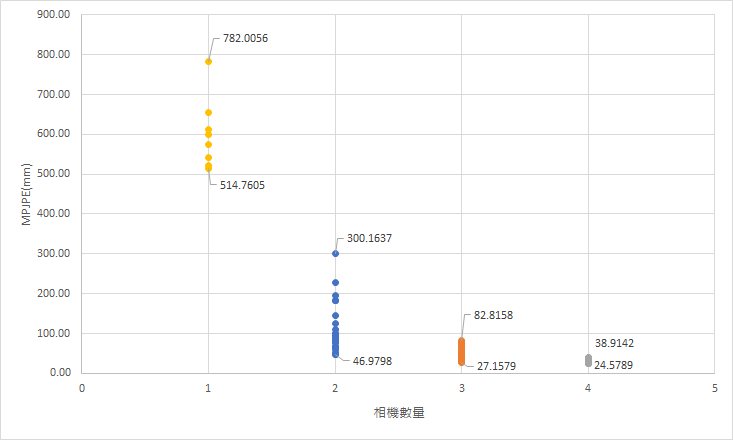
\includegraphics[width=13cm]{figure/ch3_fig_1to7cam.png}
   \caption[一台相機到七台相機的組合估計結果]{一台相機到七台相機的組合估計結果}
   \label{ch3_fig_1to7cam}
\end{figure}

\clearpage

% ------------------------- 4.2 ------------------------- %
% \section{個人化三維人體模型建立實驗結果與討論}\label{ch4_skeleton_exp}
\section{以影像辨識方法建立個人化三維人體模型}\label{ch4_skeleton_exp}
% 實驗設定;實驗執行;結果與討論
% 在章節~\ref{ch3_skeleton_method} 中已詳細描述了個人化三維人體模型建立的方法,
% 本節使用 TotalCapture Dataset~\cite{Trumble:BMVC:2017} 提供的影片資料及相機校正數據,
% 嘗試建立影片中受試者的個人化三維人體模型,並進行比較及討論。

\subsection{實驗設定}
% 把 total capture dataset s1 系列做完
% FIXME:只取九組的原因
本章節使用 TotalCapture Dataset ~\cite{Trumble:BMVC:2017} 提供的 s1\_acting1 \textasciitilde\ s1\_acting3、s1\_freestyle1 \textasciitilde\ s1\_freestyle3、s1\_rom1 \textasciitilde\ s1\_rom3 共九組影片資料及相機校正資料進行實驗,每組實驗皆取用 TotalCapture Dataset  中,與本實驗視角最為相近的相機 1 與相機 8 之影像資料、兩台相機的校正資訊,以及 .bvh 檔案中 HIERARCHY 部分提供的 Vicon 三維人體模型資訊 (此資訊可由 Vicon 量測而得,因此以下將稱為 Vicon 三維人體模型)。首先,利用影像資料進行 OpenPose 影像辨識,再使用 Pose2Sim 進行相機校正及三角測量計算,建立出個人化三維人體模型。最後,由於每個檔案只有前 60 幀為 T-pose 動作,因此取前 60 幀的資訊,計算個人化三維人體模型的平均四肢長度,並與 Vicon 三維人體模型的四肢長度進行比較。

\subsection{實驗結果與誤差評估}
% 個人化三維人體模型建立結果與驗證
% 分別評估四肢的誤差,然後再綜合再一起評估,總結誤差大概在多少內
分別計算出自行建立個人化三維人體模型的四肢長度及 Vicon 三維人體模型長度後,將兩者相減並取絕對值得到誤差,再計算平均誤差,結果如表~\ref{ch3_skeleton_compare} 所示,可以發現自行建立個人化三維人體模型之四肢長度與 Vicon 三維人體模型之四肢長度相當接近,整體平均誤差為 25.75 (mm)。本研究推斷,此項誤差可能來自 OpenPose 自身影像辨識造成的誤差,以及相機校正及三角測量的誤差。
% \sout{因此,若要進一步提升個人化三維人體模型的精確度,可能需要改善 OpenPose 的影像辨識精度,或是改善相機校正及三角測量的精確度。}

\begin{table}[!ht]
   \caption[個人化三維人體模型建立結果與比較(mm)]{個人化三維人體模型建立結果與比較(mm)}
   \centering
   \label{ch3_skeleton_compare}
   \setlength{\tabcolsep}{3pt}
   \renewcommand\arraystretch{1.5}
   \resizebox{\textwidth}{!}{
    \begin{tabular}{c|S|S|S|S|S|S|S|S|S||S}
      & {s1\_acting1} & {s1\_acting2} & {s1\_acting3} & {s1\_freestyle1} & {s1\_freestyle2} & {s1\_freestyle3} & {s1\_rom1} & {s1\_rom2} & {s1\_rom3} & {average} \\
      \midrule[1.5pt]
      右大腿 & 15.59 & 16.80 & 5.87 & 27.96 & 24.07 & 18.20 & 9.79 & 12.21 & 1.56 & 14.67 \\
      右小腿 & 20.43 & 0.75 & 8.96 & 11.48 & 12.74 & 2.58 & 19.07 & 20.56 & 8.64 & 11.69 \\
      左大腿 & 20.14 & 23.35 & 14.83 & 34.84 & 25.48 & 29.73 & 18.88 & 15.36 & 24.72 & 23.04 \\
      左小腿 & 3.48 & 7.87 & 16.62 & 15.05 & 12.44 & 15.55 & 12.30 & 3.26 & 3.26 & 9.98 \\
      右上臂 & 37.19 & 39.60 & 43.28 & 76.66 & 59.65 & 34.13 & 59.45 & 29.43 & 32.08 & 45.72 \\
      右前臂 & 4.06 & 20.92 & 14.48 & 59.10 & 37.33 & 10.66 & 36.69 & 4.39 & 13.86 & 22.39 \\
      左上臂 & 47.64 & 50.88 & 51.33 & 41.44 & 48.94 & 51.42 & 36.56 & 50.45 & 53.24 & 47.99 \\
      左前臂 & 30.76 & 24.33 & 36.55 & 19.80 & 29.58 & 34.79 & 22.61 & 35.96 & 40.44 & 30.54 \\
      \midrule[1.5pt]
      Average & 22.41 & 23.06 & 23.99 & 35.79 & 31.28 & 24.63 & 26.92 & 21.45 & 22.22 & 25.75 \\
   \end{tabular}}
\end{table}

\subsection{結論}
% 結論
由以上誤差評估可知,本方法的整體平均誤差約為 25.75 (mm),若僅用於建立三維人體模型、評估人體全身姿勢,不進行複雜動作的量測,使動作產生許多遮擋問題,或是延伸應用於評估手指姿勢等細微動作,則此誤差並不會造成誤判的影響,因此證明本方法確實可應用於建立三維人體模型,作為將 IMU 朝向資訊轉換為位置資訊的媒介。

% ------------------------- 4.3 ------------------------- %
% \section{使用影像辨識估計姿態}
% % 單獨 heatmap 的結果
% \subsection{實驗設定}
% % 實驗設定
% 本章節將自行蒐集的資料輸入進學者 Zhe Zhang 等人提出的感測器融合方法中進行人體姿態重建~\cite{Zhang_2020_CVPR}。該方法中包含兩個主要流程,一為影像辨識,二為影像辨識結果融合 IMU 資訊,本章節僅使用影像辨識進行人體姿態重建,不進行 IMU 資訊融合。使用的影像辨識方法為文獻~\cite{Xiao_2018_ECCV} 中,學者 Bin Xiao 等人提出的方法,並套用 Zhe Zhang 等人訓練的 $occlusion\_person\_8view.pth$ 模型進行影像辨識~\cite{zhang2020adafuse},取得記錄關節點於影像中位置的初步熱圖後,使用三角測量方法計算關節點的三維位置,進而重建人體姿態。

% % \subsection{實驗執行}
% % % 實驗執行

% \subsection{實驗結果與誤差評估}
% \subsubsection*{T-pose實驗結果}
% % 用pose_41、273
% 使用影像辨識融合 IMU 資訊的 T-pose 重建結果如圖~\ref{ch4_fig_Tpose_noimu} 所示,(a)、(b) 為同一時刻點的 cam01 的真實影像及 cam02 的真實影像,(c) 為人體重建結果;(c)、(d) 為同一時刻點的 cam01 的真實影像及 cam02 的真實影像,(e) 為人體重建結果。可以發現,在第二個時刻的 T-pose 人體重建結果與真實人體姿態有些出入。
% \begin{figure}[!ht]
%    \centering
%    \begin{minipage}{.3\textwidth}
%      \centering
%      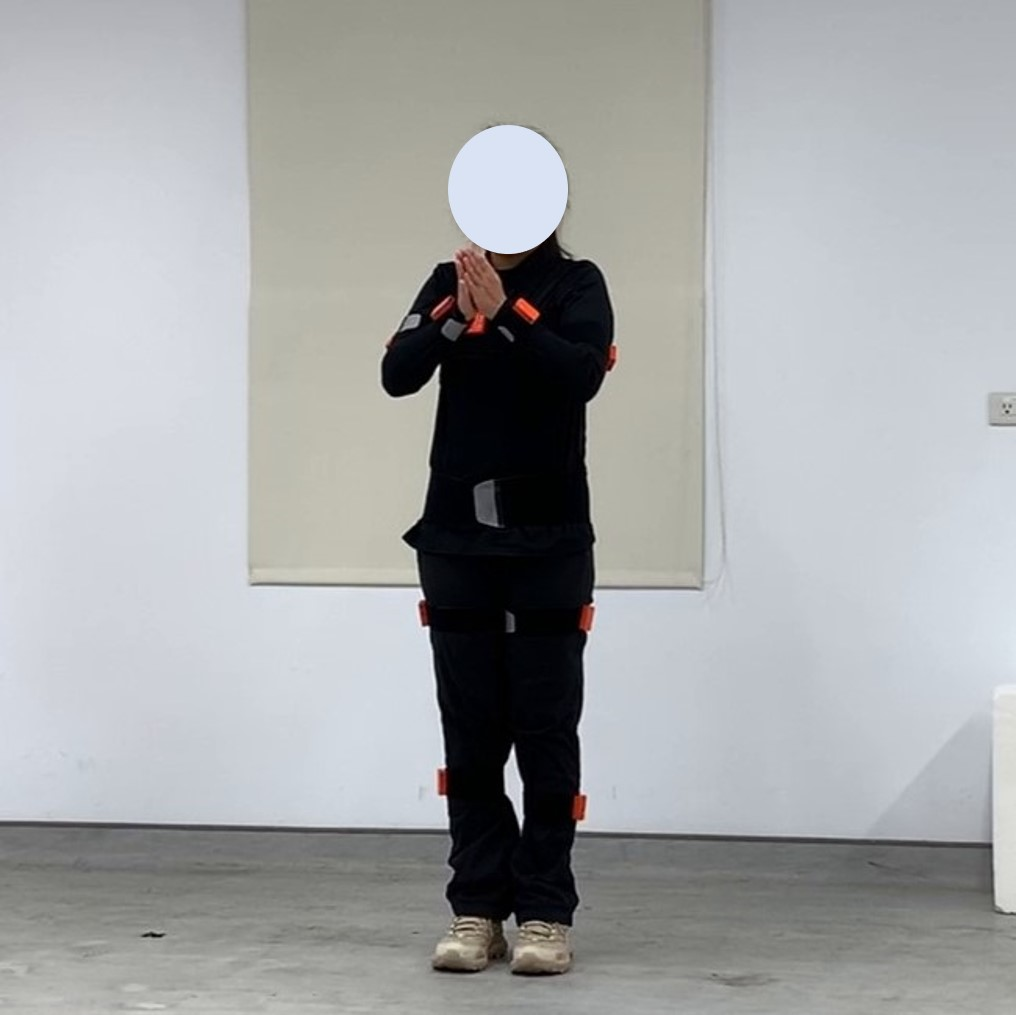
\includegraphics[width=\linewidth]{figure/ch4_fig_tpose_cam01_no1.jpg}
%      \caption*{(a) cam01 真實影像}
%    \end{minipage}%
%    \begin{minipage}{.3\textwidth}
%       \centering
%       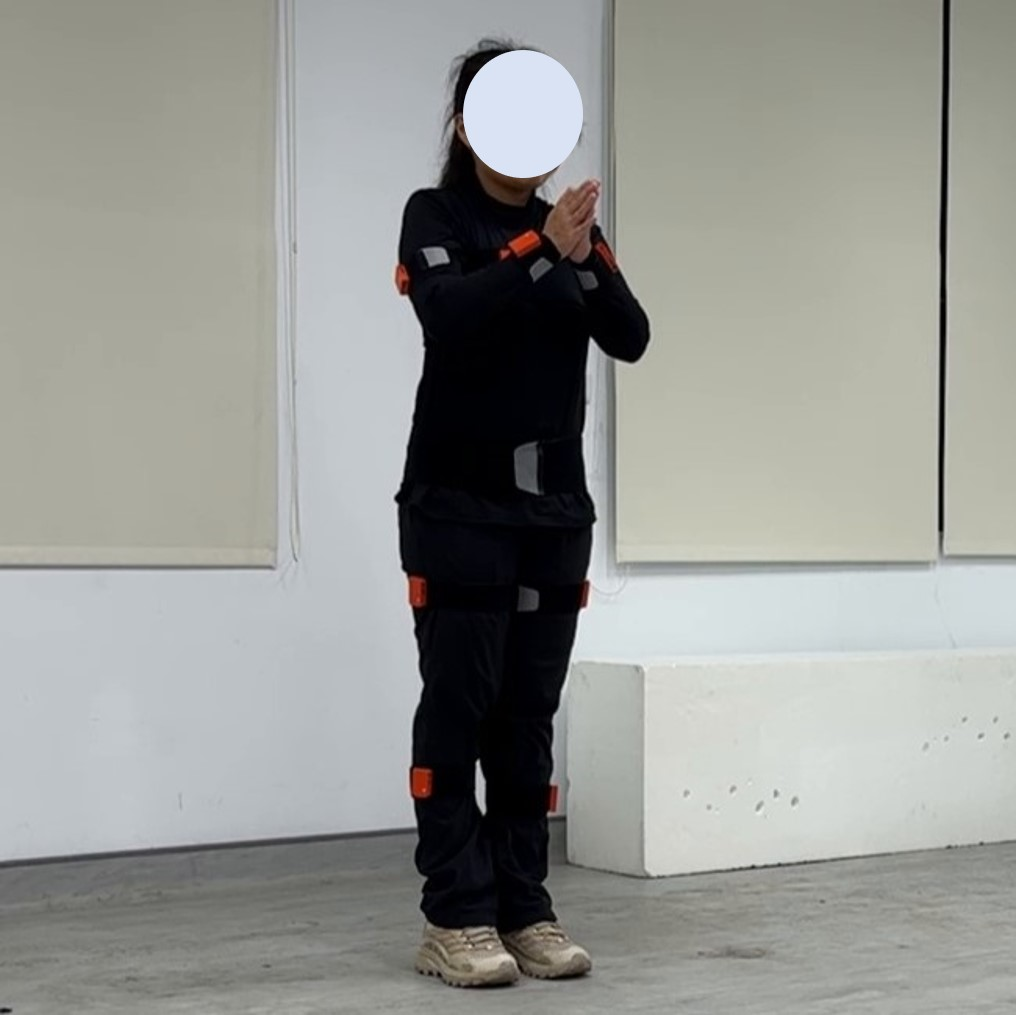
\includegraphics[width=\linewidth]{figure/ch4_fig_tpose_cam02_no1.jpg}
%       \caption*{(b) cam02 真實影像}
%    \end{minipage}%
%    \begin{minipage}{.3\textwidth}
%       \centering
%       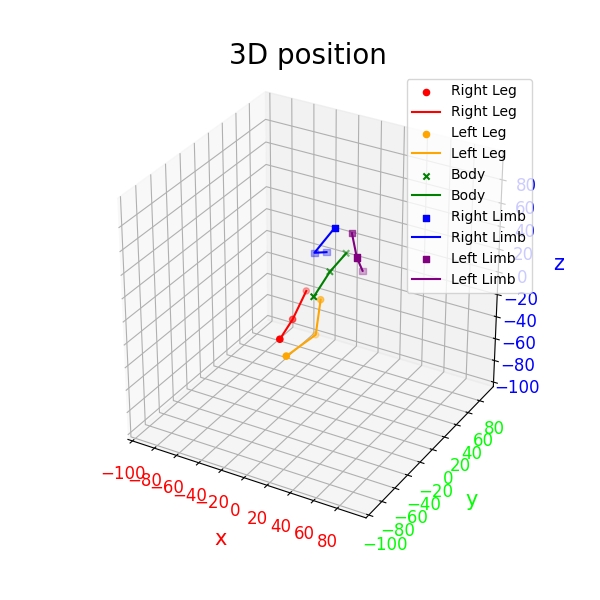
\includegraphics[width=\linewidth]{figure/ch4_fig_tpose_result_no1.png}
%       \caption*{(c) 重建結果}
%    \end{minipage}
%    \begin{minipage}{.3\textwidth}
%      \centering
%      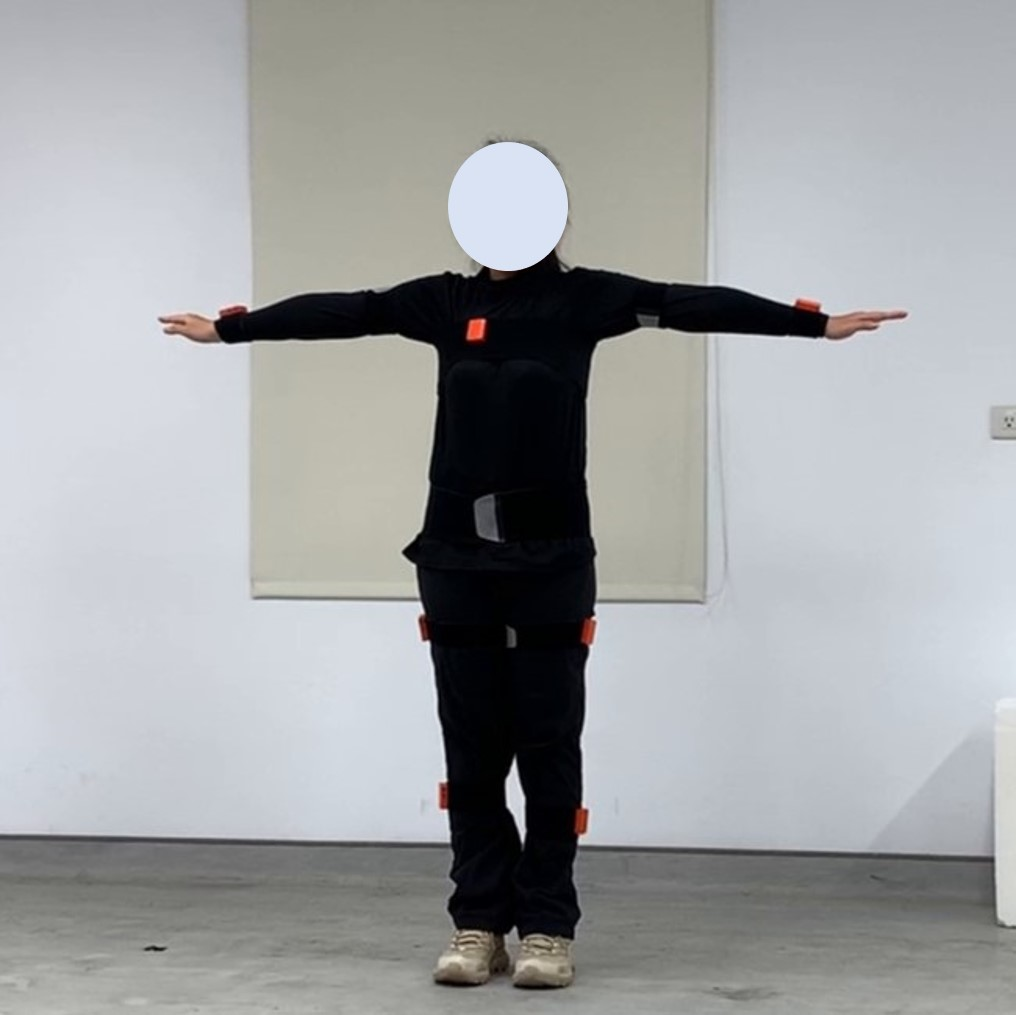
\includegraphics[width=\linewidth]{figure/ch4_fig_tpose_cam01_no2.jpg}
%      \caption*{(d) cam01 真實影像}
%    \end{minipage}%
%    \begin{minipage}{.3\textwidth}
%       \centering
%       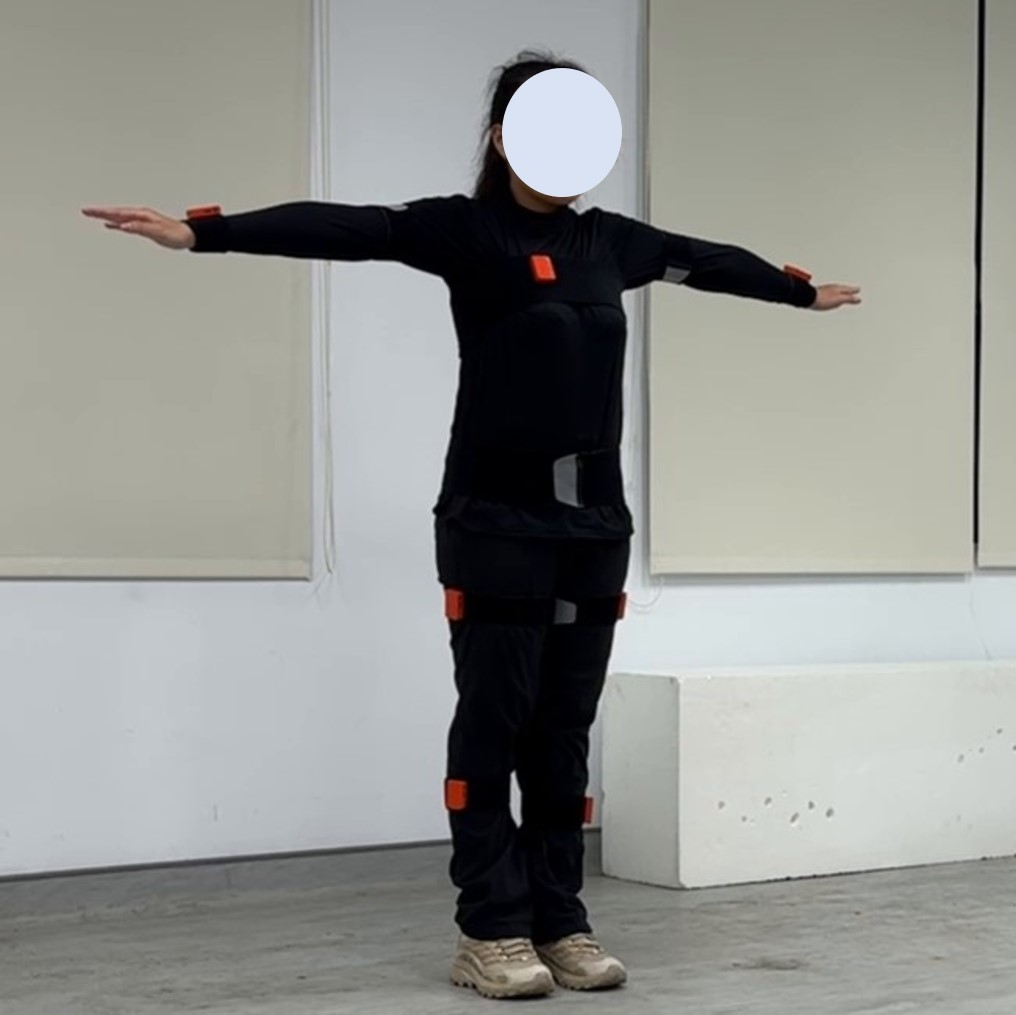
\includegraphics[width=\linewidth]{figure/ch4_fig_tpose_cam02_no2.jpg}
%       \caption*{(e) cam02 真實影像}
%     \end{minipage}%
%     \begin{minipage}{.3\textwidth}
%       \centering
%       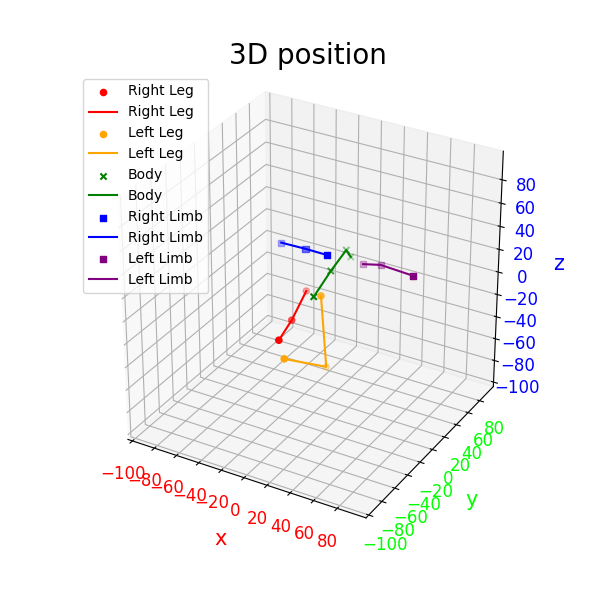
\includegraphics[width=\linewidth]{figure/ch4_fig_tpose_result_no2.png}
%       \caption*{(f) 重建結果}
%     \end{minipage}
%    \caption[僅使用影像辨識進行 T-pose 重建結果]{僅使用影像辨識進行 T-pose 重建結果}
%    \label{ch4_fig_Tpose_noimu}
% \end{figure}

% \subsubsection*{T-pose 誤差評估}
% T-pose 實驗總計有 318 幀,每一幀皆估計出人體姿態,每 20 幀進行一次採樣,共計 16 個樣本點進行評估及驗證,
% % 結果如表~\ref{ch4_Tpose_result_noimu} 所示,
% 可以發現,T-pose 實驗中,肢段的平均估計成功率約 12.5\%,平均有效誤差約在 95.0632 (mm)。

% % \begin{table}[!ht]
% %    \caption[影像辨識 T-pose 實驗結果與誤差評估]{影像辨識 T-pose 實驗結果與誤差評估}
% %    \centering
% %    \label{ch4_Tpose_result_noimu}
% %    \setlength{\tabcolsep}{3pt}
% %    \renewcommand\arraystretch{1.5}
% %    \resizebox{\textwidth}{!}{
% %    \begin{tabular}{c|c|c|c|c|c|c|c|c|c}
% %       & {右大腿} & {右小腿} & {左大腿} & {左小腿} & {右上臂} & {右前臂} & {左上臂} & {左前臂} & {平均} \\
% %       \midrule[1.5pt]
% %       成功幀數 & 304 & 187 & 16 & 12 & 61 & 92 & 183 & 273 & \\
% %       成功率 & 95.59 & 58.81 & 5.03 & 3.77 & 57.55 & 85.85 & 19.18 & 28.93 & 44.34 \\
% %       \midrule
% %       平均估計長度 & \num{301.1909} & \num{274.8160} & \num{351.1900} & \num{442.4955} & \num{267.7453} & \num{227.7233} & \num{237.5203} & \num{258.1625} & \\
% %       估計誤差 & \num{73.0909} & \num{85.1839} & \num{13.8100} & \num{77.4955} & \num{39.2547} & \num{12.7233} & \num{57.4797} & \num{47.1625} & \num{50.7751} \\
% %    \end{tabular}}
% % \end{table}

% \subsubsection*{蹲站實驗結果}
% % 用pose_59、172
% 使用影像辨識融合 IMU 資訊的蹲站重建結果如圖~\ref{ch4_fig_bar_noimu} 所示,(a)、(b) 為同一時刻點的 cam01 的真實影像及 cam02 的真實影像,(c) 為人體重建結果;(c)、(d) 為同一時刻點的 cam01 的真實影像及 cam02 的真實影像,(e) 為人體重建結果。可以發現,兩個時刻的蹲站的人體重建結果相當接近真實人體姿態。
% \begin{figure}[!ht]
%    \centering
%    \begin{minipage}{.3\textwidth}
%      \centering
%      \includegraphics[width=\linewidth]{figure/ch4_fig_bar_cam01_no1.jpg}
%      \caption*{(a) cam01 真實影像}
%    \end{minipage}%
%    \begin{minipage}{.3\textwidth}
%       \centering
%       \includegraphics[width=\linewidth]{figure/ch4_fig_bar_cam02_no1.jpg}
%       \caption*{(b) cam02 真實影像}
%    \end{minipage}%
%    \begin{minipage}{.3\textwidth}
%       \centering
%       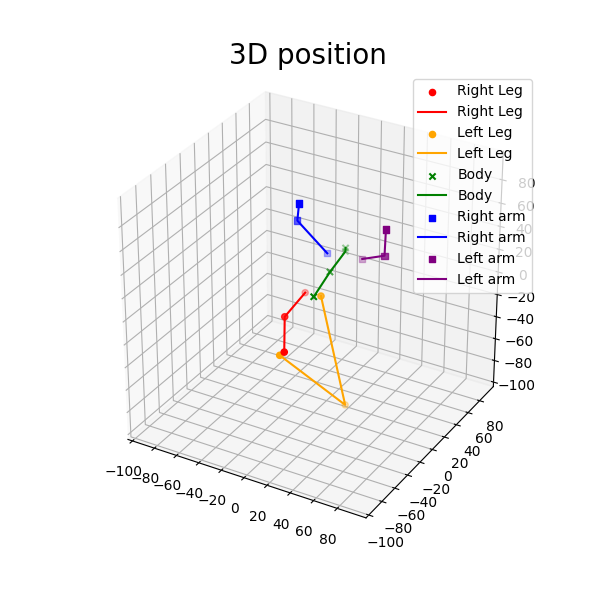
\includegraphics[width=\linewidth]{figure/ch4_fig_bar_result_no1.png}
%       \caption*{(c) 重建結果}
%    \end{minipage}
%    \begin{minipage}{.3\textwidth}
%      \centering
%      \includegraphics[width=\linewidth]{figure/ch4_fig_bar_cam01_no2.jpg}
%      \caption*{(d) cam01 真實影像}
%    \end{minipage}%
%    \begin{minipage}{.3\textwidth}
%       \centering
%       \includegraphics[width=\linewidth]{figure/ch4_fig_bar_cam02_no2.jpg}
%       \caption*{(e) cam02 真實影像}
%     \end{minipage}%
%     \begin{minipage}{.3\textwidth}
%       \centering
%       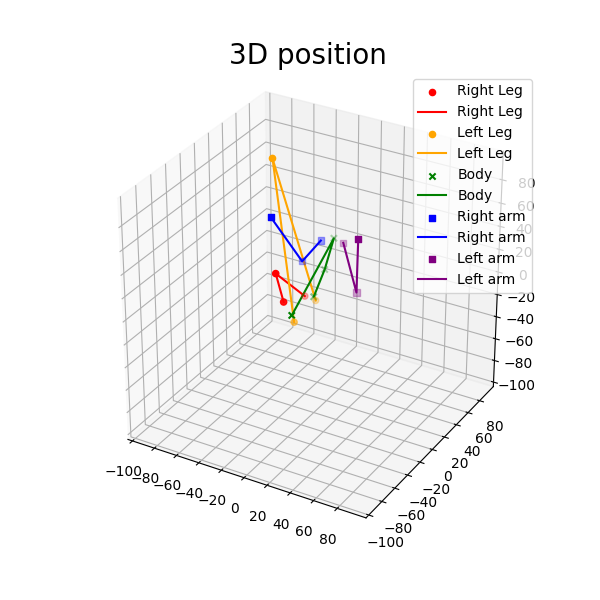
\includegraphics[width=\linewidth]{figure/ch4_fig_bar_result_no2.png}
%       \caption*{(f) 重建結果}
%     \end{minipage}
%    \caption[僅使用影像辨識進行蹲站重建結果]{僅使用影像辨識進行蹲站重建結果}
%    \label{ch4_fig_bar_noimu}
% \end{figure}

% \subsubsection*{蹲站誤差評估}
% 蹲站實驗總計有 1245 幀,每一幀皆估計出人體姿態,每 20 幀進行一次採樣,共計 63 個樣本點進行評估及驗證,可以發現,蹲站實驗中,肢段的平均估計成功率約 11.11\%,平均有效誤差約在 94.5808 (mm)。

% \subsubsection*{開合跳實驗結果}
% \subsubsection*{開合跳誤差評估}
% \subsubsection*{折返跑實驗結果}
% \subsubsection*{折返跑誤差評估}
% \subsubsection*{熱身運動實驗結果}
% \subsubsection*{熱身運動誤差評估}
% \subsubsection*{組合動作實驗結果}
% \subsubsection*{組合動作誤差評估}

% \subsection{結論}
% % 結論
% 123123

% % ------------------------- 4.3 ------------------------- %
% \section{單獨做 IMU 的姿勢估計}
% 單獨 IMU 的結果
% \subsection{實驗設定}
% % 實驗設定
% 123123
% \subsection{實驗執行}
% % 實驗執行
% 123123
% \subsection{誤差評估}
% % 誤差評估
% 123123
% \subsection{結論}
% % 結論
% 123123

% ------------------------- 4.3 ------------------------- %
\section{使用影像辨識融合 IMU 估計姿態}
% sensor fusion 在室內的結果
\subsection{實驗設定}
% 實驗設定
本章節將自行蒐集的資料輸入進學者 Zhe Zhang 等人提出的感測器融合方法中進行人體姿態重建~\cite{Zhang_2020_CVPR}。該方法中包含兩個主要流程,一為影像辨識,二為影像辨識結果融合 IMU 資訊,本章節使用的影像辨識方法為文獻~\cite{Xiao_2018_ECCV} 中,學者 Bin Xiao 等人提出的方法,並套用 Zhe Zhang 等人訓練的 $occlusion\_person\_8view.pth$ 模型進行影像辨識~\cite{zhang2020adafuse},取得記錄關節點於影像中位置的初步熱圖,接著選擇是否融合 IMU 資訊,最後使用三角測量方法計算關節點的三維位置,進而重建人體姿態。

% \subsection{實驗執行}
% % 實驗執行

\subsection{實驗結果與誤差評估}
\subsubsection*{T-pose 實驗結果}
% 用pose_59、172
T-pose 重建結果如圖~\ref{ch4_fig_Tpose} 所示,(a)、(b) 為同一時刻點 cam01 的真實影像及 cam02 的真實影像,(c) 為使用影像辨識融合 IMU 資訊的人體重建結果,(d) 為僅使用影像辨識的人體重建結果。
% ;(e)、(f) 為同一時刻點的 cam01 的真實影像及 cam02 的真實影像,(g) 為使用影像辨識融合 IMU 資訊的人體重建結果,(h) 為僅使用影像辨識的人體重建結果。

\begin{figure}[!ht]
   \centering
   % \begin{minipage}{.25\textwidth}
   %   \centering
   %   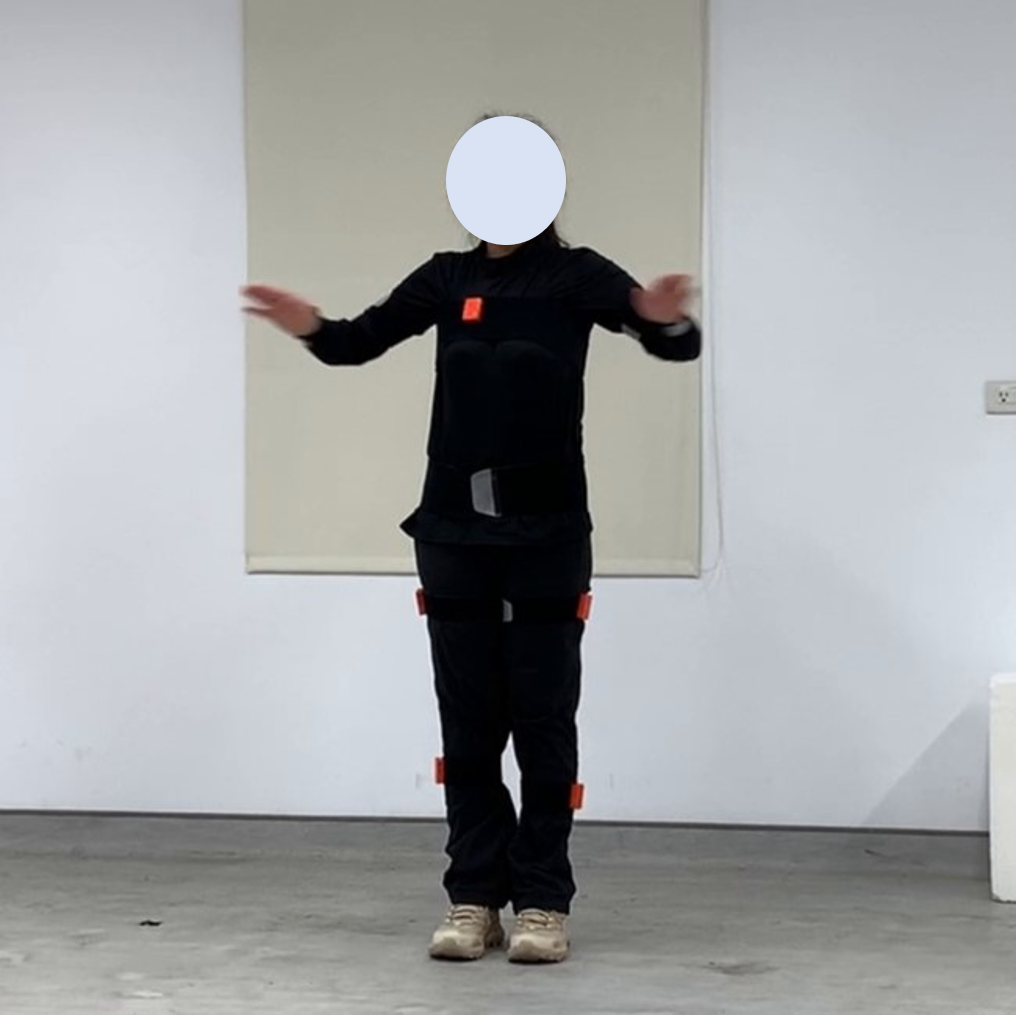
\includegraphics[width=\linewidth]{figure/ch4_fig_tpose_cam01_with1.jpg}
   %   \caption*{(a) cam01 真實影像}
   % \end{minipage}%
   % \begin{minipage}{.25\textwidth}
   %    \centering  
   %    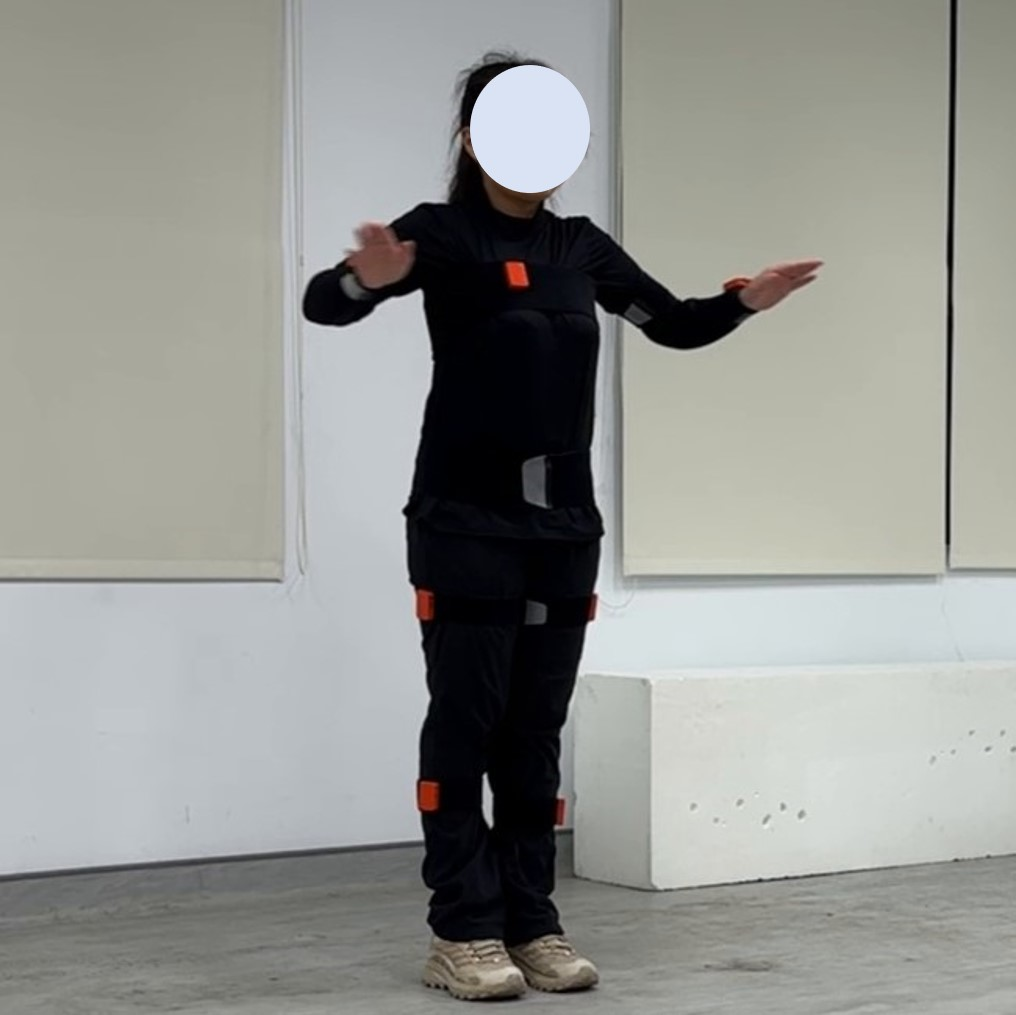
\includegraphics[width=\linewidth]{figure/ch4_fig_tpose_cam02_with1.jpg}
   %    \caption*{(b) cam02 真實影像}
   % \end{minipage}%
   % \begin{minipage}{.25\textwidth}
   %    \centering
   %    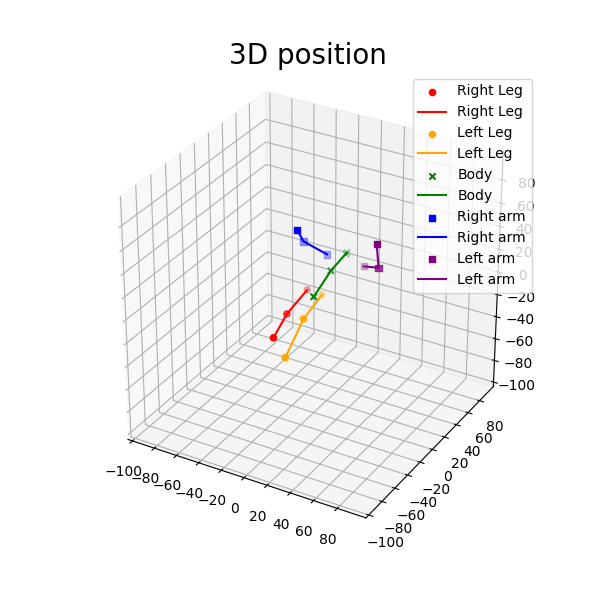
\includegraphics[width=\linewidth]{figure/ch4_fig_tpose_result_with1.png}
   %    \caption*{(c) 影像辨識融合 IMU 重建結果}
   % \end{minipage}%
   % \begin{minipage}{.25\textwidth}
   %    \centering
   %    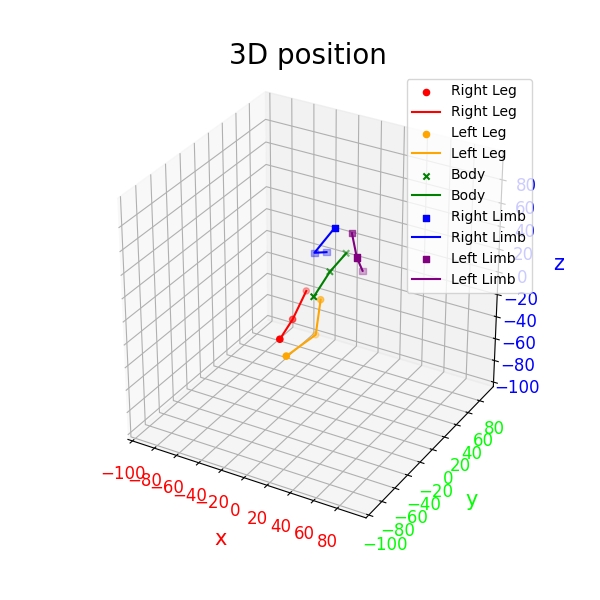
\includegraphics[width=\linewidth]{figure/ch4_fig_tpose_result_no1.png}
   %    \caption*{(d) 影像辨識重建結果}
   % \end{minipage}
   \begin{minipage}{.5\textwidth}
     \centering
     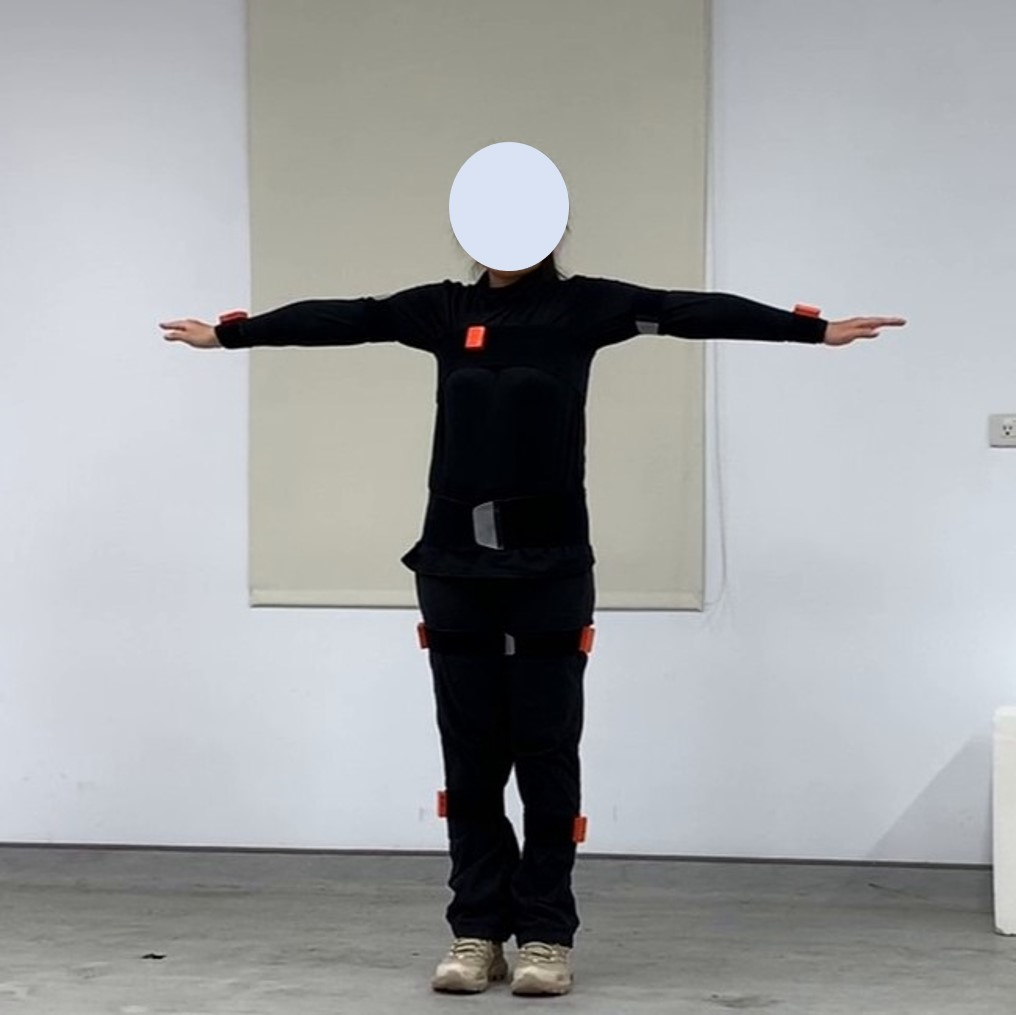
\includegraphics[width=.95\linewidth]{figure/ch4_fig_tpose_cam01_with2.jpg}
     \caption*{(a) cam01 真實影像}
   \end{minipage}%
   \begin{minipage}{.5\textwidth}
      \centering
      \includegraphics[width=.95\linewidth]{figure/ch4_fig_tpose_cam02_with2.jpg}
      \caption*{(b) cam02 真實影像}
   \end{minipage}
   \begin{minipage}{.5\textwidth}
      \centering
      \includegraphics[width=.95\linewidth]{figure/ch4_fig_tpose_result_with2.png}
      \caption*{(c) 影像辨識融合 IMU 重建結果}
   \end{minipage}%
   \begin{minipage}{.5\textwidth}
      \centering
      \includegraphics[width=.95\linewidth]{figure/ch4_fig_tpose_result_no2.png}
      \caption*{(d) 影像辨識重建結果}
   \end{minipage}
   \caption[T-pose 重建結果]{T-pose 重建結果}
   \label{ch4_fig_Tpose}
\end{figure}

\subsubsection*{T-pose 誤差評估}
T-pose 實驗總計有 318 幀,每一幀皆估計出人體姿態,每 20 幀進行一次採樣,共計 16 個樣本點進行評估及驗證,
% 結果如表~\ref{ch4_Tpose_result_withimu} 所示,
可以發現,T-pose 實驗中,影像辨識融合 IMU 資訊的肢段的平均估計成功率約 62.5\%,平均有效誤差約在 82.7502 (mm)。僅使用影像辨識的肢段的平均估計成功率約 12.5\%,平均有效誤差約在 95.0632 (mm)。比較圖~\ref{ch4_fig_Tpose} (c)、(d) 可以發現,僅使用影像辨識建立出來的結果關節點位置會亂飄,影像辨識融合 IMU 朝向資訊的人體重建結果較為接近真實人體姿態。

% \begin{table}[!ht]
%    \caption[影像辨識與 IMU 融合 T-pose 實驗結果與誤差評估]{影像辨識與 IMU 融合 T-pose 實驗結果與誤差評估}
%    \centering
%    \label{ch4_Tpose_result_withimu}
%    \setlength{\tabcolsep}{3pt}
%    \renewcommand\arraystretch{1.5}
%    \resizebox{\textwidth}{!}{
%    \begin{tabular}{c|c|c|c|c|c|c|c|c|c}
%       & {右大腿} & {右小腿} & {左大腿} & {左小腿} & {右上臂} & {右前臂} & {左上臂} & {左前臂} & {平均} \\
%       \midrule[1.5pt]
%       成功幀數 & 317 & 91 & 257 & 245 & 176 & 245 & 41 & 137 & \\
%       成功率 & 99.7 & 28.61 & 80.82 & 77.04 & 55.35 & 77.04 & 12.89 & 43.08 & 59.31 \\
%       \midrule
%       平均估計長度 & \num{322.2769} & \num{277.9209} & \num{328.7976} & \num{295.7648} & \num{273.7784} & \num{227.1334} & \num{238.0457} & \num{277.4777} & \\
%       估計誤差 & \num{52.2303} & \num{82.0791} & \num{36.2124} & \num{69.2352} & \num{33.2216} & \num{12.1334} & \num{56.9543} & \num{66.4777} & \num{51.0680} \\
%    \end{tabular}}
% \end{table}

\clearpage

\subsubsection*{蹲站實驗結果}
% 用pose_225、488
蹲站重建中,站立的實驗結果如圖~\ref{ch4_fig_bar_stand} 所示,(a)、(b) 為同一時刻點 cam01 的真實影像及 cam02 的真實影像,(c) 為使用影像辨識融合 IMU 資訊的人體重建結果,(d) 為僅使用影像辨識的人體重建結果。

\begin{figure}[!ht]
   \centering
   \begin{minipage}{.5\textwidth}
      \centering
      \includegraphics[width=.95\linewidth]{figure/ch4_fig_bar_cam01_with1.jpg}
      \caption*{(a) cam01 真實影像}
    \end{minipage}%
    \begin{minipage}{.5\textwidth}
       \centering
       \includegraphics[width=.95\linewidth]{figure/ch4_fig_bar_cam02_with1.jpg}
       \caption*{(b) cam02 真實影像}
    \end{minipage}
    \begin{minipage}{.5\textwidth}
       \centering
       \includegraphics[width=.95\linewidth]{figure/ch4_fig_bar_result_with1.png}
       \caption*{(c) 影像辨識融合 IMU 重建結果}
    \end{minipage}%
    \begin{minipage}{.5\textwidth}
       \centering
       \includegraphics[width=.95\linewidth]{figure/ch4_fig_bar_result_no1.png}
       \caption*{(d) 影像辨識重建結果}
    \end{minipage}
   \caption[蹲站中站立的重建結果]{蹲站中站立的重建結果}
   \label{ch4_fig_bar_stand}
\end{figure}

\clearpage

蹲下的實驗結果如圖~\ref{ch4_fig_bar_squat} 所示,(a)、(b) 為同一時刻點 cam01 的真實影像及 cam02 的真實影像,(c) 為使用影像辨識融合 IMU 資訊的人體重建結果,(d) 為僅使用影像辨識的人體重建結果。

\begin{figure}[!ht]
   \centering
   \begin{minipage}{.5\textwidth}
      \centering
      \includegraphics[width=.95\linewidth]{figure/ch4_fig_bar_cam01_with2.jpg}
      \caption*{(a) cam01 真實影像}
    \end{minipage}%
    \begin{minipage}{.5\textwidth}
       \centering
       \includegraphics[width=.95\linewidth]{figure/ch4_fig_bar_cam02_with2.jpg}
       \caption*{(b) cam02 真實影像}
    \end{minipage}
    \begin{minipage}{.5\textwidth}
       \centering
       \includegraphics[width=.95\linewidth]{figure/ch4_fig_bar_result_with2.png}
       \caption*{(c) 影像辨識融合 IMU 重建結果}
    \end{minipage}%
    \begin{minipage}{.5\textwidth}
       \centering
       \includegraphics[width=.95\linewidth]{figure/ch4_fig_bar_result_no2.png}
       \caption*{(d) 影像辨識重建結果}
    \end{minipage}
   \caption[蹲站中蹲下的重建結果]{蹲站中蹲下的重建結果}
   \label{ch4_fig_bar_squat}
\end{figure}

\subsubsection*{蹲站誤差評估}
蹲站實驗總計有 1245 幀,每一幀皆估計出人體姿態,每 20 幀進行一次採樣,共計 63 個樣本點進行評估及驗證,可以發現,蹲站實驗中,影像辨識融合 IMU 資訊的肢段的平均估計成功率約 38.1\%,平均有效誤差約在 76.8410 (mm),僅使用影像辨識的肢段的平均估計成功率約 11.11\%,平均有效誤差約在 94.5808 (mm)。從圖~\ref{ch4_fig_bar_stand}、圖~\ref{ch4_fig_bar_squat} (c)、(d) 可以發現,僅使用影像辨識建立的四肢關節點容易亂飄,影像辨識融合 IMU 朝向資訊的人體重建結果,由於加上朝向的限制,所以較為接近真實人體姿態。

\clearpage

\subsubsection*{開合跳實驗結果}
% pose_111、385,候選156.452.449
開合跳實驗重建中,跳起時的實驗結果如圖~\ref{ch4_fig_jump_jump} 所示,(a)、(b) 為同一時刻點 cam01 的真實影像及 cam02 的真實影像,(c) 為使用影像辨識融合 IMU 資訊的人體重建結果,(d) 為僅使用影像辨識的人體重建結果。

\begin{figure}[!ht]
   \centering
   \begin{minipage}{.5\textwidth}
      \centering
      \includegraphics[width=.95\linewidth]{figure/ch4_fig_jump_cam01_with1.jpg}
      \caption*{(a) cam01 真實影像}
    \end{minipage}%
    \begin{minipage}{.5\textwidth}
       \centering
       \includegraphics[width=.95\linewidth]{figure/ch4_fig_jump_cam02_with1.jpg}
       \caption*{(b) cam02 真實影像}
    \end{minipage}
    \begin{minipage}{.5\textwidth}
       \centering
       \includegraphics[width=.95\linewidth]{figure/ch4_fig_jump_result_with1.png}
       \caption*{(c) 影像辨識融合 IMU 重建結果}
    \end{minipage}%
    \begin{minipage}{.5\textwidth}
       \centering
       \includegraphics[width=.95\linewidth]{figure/ch4_fig_jump_result_no1.png}
       \caption*{(d) 影像辨識重建結果}
    \end{minipage}
   \caption[開合跳中跳起時的重建結果]{開合跳中跳起時的重建結果}
   \label{ch4_fig_jump_jump}
\end{figure}

\clearpage

落地時的實驗結果如圖~\ref{ch4_fig_jump_stand} 所示,(a)、(b) 為同一時刻點 cam01 的真實影像及 cam02 的真實影像,(c) 為使用影像辨識融合 IMU 資訊的人體重建結果,(d) 為僅使用影像辨識的人體重建結果。

\begin{figure}[!ht]
   \centering
   \begin{minipage}{.5\textwidth}
      \centering
      \includegraphics[width=.95\linewidth]{figure/ch4_fig_jump_cam01_with2.jpg}
      \caption*{(a) cam01 真實影像}
    \end{minipage}%
    \begin{minipage}{.5\textwidth}
       \centering
       \includegraphics[width=.95\linewidth]{figure/ch4_fig_jump_cam02_with2.jpg}
       \caption*{(b) cam02 真實影像}
    \end{minipage}
    \begin{minipage}{.5\textwidth}
       \centering
       \includegraphics[width=.95\linewidth]{figure/ch4_fig_jump_result_with2.png}
       \caption*{(c) 影像辨識融合 IMU 重建結果}
    \end{minipage}%
    \begin{minipage}{.5\textwidth}
       \centering
       \includegraphics[width=.95\linewidth]{figure/ch4_fig_jump_result_no2.png}
       \caption*{(d) 影像辨識重建結果}
    \end{minipage}
   \caption[開合跳中落地時的重建結果]{開合跳中落地時的重建結果}
   \label{ch4_fig_jump_stand}
\end{figure}

\subsubsection*{開合跳誤差評估}
開合跳實驗總計有 664 幀,每一幀皆估計出人體姿態,每 20 幀進行一次採樣,共計 34 個樣本點進行評估及驗證,可以發現,開合跳實驗中,影像辨識融合 IMU 資訊的肢段的平均估計成功率約 50\%,平均有效誤差約在 80.8609 (mm),僅使用影像辨識的肢段的平均估計成功率約 35.29\%,平均有效誤差約在 76.4560 (mm)。從圖~\ref{ch4_fig_jump_jump}、圖~\ref{ch4_fig_jump_stand} (c)、(d) 可以發現,僅使用影像辨識建立的四肢關節點容易亂飄,影像辨識融合 IMU 朝向資訊的人體重建結果,由於加上朝向的限制,所以較為接近真實人體姿態,且儘管因為動作變化快速,造成影像動態模糊問題,融合 IMU 資訊後仍可以成功重建四肢的姿態,但是,在圖中可以看到有綠色的點飄到邊界外,該點為鼻子關鍵點,由於在開合跳落地時,受試者的臉皆為模糊的狀態,因此影像辨識無法辨識出鼻子,且頭部沒有黏貼任何 IMU,因此鼻子的位置在這個情境下較難重建成功。
% 而在圖~\ref{ch4_fig_jump_stand} (c)、(d) 中,頭部可以發現頭部的位置點明顯超出邊界。

\clearpage

\subsubsection*{折返跑實驗結果}
% pose_123、314、1045,在300、422可以看到影像辨識把左右邊搞混的現象
折返跑實驗重建中,跑步時的實驗結果如圖~\ref{ch4_fig_run_run} 所示,(a)、(b) 為同一時刻點 cam01 的真實影像及 cam02 的真實影像,(c) 為使用影像辨識融合 IMU 資訊的人體重建結果,(d) 為僅使用影像辨識的人體重建結果。

\begin{figure}[!ht]
   \centering
   \begin{minipage}{.5\textwidth}
      \centering
      \includegraphics[width=.95\linewidth]{figure/ch4_fig_run_cam01_with1.jpg}
      \caption*{(a) cam01 真實影像}
    \end{minipage}%
    \begin{minipage}{.5\textwidth}
       \centering
       \includegraphics[width=.95\linewidth]{figure/ch4_fig_run_cam02_with1.jpg}
       \caption*{(b) cam02 真實影像}
    \end{minipage}
    \begin{minipage}{.5\textwidth}
       \centering
       \includegraphics[width=.95\linewidth]{figure/ch4_fig_run_result_with1.png}
       \caption*{(c) 影像辨識融合 IMU 重建結果}
    \end{minipage}%
    \begin{minipage}{.5\textwidth}
       \centering
       \includegraphics[width=.95\linewidth]{figure/ch4_fig_run_result_no1.png}
       \caption*{(d) 影像辨識重建結果}
    \end{minipage}
   \caption[折返跑中跑步時的重建結果]{折返跑中跑步時的重建結果}
   \label{ch4_fig_run_run}
\end{figure}

\clearpage

轉身時的實驗結果如圖~\ref{ch4_fig_run_turn} 所示,(a)、(b) 為同一時刻點 cam01 的真實影像及 cam02 的真實影像,(c) 為使用影像辨識融合 IMU 資訊的人體重建結果,(d) 為僅使用影像辨識的人體重建結果。

\begin{figure}[!ht]
   \centering
   \begin{minipage}{.5\textwidth}
      \centering
      \includegraphics[width=.95\linewidth]{figure/ch4_fig_run_cam01_with2.jpg}
      \caption*{(a) cam01 真實影像}
    \end{minipage}%
    \begin{minipage}{.5\textwidth}
       \centering
       \includegraphics[width=.95\linewidth]{figure/ch4_fig_run_cam02_with2.jpg}
       \caption*{(b) cam02 真實影像}
    \end{minipage}
    \begin{minipage}{.5\textwidth}
       \centering
       \includegraphics[width=.95\linewidth]{figure/ch4_fig_run_result_with2.png}
       \caption*{(c) 影像辨識融合 IMU 重建結果}
    \end{minipage}%
    \begin{minipage}{.5\textwidth}
       \centering
       \includegraphics[width=.95\linewidth]{figure/ch4_fig_run_result_no2.png}
       \caption*{(d) 影像辨識重建結果}
    \end{minipage}
   \caption[折返跑中轉身時的重建結果]{折返跑中轉身時的重建結果}
   \label{ch4_fig_run_turn}
\end{figure}

\clearpage

手摸地時的實驗結果如圖~\ref{ch4_fig_run_touch} 所示,(a)、(b) 為同一時刻點 cam01 的真實影像及 cam02 的真實影像,(c) 為使用影像辨識融合 IMU 資訊的人體重建結果,(d) 為僅使用影像辨識的人體重建結果。

\begin{figure}[!ht]
   \centering
   \begin{minipage}{.5\textwidth}
      \centering
      \includegraphics[width=.95\linewidth]{figure/ch4_fig_run_cam01_with3.jpg}
      \caption*{(a) cam01 真實影像}
    \end{minipage}%
    \begin{minipage}{.5\textwidth}
       \centering
       \includegraphics[width=.95\linewidth]{figure/ch4_fig_run_cam02_with3.jpg}
       \caption*{(b) cam02 真實影像}
    \end{minipage}
    \begin{minipage}{.5\textwidth}
       \centering
       \includegraphics[width=.95\linewidth]{figure/ch4_fig_run_result_with3.png}
       \caption*{(c) 影像辨識融合 IMU 重建結果}
    \end{minipage}%
    \begin{minipage}{.5\textwidth}
       \centering
       \includegraphics[width=.95\linewidth]{figure/ch4_fig_run_result_no3.png}
       \caption*{(d) 影像辨識重建結果}
    \end{minipage}
   \caption[折返跑中手摸地時的重建結果]{折返跑中手摸地時的重建結果}
   \label{ch4_fig_run_touch}
\end{figure}

\subsubsection*{折返跑誤差評估}
折返跑實驗總計有 1609 幀,每一幀皆估計出人體姿態,每 20 幀進行一次採樣,共計 81 個樣本點進行評估及驗證,可以發現,折返跑實驗中,影像辨識融合 IMU 資訊的肢段的平均估計成功率約 53.09\%,平均有效誤差約在 82.6446 (mm),僅使用影像辨識的肢段的平均估計成功率約 40.74\%,平均有效誤差約在 80.0463 (mm)。從圖~\ref{ch4_fig_run_run}、圖~\ref{ch4_fig_run_turn}、圖~\ref{ch4_fig_run_touch} (c)、(d) 可以發現,影像辨識融合 IMU 朝向資訊的人體重建結果,由於加上朝向的限制,所以較為接近真實人體姿態,且即使是圖~\ref{ch4_fig_run_run} 中,有一半關節被遮擋的情境下也可以成功建立。

\clearpage

\subsubsection*{熱身運動實驗結果}
% pose_594、818、1622、1786,上半身伸展備用410、510、596,肩膀伸展比較屬於正面運動119、151、229、287,腿部拉筋備用778、889,蹲下姿勢1277、1280
熱身運動實驗重建中,腰部伸展時的實驗結果如圖~\ref{ch4_fig_warm_warm} 所示,(a)、(b) 為同一時刻點 cam01 的真實影像及 cam02 的真實影像,(c) 為使用影像辨識融合 IMU 資訊的人體重建結果,(d) 為僅使用影像辨識的人體重建結果。

\begin{figure}[!ht]
   \centering
   \begin{minipage}{.5\textwidth}
      \centering
      \includegraphics[width=.95\linewidth]{figure/ch4_fig_warm_cam01_with1.jpg}
      \caption*{(a) cam01 真實影像}
    \end{minipage}%
    \begin{minipage}{.5\textwidth}
       \centering
       \includegraphics[width=.95\linewidth]{figure/ch4_fig_warm_cam02_with1.jpg}
       \caption*{(b) cam02 真實影像}
    \end{minipage}
    \begin{minipage}{.5\textwidth}
       \centering
       \includegraphics[width=.95\linewidth]{figure/ch4_fig_warm_result_with1.png}
       \caption*{(c) 影像辨識融合 IMU 重建結果}
    \end{minipage}%
    \begin{minipage}{.5\textwidth}
       \centering
       \includegraphics[width=.95\linewidth]{figure/ch4_fig_warm_result_no1.png}
       \caption*{(d) 影像辨識重建結果}
    \end{minipage}
   \caption[熱身運動中腰部伸展時的重建結果]{熱身運動中腰部伸展時的重建結果}
   \label{ch4_fig_warm_warm}
\end{figure}

\clearpage

側面腿部伸展側身時的實驗結果如圖~\ref{ch4_fig_warm_side} 所示,(a)、(b) 為同一時刻點 cam01 的真實影像及 cam02 的真實影像,(c) 為使用影像辨識融合 IMU 資訊的人體重建結果,(d) 為僅使用影像辨識的人體重建結果。

\begin{figure}[!ht]
   \centering
   \begin{minipage}{.5\textwidth}
      \centering
      \includegraphics[width=.95\linewidth]{figure/ch4_fig_warm_cam01_with2.jpg}
      \caption*{(a) cam01 真實影像}
    \end{minipage}%
    \begin{minipage}{.5\textwidth}
       \centering
       \includegraphics[width=.95\linewidth]{figure/ch4_fig_warm_cam02_with2.jpg}
       \caption*{(b) cam02 真實影像}
    \end{minipage}
    \begin{minipage}{.5\textwidth}
       \centering
       \includegraphics[width=.95\linewidth]{figure/ch4_fig_warm_result_with2.png}
       \caption*{(c) 影像辨識融合 IMU 重建結果}
    \end{minipage}%
    \begin{minipage}{.5\textwidth}
       \centering
       \includegraphics[width=.95\linewidth]{figure/ch4_fig_warm_result_no2.png}
       \caption*{(d) 影像辨識重建結果}
    \end{minipage}
   \caption[熱身運動中側面腿部伸展側身時的重建結果]{熱身運動中側面腿部伸展側身時的重建結果}
   \label{ch4_fig_warm_side}
\end{figure}

\clearpage

正面腿部伸展時的實驗結果如圖~\ref{ch4_fig_warm_front} 所示,(a)、(b) 為同一時刻點 cam01 的真實影像及 cam02 的真實影像,(c) 為使用影像辨識融合 IMU 資訊的人體重建結果,(d) 為僅使用影像辨識的人體重建結果。

\begin{figure}[!ht]
   \centering
   \begin{minipage}{.5\textwidth}
      \centering
      \includegraphics[width=.95\linewidth]{figure/ch4_fig_warm_cam01_with3.jpg}
      \caption*{(a) cam01 真實影像}
    \end{minipage}%
    \begin{minipage}{.5\textwidth}
       \centering
       \includegraphics[width=.95\linewidth]{figure/ch4_fig_warm_cam02_with3.jpg}
       \caption*{(b) cam02 真實影像}
    \end{minipage}
    \begin{minipage}{.5\textwidth}
       \centering
       \includegraphics[width=.95\linewidth]{figure/ch4_fig_warm_result_with3.png}
       \caption*{(c) 影像辨識融合 IMU 重建結果}
    \end{minipage}%
    \begin{minipage}{.5\textwidth}
       \centering
       \includegraphics[width=.95\linewidth]{figure/ch4_fig_warm_result_no3.png}
       \caption*{(d) 影像辨識重建結果}
    \end{minipage}
   \caption[熱身運動中正面腿部伸展時的重建結果]{熱身運動中跑步時的重建結果}
   \label{ch4_fig_warm_front}
\end{figure}

\clearpage

背面腿部伸展時的實驗結果如圖~\ref{ch4_fig_warm_back} 所示,(a)、(b) 為同一時刻點 cam01 的真實影像及 cam02 的真實影像,(c) 為使用影像辨識融合 IMU 資訊的人體重建結果,(d) 為僅使用影像辨識的人體重建結果。

\begin{figure}[!ht]
   \centering
   \begin{minipage}{.5\textwidth}
      \centering
      \includegraphics[width=.95\linewidth]{figure/ch4_fig_warm_cam01_with4.jpg}
      \caption*{(a) cam01 真實影像}
    \end{minipage}%
    \begin{minipage}{.5\textwidth}
       \centering
       \includegraphics[width=.95\linewidth]{figure/ch4_fig_warm_cam02_with4.jpg}
       \caption*{(b) cam02 真實影像}
    \end{minipage}
    \begin{minipage}{.5\textwidth}
       \centering
       \includegraphics[width=.95\linewidth]{figure/ch4_fig_warm_result_with4.png}
       \caption*{(c) 影像辨識融合 IMU 重建結果}
    \end{minipage}%
    \begin{minipage}{.5\textwidth}
       \centering
       \includegraphics[width=.95\linewidth]{figure/ch4_fig_warm_result_no4.png}
       \caption*{(d) 影像辨識重建結果}
    \end{minipage}
   \caption[熱身運動中背面腿部伸展時的重建結果]{熱身運動中背面腿部伸展時的重建結果}
   \label{ch4_fig_warm_back}
\end{figure}

\subsubsection*{熱身運動誤差評估}
熱身運動實驗總計有 2135 幀,每一幀皆估計出人體姿態,每 20 幀進行一次採樣,共計 107 個樣本點進行評估及驗證,可以發現,熱身運動實驗中,影像辨識融合 IMU 資訊的肢段的平均估計成功率約 46.73\%,平均有效誤差約在 7.5974 (mm),僅使用影像辨識的肢段的平均估計成功率約 31.78\%,平均有效誤差約在 67.2949 (mm)。從圖~\ref{ch4_fig_warm_warm}、圖~\ref{ch4_fig_warm_side}、圖~\ref{ch4_fig_warm_front}、圖~\ref{ch4_fig_warm_back} (c)、(d) 可以發現,影像辨識融合 IMU 朝向資訊的人體重建結果,由於加上朝向的限制,所以較為接近真實人體姿態,且即使是圖~\ref{ch4_fig_warm_side} 中,有一半關節被遮擋的情境下也可以成功建立,但在圖~\ref{ch4_fig_warm_back} 中,可以發現重建的效果較差,可能是因為影像辨識模型並沒有被訓練辨識背面的影像,因此影像辨識較難成功。

% \subsubsection*{組合動作實驗結果}
% \subsubsection*{組合動作誤差評估}
\subsection{結論}
% 結論
將以上實驗的成功率與誤差整理成表格,如表~\ref{ch4_tab_conclusion} 所示。
\begin{table}[ht!]
   \caption{影像辨識有無融合 IMU 的結果比較}
   \label{ch4_tab_conclusion}
   \centering
   \begin{tabular}{ccccccc}
   \toprule
    & IMU 融合 & T-pose & 蹲站 & 開合跳 & 折返跑 & 熱身運動 \\
   \midrule
   \multirow{2}{*}{誤差 (mm)} & O & 82.7502 & 76.8410 & 80.8609 & 82.6446 & 75.9740 \\
   & X & 95.0632 & 94.5808 & 76.4561 & 80.0463 & 67.2949 \\
   \midrule
   \multirow{2}{*}{成功率 (\%)} & O & 62.50 & 38.10 & 50.00 & 53.09 & 46.73 \\
   & X & 12.50 & 11.11 & 35.29 & 40.74 & 31.78 \\
   \bottomrule
   \end{tabular}
\end{table}

可以發現,影像辨識融合 IMU 資訊的肢段的平均估計成功率皆高於僅使用影像辨識的肢段,如圖~\ref{ch4_fig_error_success} (a) 所示,平均約有 23.8\% 的提升,本研究推斷,在 T-pose 有顯著提升的原因為在實驗過程中受試者皆靜止不動,相較其他實驗過程中,受試者有執行指定動作,因此 IMU 朝向資訊在 T-pose 實驗過程中,除量測誤差外的其餘誤差較小,因此加上 IMU 的朝向資訊後,成功率有顯著提升。而影像辨識融合 IMU 資訊的肢段的平均有效誤差則如圖~\ref{ch4_fig_error_success} (b) 所示,在 T-pose 實驗與蹲站實驗的誤差比較中,影像辨識融合 IMU 資訊重建人體姿態相較僅使用影像辨識重建人體姿態有約 10 (mm) 的改善,而在開合跳、折返跑、熱身運動中,影像辨識融合 IMU 資訊重建人體姿態相較僅使用影像辨識重建人體姿態誤差約提升 5 \textasciitilde\ 10 (mm),本研究推斷,造成此現象的原因可能是這三組動作較為複雜,造成影像辨識關節點較為困難,使得辨識結果較差,而 IMU 朝向資訊雖然可以提供方向資訊,但是在這三組動作中,受試者的動作較快速,且量測時間較長,因此在 IMU 整合朝向資訊時產生誤差。整體而言,將影像辨識結果融合 IMU 後,無論是誤差有所改善或是沒有明顯增加,在重建成功率上都有所提升,因此本研究推斷,影像辨識融合 IMU 資訊的方法可以提升影像辨識的成功率,且改善影像辨識的重建結果。

\begin{figure}[!ht]
   \centering
   \begin{minipage}{\textwidth}
     \centering
     \includegraphics[width=\linewidth]{figure/ch4_fig_error.png}
     \caption*{(a) 誤差}
   \end{minipage}
   \begin{minipage}{\textwidth}
      \centering
      \includegraphics[width=\linewidth]{figure/ch4_fig_success.png}
      \caption*{(b) 重建成功率}
   \end{minipage}
   \caption[是否融合 IMU 的誤差及成功率比較]{是否融合 IMU 的誤差及成功率比較}
   \label{ch4_fig_error_success}
\end{figure}

\clearpage

% % ------------------------- 4.5 ------------------------- %
% \section{使用影像辨識融合 IMU 於室外估計姿態}
% sensor fusion 在室外的結果
% \subsection{實驗設定}
% % 實驗設定
% 123123
% % \subsection{實驗執行}
% % % 實驗執行
% % 123123
% \subsection{誤差評估}
% % 誤差評估
% 123123
% \subsection{結論}
% % 結論
% 123123

% ------------------------- 4.5 ------------------------- %
\section{小結}
% 回顧;下章節再討論;從驗證結果證實方法有效
本章節首先透過先前學者們提出的資料集與影像辨識融合 IMU 方法,探討減少相機使用數量對於人體姿態估計精準度的影響,若容許誤差 100 (mm),則可以選擇兩台相機或三台相機進行姿勢估計。此外,本研究提出使用影像辨識及三角測量計算方法建立三維人體模型,用於將 IMU 朝向資訊轉換為位置資訊,並透過先前學者們提出的資料集進行驗證,整體平均誤差約為 25.75 (mm)。最後本研究透過 T-pose 、蹲站、開合跳、折返跑、熱身運動等實驗,驗證融合 IMU 資訊是否對於影像辨識重建人體姿態有所改善,結果顯示,影像辨識融合 IMU 的方法可以提升影像辨識的成功率,且改善影像辨識的重建結果,因此本研究推斷,影像辨識融合 IMU 資訊的方法可以提升影像辨識的成功率,且改善影像辨識的重建結果。下一章將統整本研究的結論及貢獻,並提出相關的未來工作。

\clearpage
\chapter{結論與未來工作}
\fontsize{12pt}{18pt}\selectfont

% ------------------------- 6.0 ------------------------- %
在本論文中,首先於第一章介紹人體姿態量測、估計與重建的研究背景,以及每種方法的量測限制,衍生出本論文的動機與目的;接著於第二章介紹相關的研究文獻,並針對相關的文獻及應用進行回顧與探討;再來於第三章本研究所使用的研究方法,透過整系列的研究方法來進行實驗設置及資料前處理,旨在減少設備成本及架設時間,並使每位受試者都可以自行處理蒐集到的資料並進行感測器融合,從而重建人體姿態;第四章驗證減少設備使用數量的可行性、確認建立個人化三維人體模型的準確度,並藉由選擇有無融合 IMU 資訊驗證影像辨識融合 IMU 資訊可以有效提高人體姿態重建的成功率,並且解除對 Vicon 的依賴。最後,本章節將依序列出本研究的成果與貢獻,並提出三項未來工作,作為本研究可延伸之方向。

% ------------------------- 6.1 ------------------------- %
\section{研究成果與貢獻}
下方將條列出數個關於本研究之成果與貢獻,讓讀者除了回顧本論文之核心方法外,也能清楚瞭解該論文之成果與貢獻處。

\begin{itemize}
    \item \textbf{探討減少相機數量對人體姿態重建精準度的影響}
    \\ 本研究基於文獻~\cite{Zhang_2020_CVPR},使用其提出的感測器融合方法及 TotalCapture Dataset ~\cite{Trumble:BMVC:2017} 進行探討,TotalCapture Dataset 提供 8 台相機的影像資料、13 個 IMU 資料及 Vicon 資料的。本研究固定輸入 8 個 IMU 資料,並藉由選擇輸入相機數量及相機配對,探討減少相機數量對人體姿態重建精準度的影響。
    \clearpage
    \item \textbf{應用影像辨識及三角測量計算建立三維人體模型}
    \\ 本研究提出使用影像辨識及三角測量計算方法建立三維人體模型,取代由 Vicon 資訊建立的三維人體模型,並透過該模型將 IMU 朝向資料轉換成三維位置資料,以供後續進行感測器融合,並進行人體姿態重建。
    \item \textbf{建立用於輸入感測器融合程式的資料前處理流程}
    \\ 本研究提出一系列資料前處理流程,包含相機校正、個人化三維人體模型建立、時間同步、空間校正等流程,以供每位受試者皆可自行處理資料,並輸入感測器融合程式進行人體姿態重建。
    \item \textbf{驗證影像辨識融合 IMU 資訊可以有效提高人體姿態重建的成功率}
    \\ 本研究進行蹲站、開合跳、折返跑、熱身運動等實驗,並透過選擇有無融合 IMU 資訊重建人體姿態,來驗證影像辨識融合 IMU 資訊可以有效提高人體姿態重建的成功率,並且在不需 Vicon 資訊的情況下,也可進行人體姿態重建。
\end{itemize}

% ------------------------- 6.2 ------------------------- %
\section{未來工作}
下方將列舉幾個未來工作,可作為本研究之延伸方向:

\begin{itemize}
    \item \textbf{解除對背景、衣著的限制}
    \\ 本研究目前使用的影像辨識模型由於訓練資料庫較單一,對於受試者、服裝、環境的容忍度較低,難以廣泛應用,因此未來可嘗試解除對背景、衣著的限制,使得該方法更具廣泛性。
    \item \textbf{探討相機擺放角度對人體姿態重建的影響}
    \\ 造成影像辨識融合 IMU 資訊估計人體姿態的誤差的原因除了影像辨識模型的精準度及 IMU 資訊的精準度外,相機擺放角度也是一個重要因素,因此未來可探討相機擺放角度對人體姿態重建的影響。
    \item \textbf{量化重建姿態與原始姿態的相似程度}
    \\ 目前本研究僅透過視覺觀察重建姿態與原始姿態的相似程度,未來可透過量化的方法來評估重建姿態與原始姿態的相似程度,以提高評估的客觀性。
\end{itemize}

\clearpage

%---------- Input your reference here ---------
\bibliographystyle{unsrt}
\addcontentsline{toc}{chapter}{\bibname}
\bibliography{thesis}

% %----------- Input your appendix here  -----------
\appendix
\titlecontents{chapter}[0em]{\fontsize{12}{18}\selectfont}
{\hspace{3.5em}\contentslabel[附錄\,\thecontentslabel]{3.5em}}
{}{\hspace{0.5em}\titlerule*{.}\contentspage}

\titleformat{\chapter}[display]
{\bf\Large}
{\filleft 附錄\,\thechapter}
{1ex}
{\huge\titlerule
	\vspace{2ex}%
	\filright}
[\vspace{2ex}%
	\titlerule]

\chapter{六台相機、七台相機實驗結果}\label{appendix:6cam7cam}
\fontsize{12pt}{18pt}\selectfont

% ------------------------- 5.0 ------------------------- %
% 概述;本章安排
\section{使用六台相機及八個 IMU 進行人體姿態重建結果}
\begin{table}[!ht]
    \caption[六台相機組合與其估計結果誤差]{六台相機組合與其估計結果誤差}
    \centering
    %\label{ch3_cameraset_2cam}
    \setlength{\tabcolsep}{3pt}
    \renewcommand\arraystretch{1.5}
    \resizebox{\textwidth}{!}{
    \begin{tabular}{
    >{\columncolor[HTML]{E7E6E6}}c |c|
    >{\columncolor[HTML]{E7E6E6}}c |c|
    >{\columncolor[HTML]{E7E6E6}}c |c|
    >{\columncolor[HTML]{E7E6E6}}c |c}
       相機組合 & MPJPE & 相機組合 & MPJPE & 相機組合 & MPJPE & 相機組合 & MPJPE \\
       \hline
        123456 & 26.8215 & 123457 & 24.9722 & 123458 & 25.5851 & 123467 & 26.6366 \\
        123468 & 26.6403 & 123478 & 25.9450 & 123567 & 25.3907 & 123568 & 26.0888 \\
        123578 & 24.9857 & 123678 & 26.1367 & 124567 & 26.3538 & 124568 & 27.2836 \\
        124578 & 26.2943 & 124678 & 26.6054 & 125678 & 26.9609 &        &         \\
        \hline
        134567 & 24.3427 & 134568 & 24.5231 & 134578 & 23.4599 & 134678 & 24.1122 \\
        135678 & 23.8219 & 145678 & 24.5035 &        &         &        &         \\
        \hline
        234567 & 28.3596 & 234568 & 27.7637 & 234578 & 26.3288 & 234678 & 28.3135 \\
        235678 & 26.9275 & 245678 & 27.6373 & 345678 & 25.1506 &        &         \\
    \end{tabular}}
 \end{table}

\clearpage

\section{使用七台相機及八個 IMU 進行人體姿態重建結果}
\begin{table}[!ht]
    \caption[七台相機組合與其估計結果誤差]{七台相機組合與其估計結果誤差}
    \centering
    %\label{ch3_cameraset_1cam}
    \setlength{\tabcolsep}{3pt}
    \renewcommand\arraystretch{1.5}
    \resizebox{\textwidth}{!}{
    \begin{tabular}{
    >{\columncolor[HTML]{E7E6E6}}c |c|
    >{\columncolor[HTML]{E7E6E6}}c |c|
    >{\columncolor[HTML]{E7E6E6}}c |c|
    >{\columncolor[HTML]{E7E6E6}}c |c}
       相機編號 & MPJPE & 相機編號 & MPJPE & 相機編號 & MPJPE & 相機編號 & MPJPE \\
       \hline
        1234567 & 25.0931 & 1234568 & 25.2446 & 1234578 & 24.2100 & 1234678 & 25.2497 \\
        1235678 & 24.5841 & 1245678 & 25.4337 & 1345678 & 23.3984 & 2345678 & 26.2036 \\
    \end{tabular}}
 \end{table}

\clearpage

\backmatter

\end{document}

%
%                     ooOoo       
%                   o8888888o            
%                   88" . "88            
%                   (| -_- |)          
%                   O\  =  /O            
%                 ___/`---'\___            
%              .'  \\|     |//  `.          
%             /  \\|||  :  |||//  \            
%            /  _||||| -:- |||||-  \         
%            |   | \\\  -  /// |   |           
%            | \_|  ''\---/''  |   |           
%             \  .-\__  -  ___/-. /            
%           ___. .'  /--.--\  . . ___         
%       ."" '<  `.___\_<|>_/___.'  >'"".        
%        | | :  - \.;`\ _ /`;.`/ - ` : | |     
%       \  \ -.   \_ __\ /__ _/   .- /  /           
%   =====`-.____-.___\_____/___.-____.-'=====    
%                    `=---='                        
%  ^^^^^^^^^^^^^^^^^^^^^^^^^^^^^^^^^^^^^^^^^^^^  
%            佛祖庇佑         永無BUG     
%
% (僅代表可悲的人體組傳承宥廷學長的好運佛祖)